\documentclass[aspectratio=169,xcolor=dvipsnames]{beamer}

\usetheme{Warsaw}
%\usepackage{appendixnumberbeamer}
%\usefonttheme{serif}
\usefonttheme[onlymath]{serif} %options:stillsansseriflarge,stillsansserifmath

\usepackage[numbers,sort&compress]{natbib}
\usepackage{booktabs}
\usepackage[scale=2]{ccicons}
\usepackage{relsize}
\usepackage{amsmath}
\usepackage{bm}
\usepackage{xspace}
\usepackage[normalem]{ulem}
\usepackage{braket}
\usepackage[thicklines]{cancel}
\usepackage{varwidth}
\usepackage[export]{adjustbox}
\usepackage{listings}
\usepackage{wasysym}
\usepackage{tabu}
\usepackage{relsize}
\usepackage{caption}
\usepackage{tcolorbox}
\usepackage{siunitx}
\usepackage{lmodern}
\usepackage{float}% If comment this, figure moves to Page 2
\usepackage{tabu}
\usepackage{multirow}
\usepackage{array}
%\newcommand{\themename}{\textbf{\textsc{metropolis}}\xspace}
\pagenumbering{roman}

\title{PID efficiencies}
% \subtitle{Subtítulo}
% \date{\today}
\date{}
\author{Shuo Jia}
%\institute{UFPR - Disciplina - Semestre}
%\setbeamertemplate{footline}[frame number]

\begin{document}
\maketitle

%\begin{frame}{Table of contents}
%  \setbeamertemplate{section in toc}[sections numbered]
%  \tableofcontents[hideallsubsections]
%\end{frame}
%\section{Introduction}



\begin{frame}{HMS,electron arm}
    %\begin{tabular}{S} \toprule
  \begin{block}{Basic cuts}
    cointime:2.5(fall)/1.5(spring) \\
    HMS(SHMS) delta:-8,8(-10,20)  \\
    HMS(SHMS) acceptance constrain \\
    SHMS pi cut \\
    accidental background: 6 peaks \\
  \end{block}
  \begin{columns}
    \begin{column}[T]{0.5\textwidth}
     \begin{block}{HMS Calorimeter}
       Cherenkov cut: 12 \\
       Calorimeter cut: varies
     \end{block}
   \end{column}
   \begin{column}[T]{0.5\textwidth}
     \begin{block}{HMS Cherenkov}
       Cherenkov cut: varies \\
       Calorimeter cut: 1
       \end{block}
     \end{column}
   \end{columns}
    %\end{tabular}
    %\begin{tabular}{|c|c|c|}
    %  \hline
    %  Cuts & HMS cal & HMS cer\\ 
    %  \hline
    %  cointime & 1.5/2.5 & same\\
    %  \hline
    %  H dp & -8,8 & same\\
    %  \hline
    %  P dp & -10,20 & same\\
    %  \hline
    %  H xptar & -0.06,0.06 & same\\
    %  \hline
    %  H yptar & -0.022,0.022 & same\\
    %  \hline
    %  P xptar & -0.045,0.045 & same\\
    %  \hline
    %  P yptar & -0.028,0.028 & same\\
    %  \hline
    %  bg & -3,+3 & same\\
    %  \hline
    %  P cal & 0.05,0.85 & same\\
    %  \hline
    %  P hgcer & no & no \\
    %  \hline
    %  P rf & 0.5,1.5 & same\\
    %  \hline
    %  P aero & 2 & same\\
    %  \hline
    %  H cal & varies & 1\\
    %  \hline 
    %  H cer & 10 &varies \\
    %  \hline
    %\end{tabular}
\end{frame}{}
\begin{frame}{HMS Cer, not a good pion rejector}
  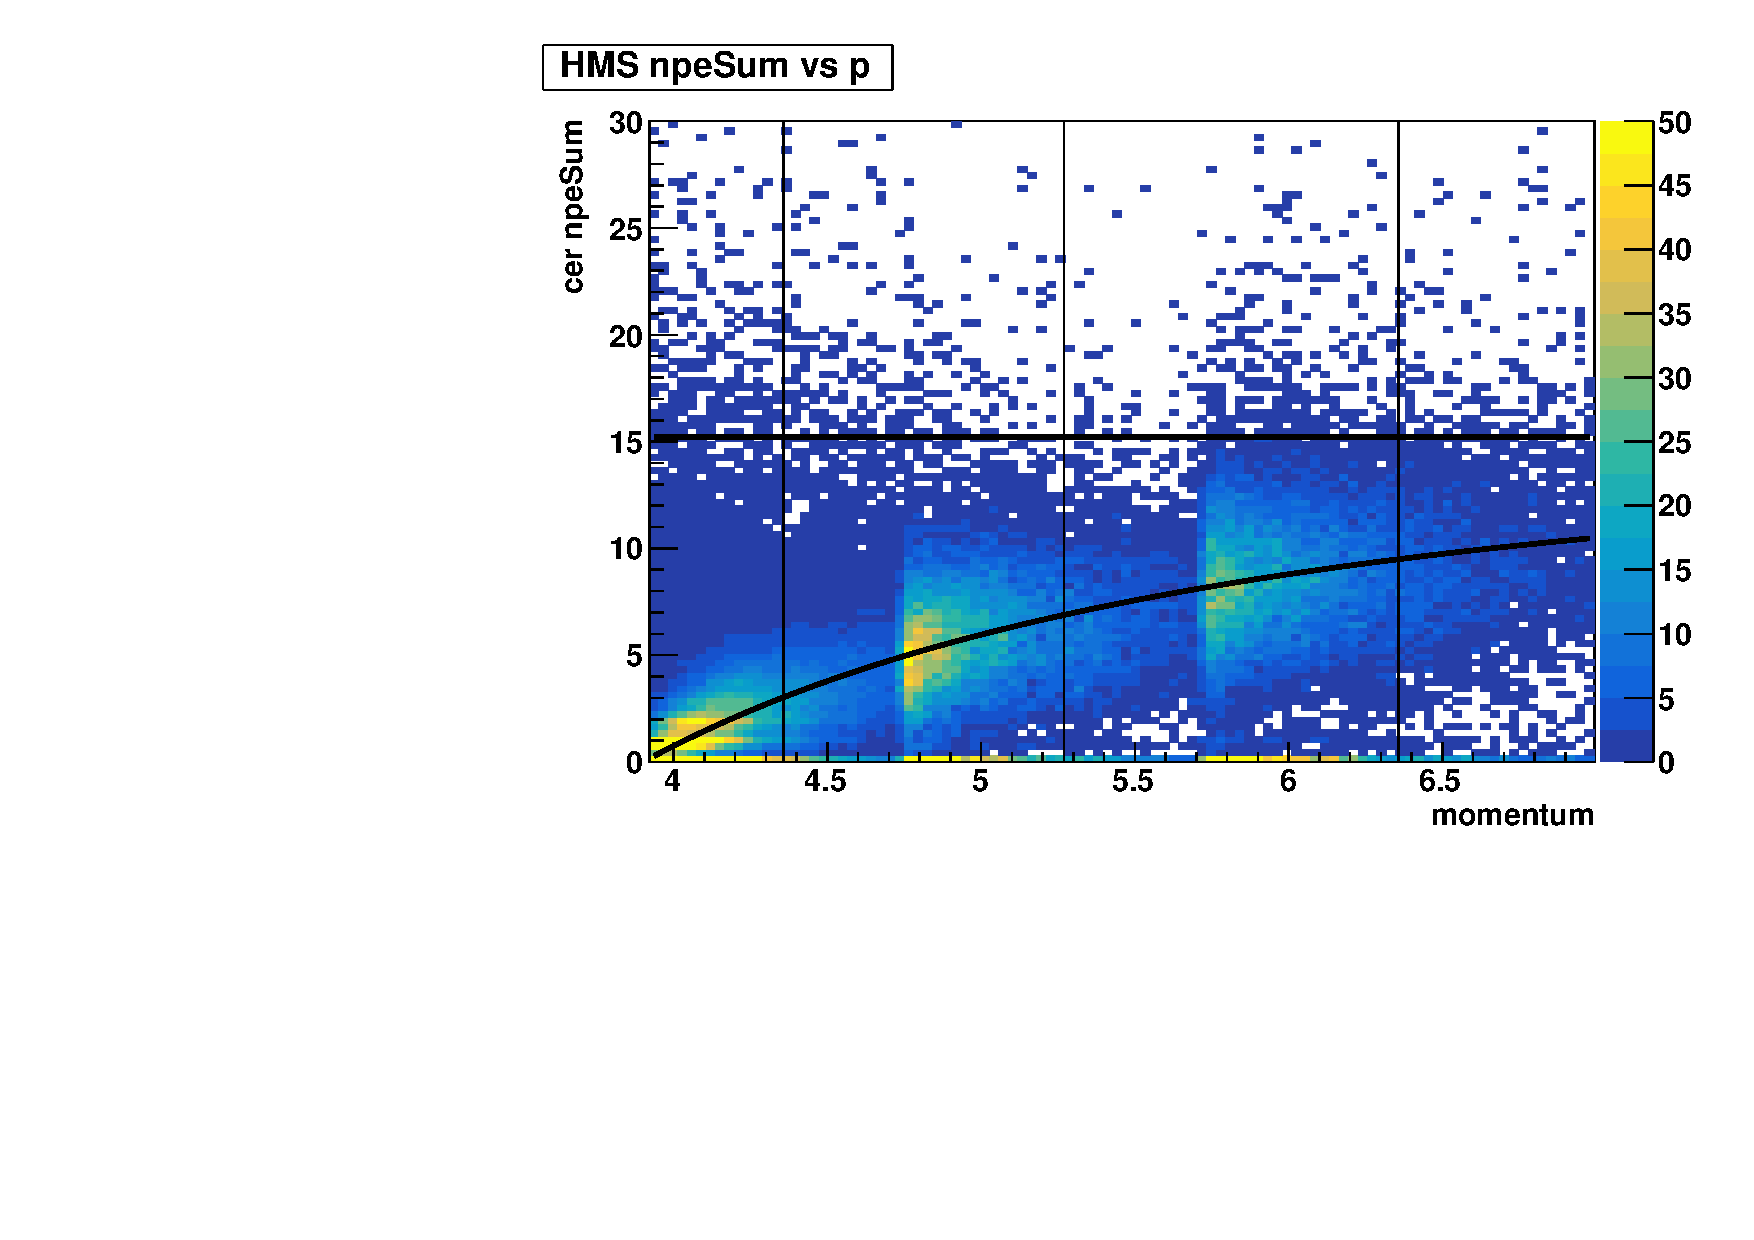
\includegraphics[width = 0.7\textwidth]{results/pid/all_npeSum_p_32.pdf}
\\
HMS Cherenkov detector has pion threshold 3.8, which is not a good pion rejector. To select good electron sample, I use cernpe greater than 12.  
\end{frame}
\begin{frame}{efficiency with cut}
  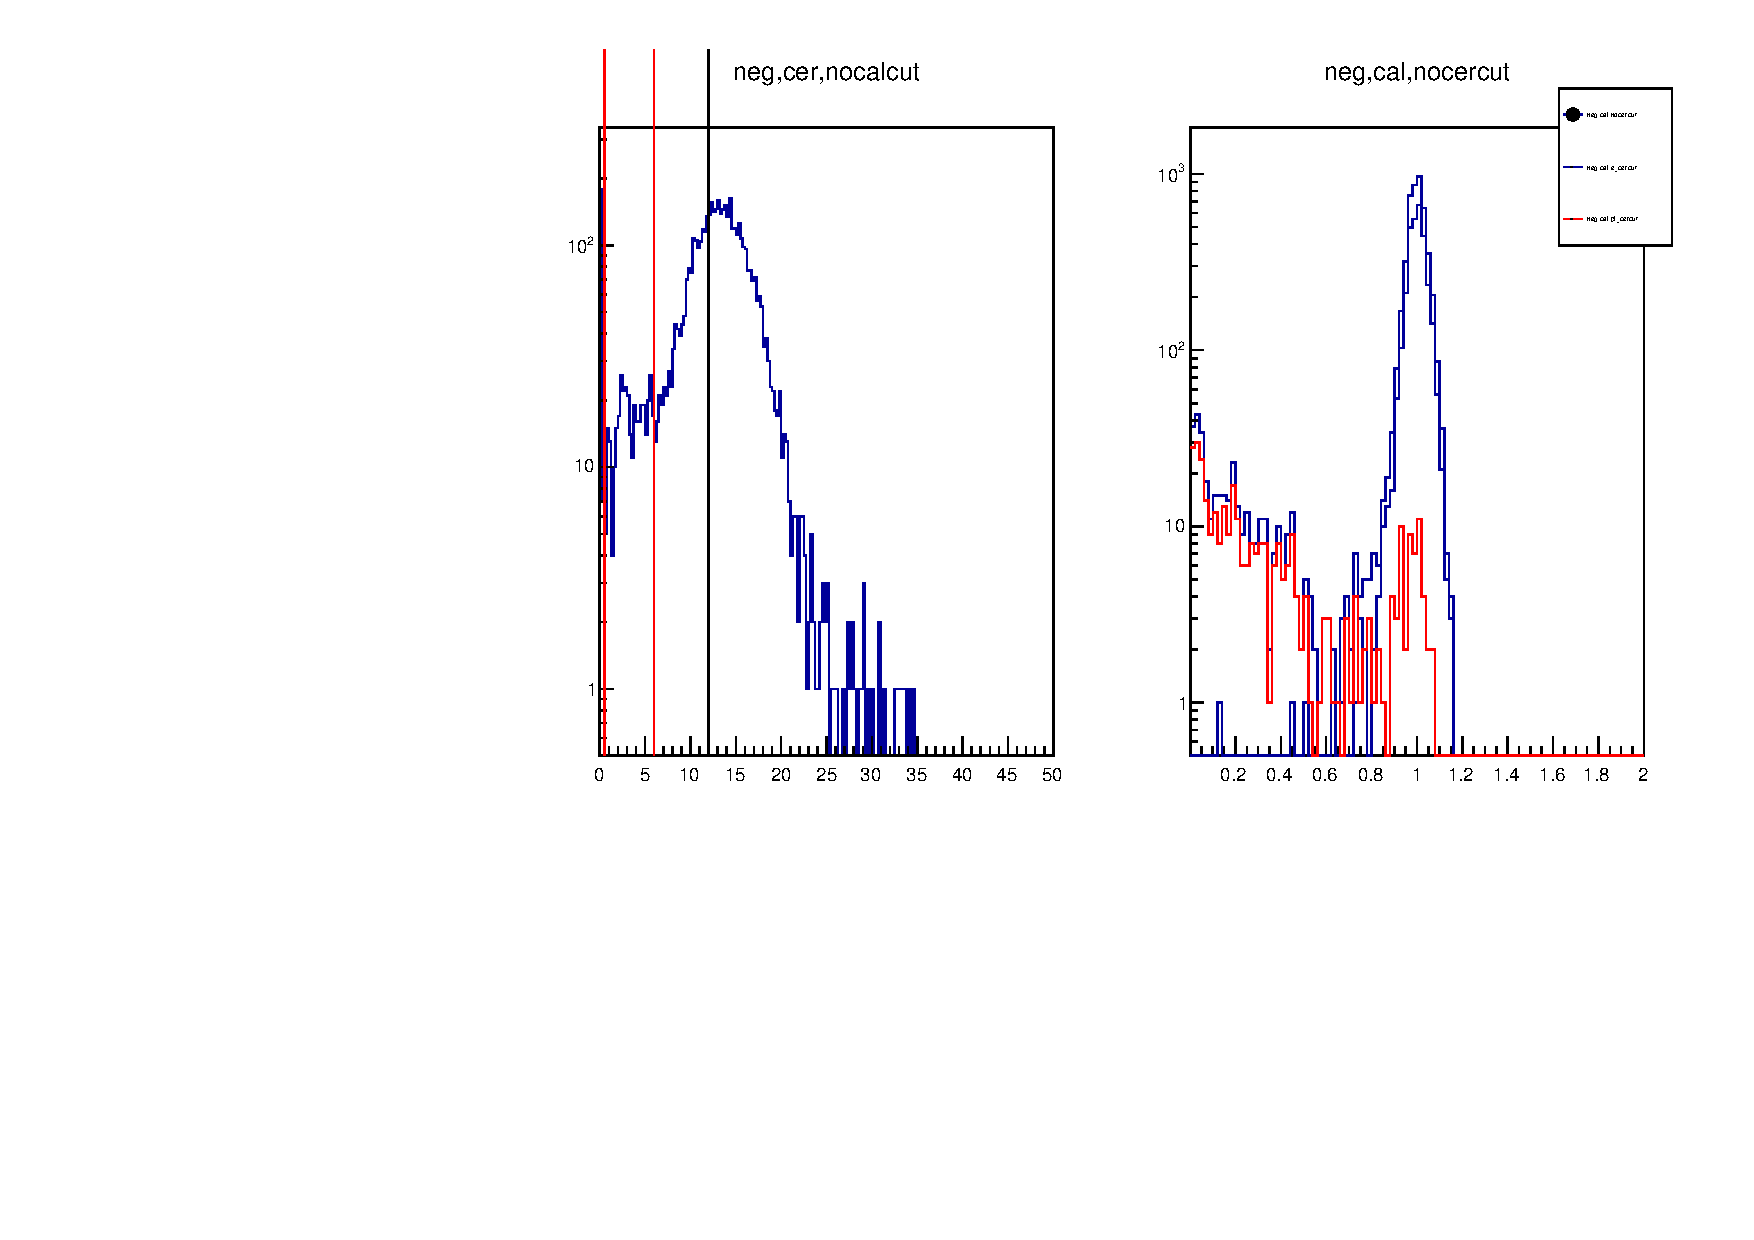
\includegraphics[width = 0.6\textwidth]{results/pid/cal_DE_6524.pdf}
  \\
  RunNumber 6524, in run group 360, momentum 4.736, neg
  \\
  $$cal\_eff = \frac{e\_did[cer\_cut \& cal\_cuts]}{e\_sample[cer\_cut]}$$
\end{frame}
\begin{frame}{ efficiency with cut}
  \begin{columns}
    \begin{column}[T]{0.5\textwidth}
  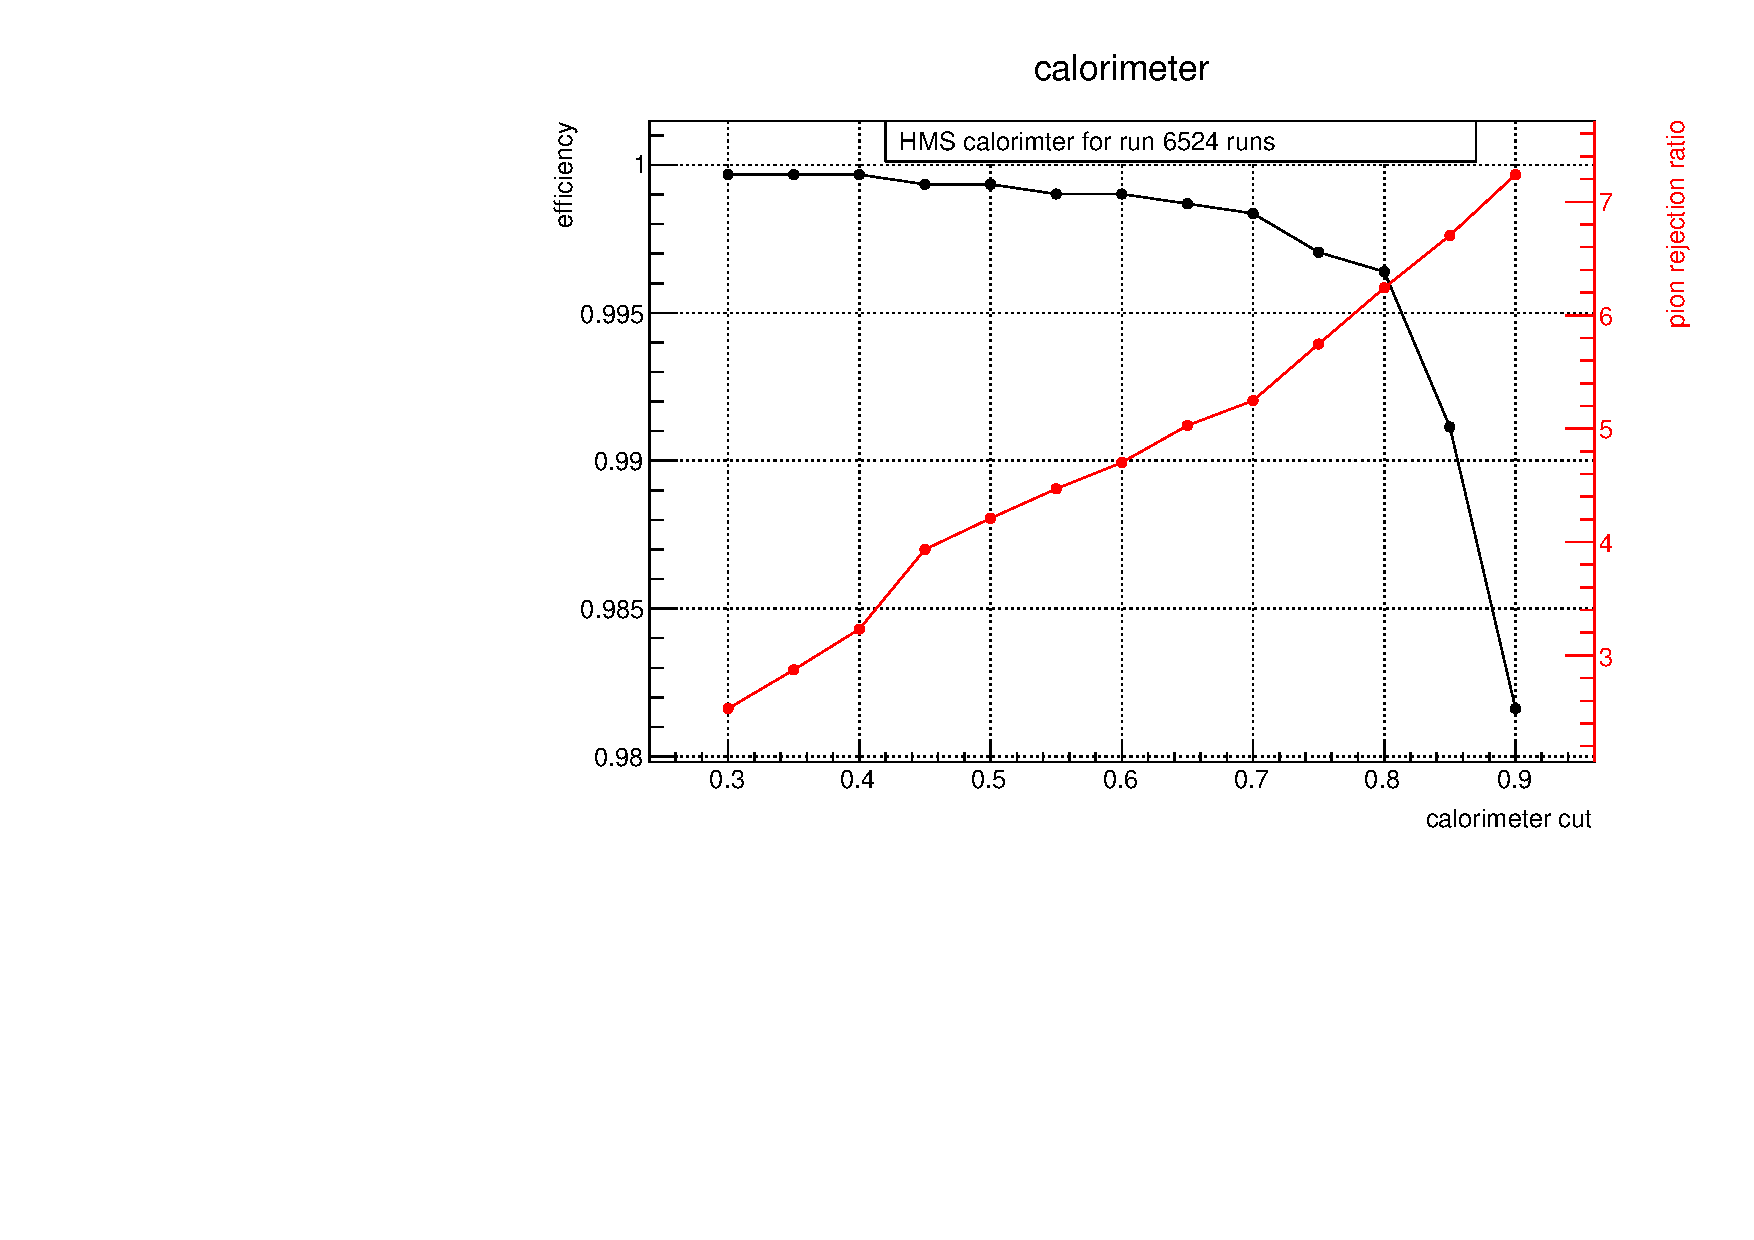
\includegraphics[width = 0.8\textwidth]{results/pid/HMS_cal_6524.pdf}
\end{column}
\begin{column}[T]{0.5\textwidth}
  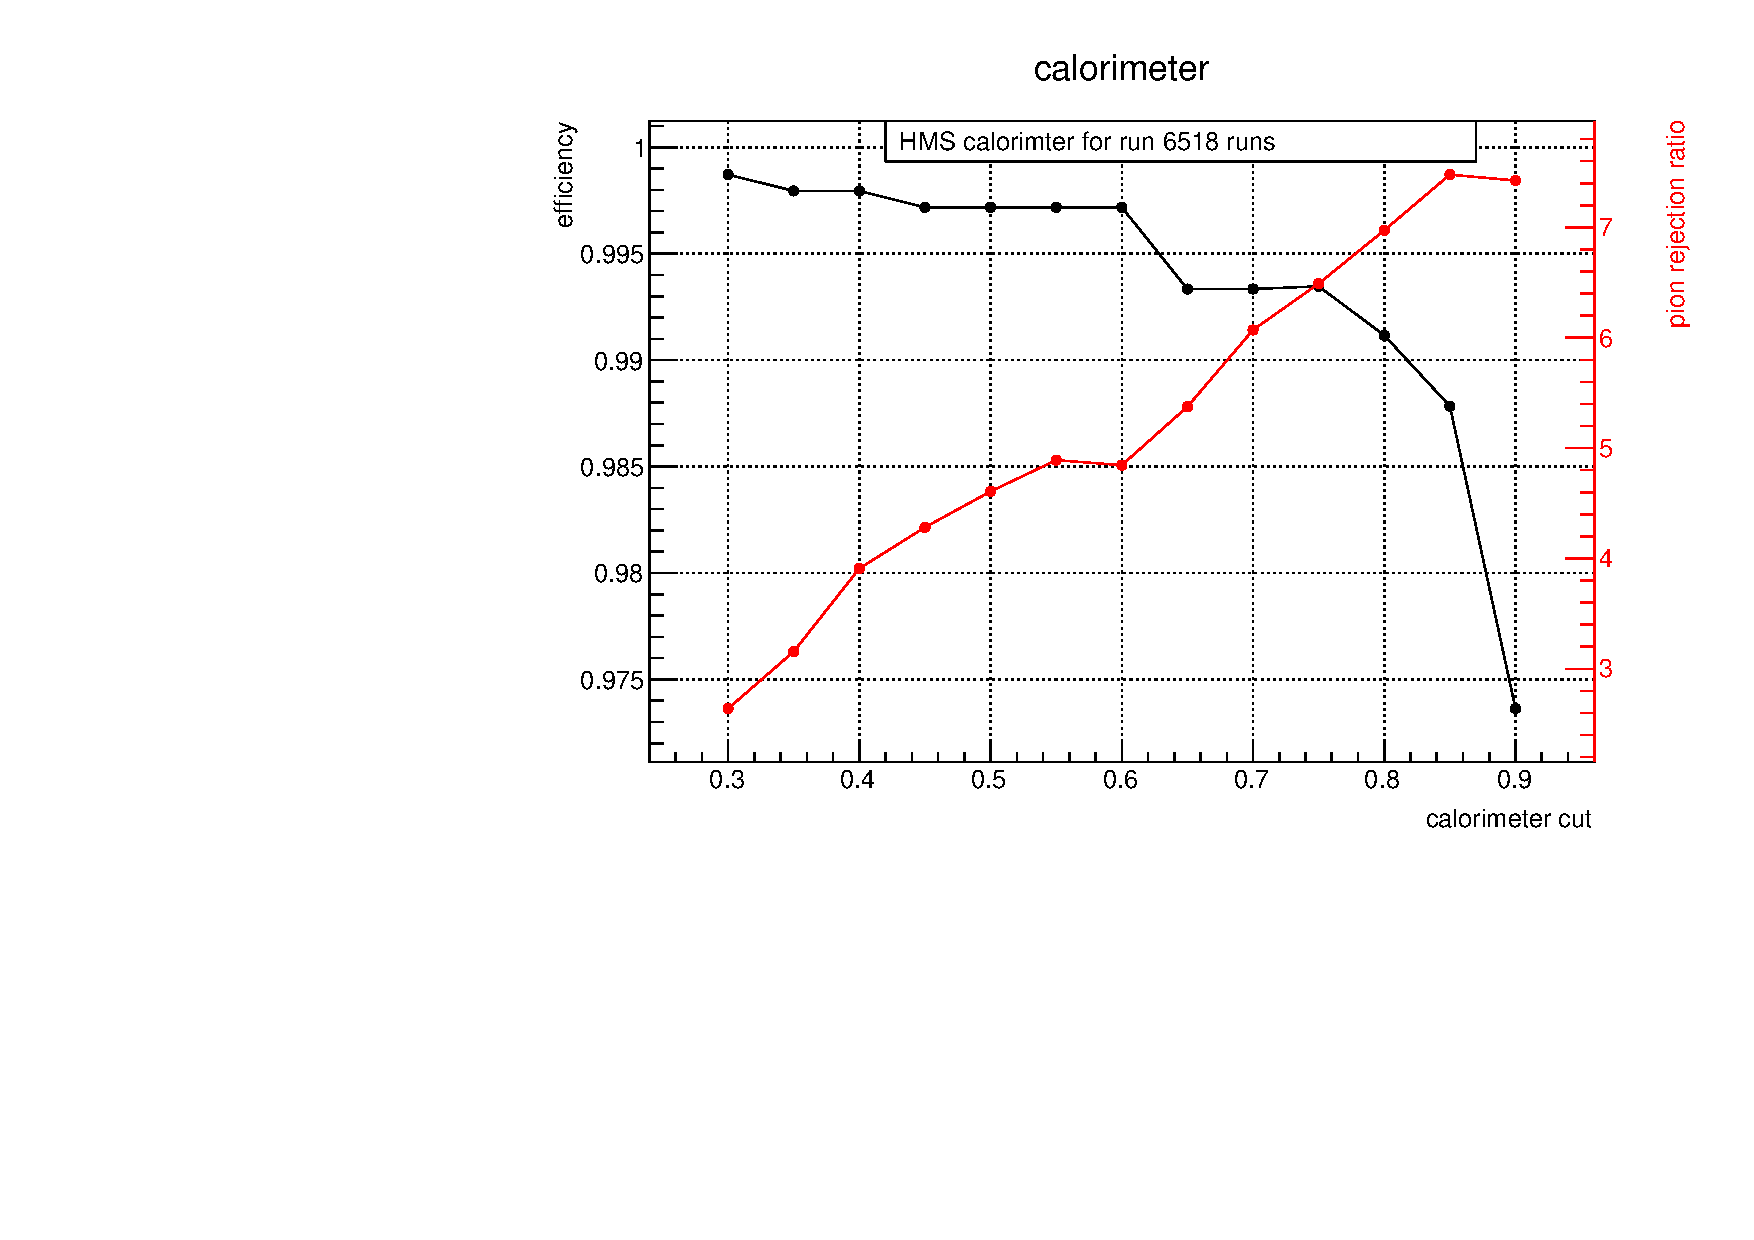
\includegraphics[width = 0.8\textwidth]{results/pid/HMS_cal_6518.pdf}
\end{column}
\end{columns}
  \\
  left is neg run 6524,right is pos run 6518, in run group 360, momentum 4.736
\end{frame}
\begin{frame}{HMS Detector efficiency verse momentum}
  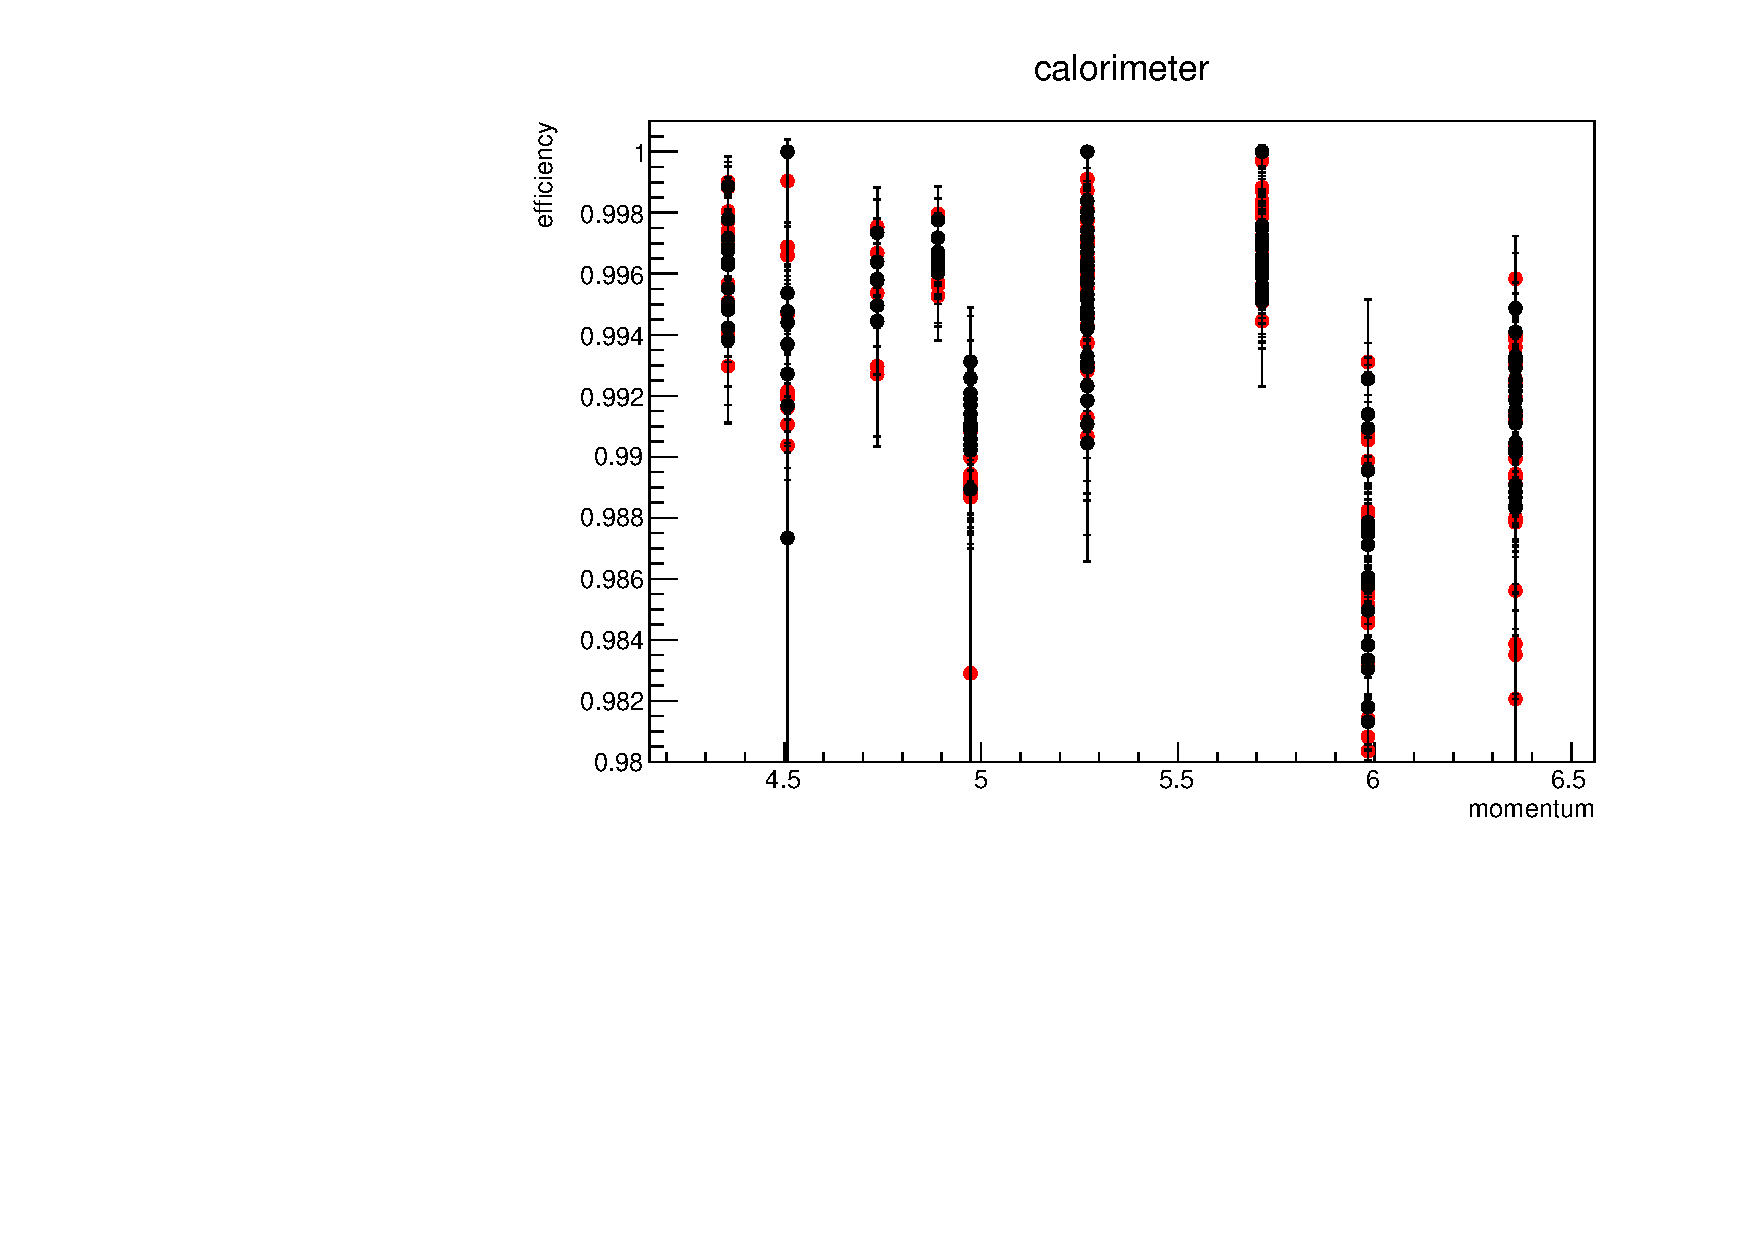
\includegraphics[width = 0.8\textwidth]{results/pid/HMS_cal_DE_momentum.pdf}
\end{frame}
\begin{frame}{HMS Detector efficiency verse RunNumber}
  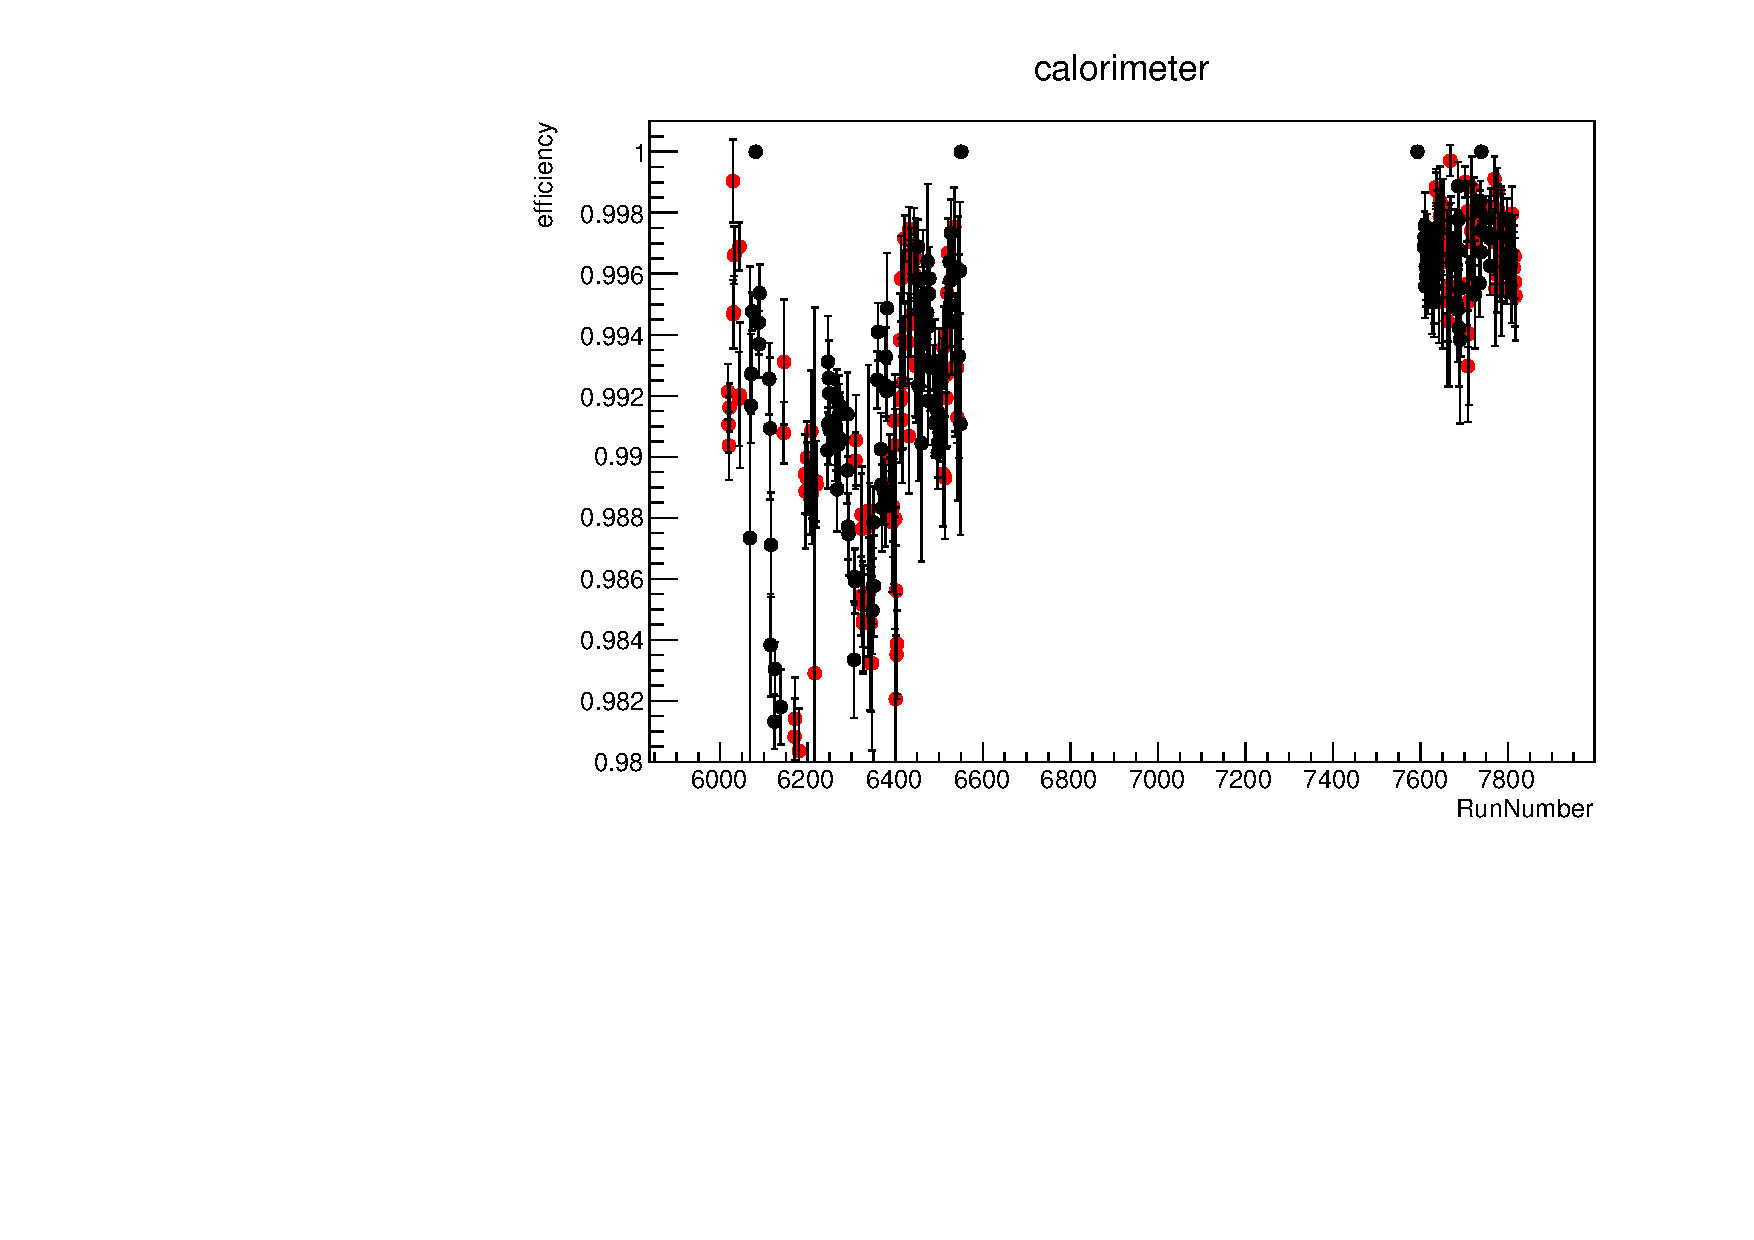
\includegraphics[width = 0.8\textwidth]{results/pid/HMS_cal_DE_RunNumber.pdf}
\end{frame}
\begin{frame}{HMS Detector efficiency verse RunGroup}
  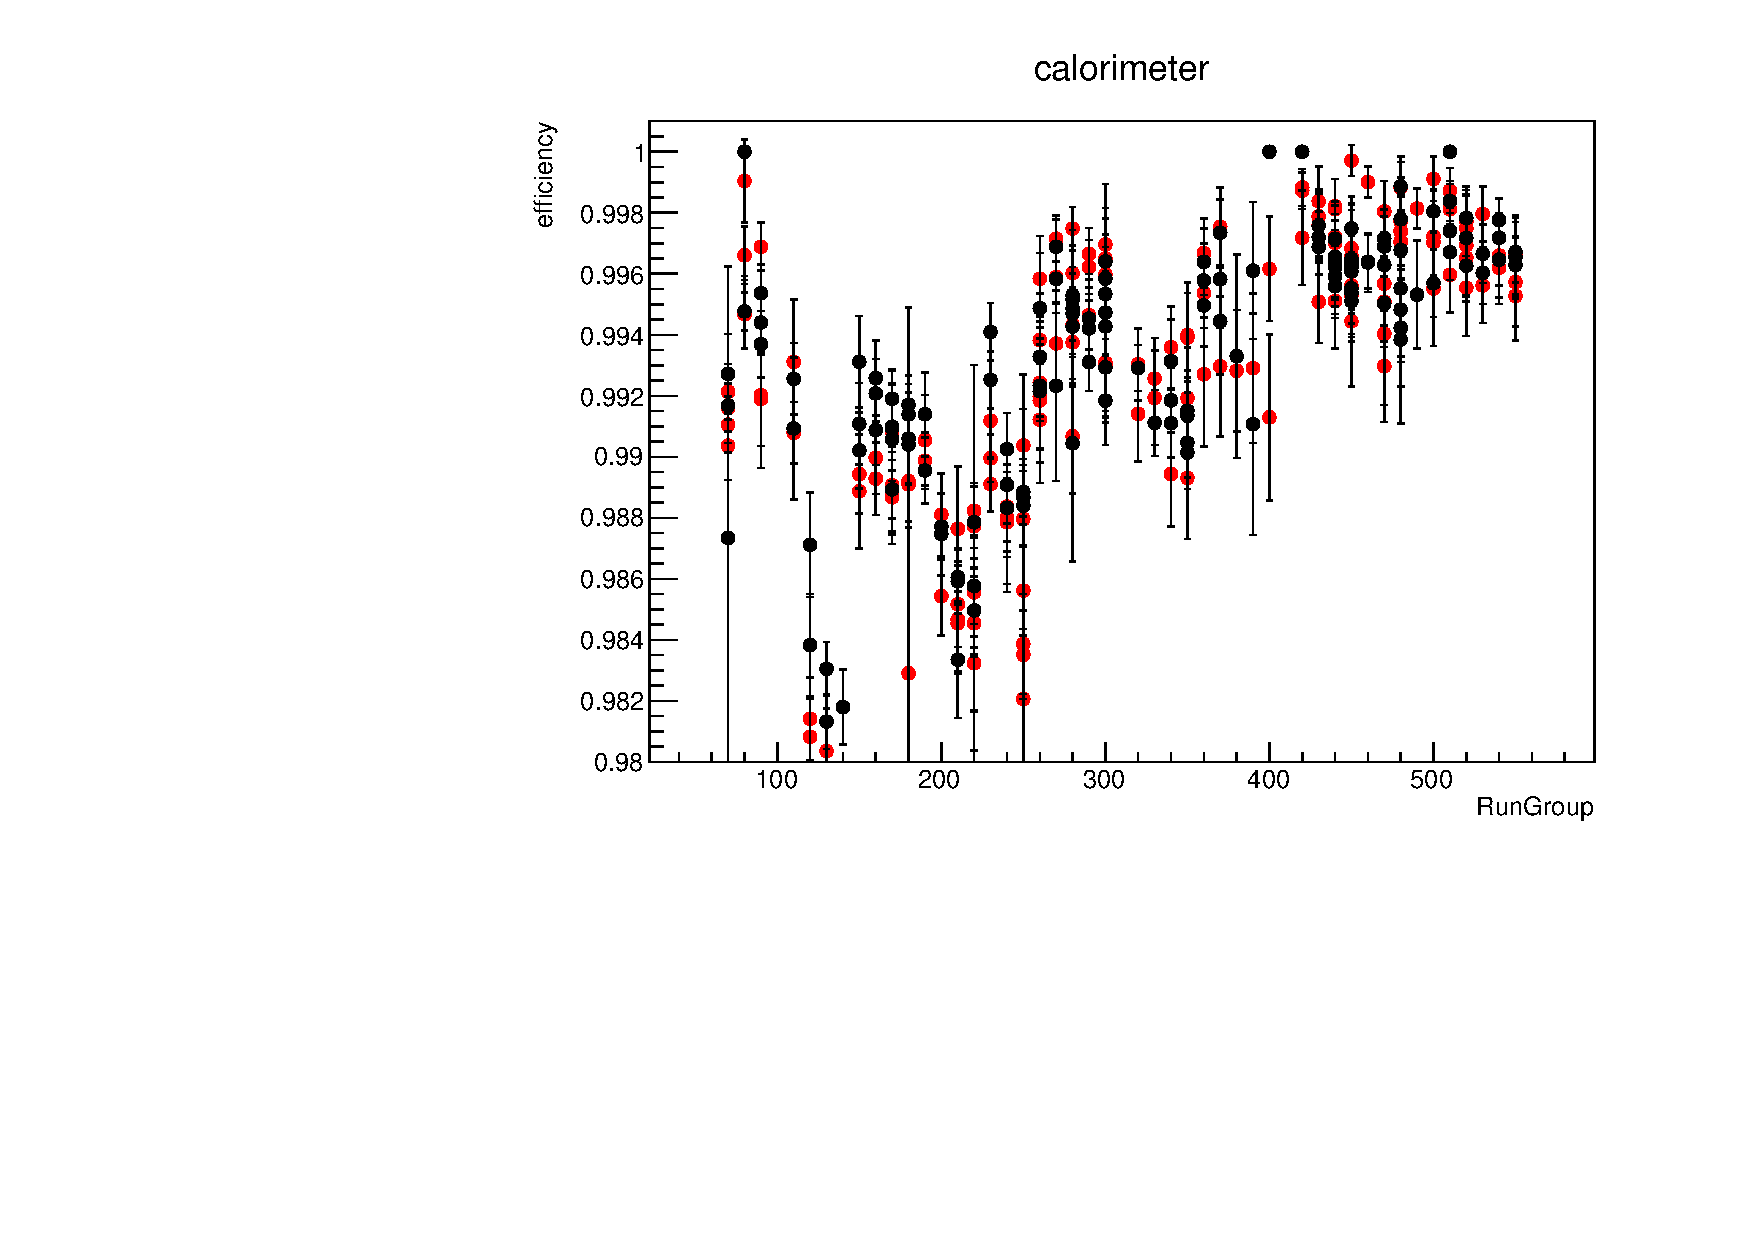
\includegraphics[width = 0.8\textwidth]{results/pid/HMS_cal_DE_RunGroup.pdf}
\end{frame}
\begin{frame}{efficiency with cut}
  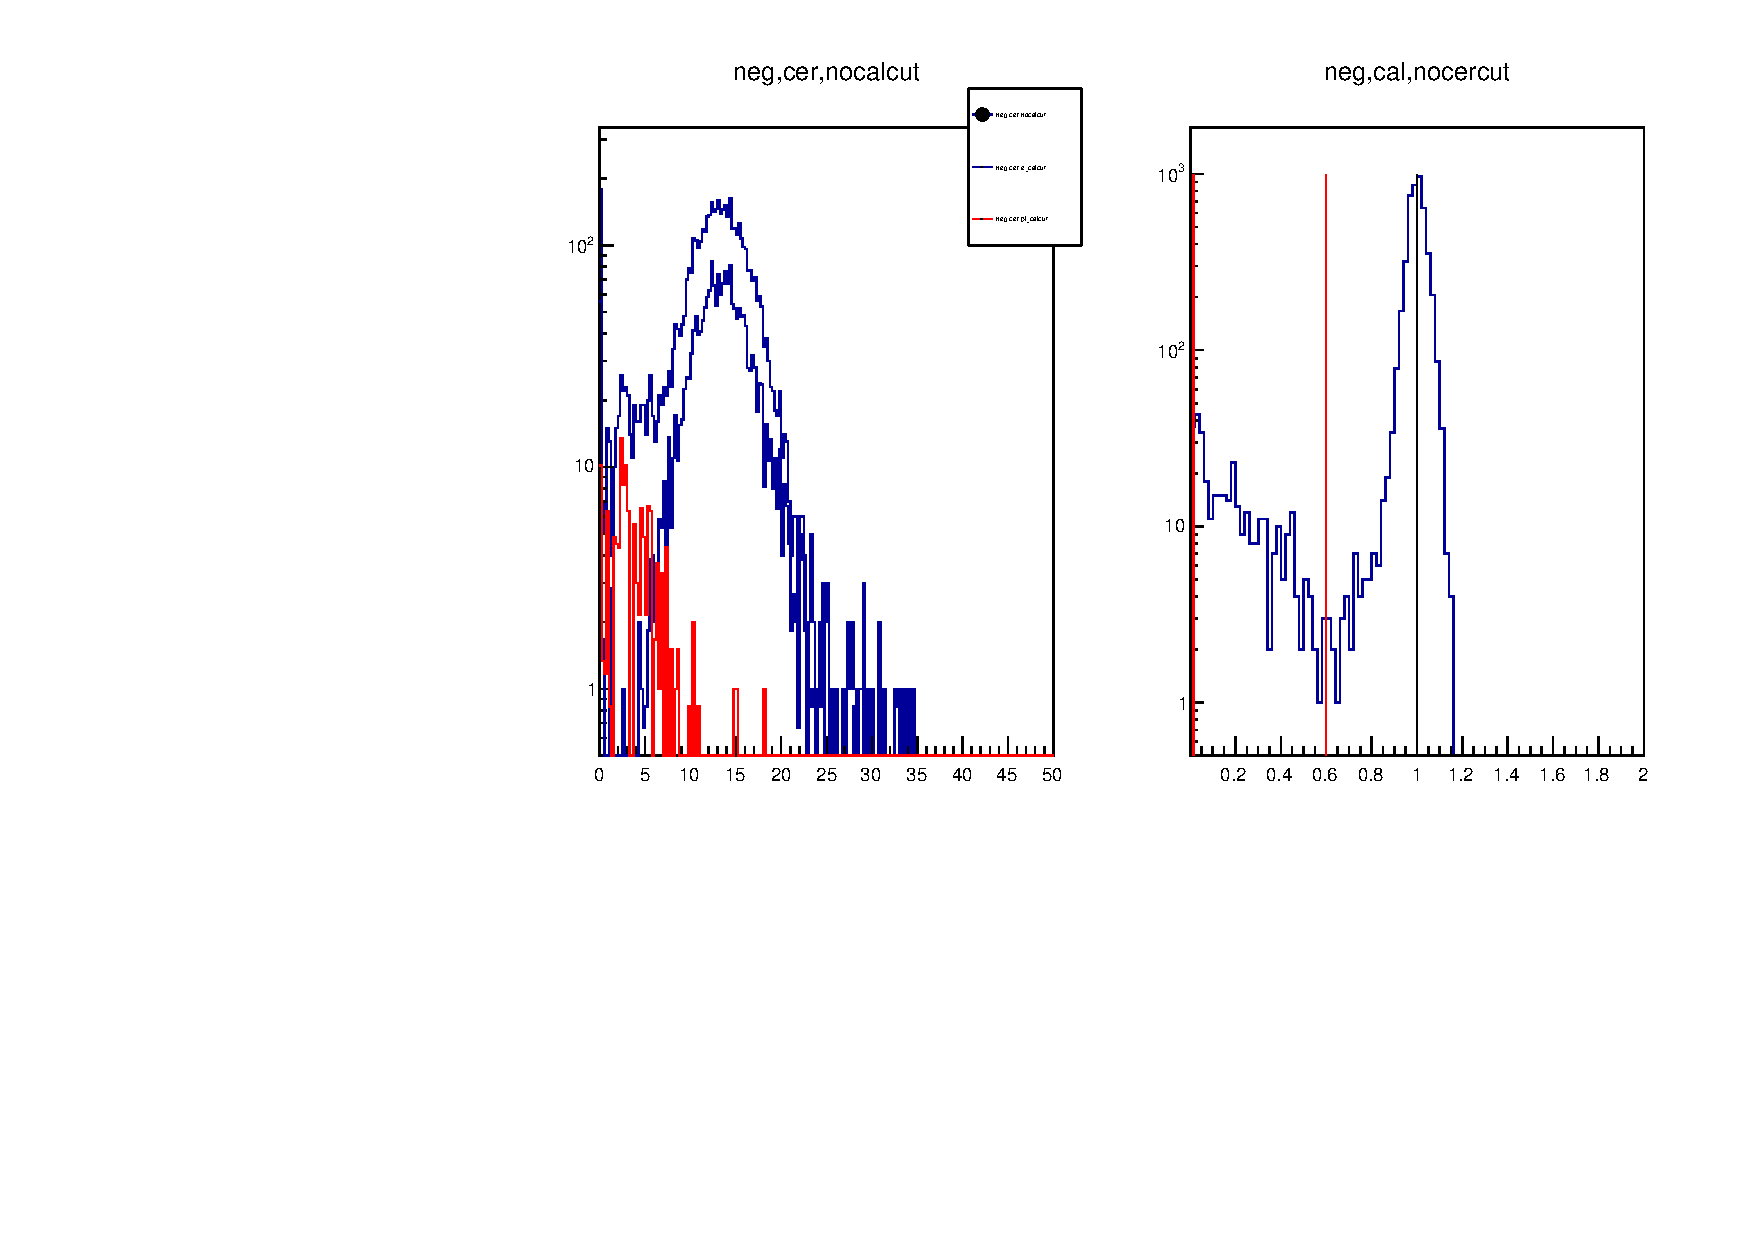
\includegraphics[width = 0.6\textwidth]{results/pid/cer_DE_6524.pdf}
  \\
  RunNumber 6524, in run group 360, momentum 4.736, neg, cal cut greater than 1
  \\
  $$cer\_eff = \frac{e\_did[cal\_cuts \& cer\_cuts]}{e\_sample[cal\_cut]}$$
\end{frame}
\begin{frame}{efficiency with cut}
  \begin{columns}
    \begin{column}[T]{0.5\textwidth}
  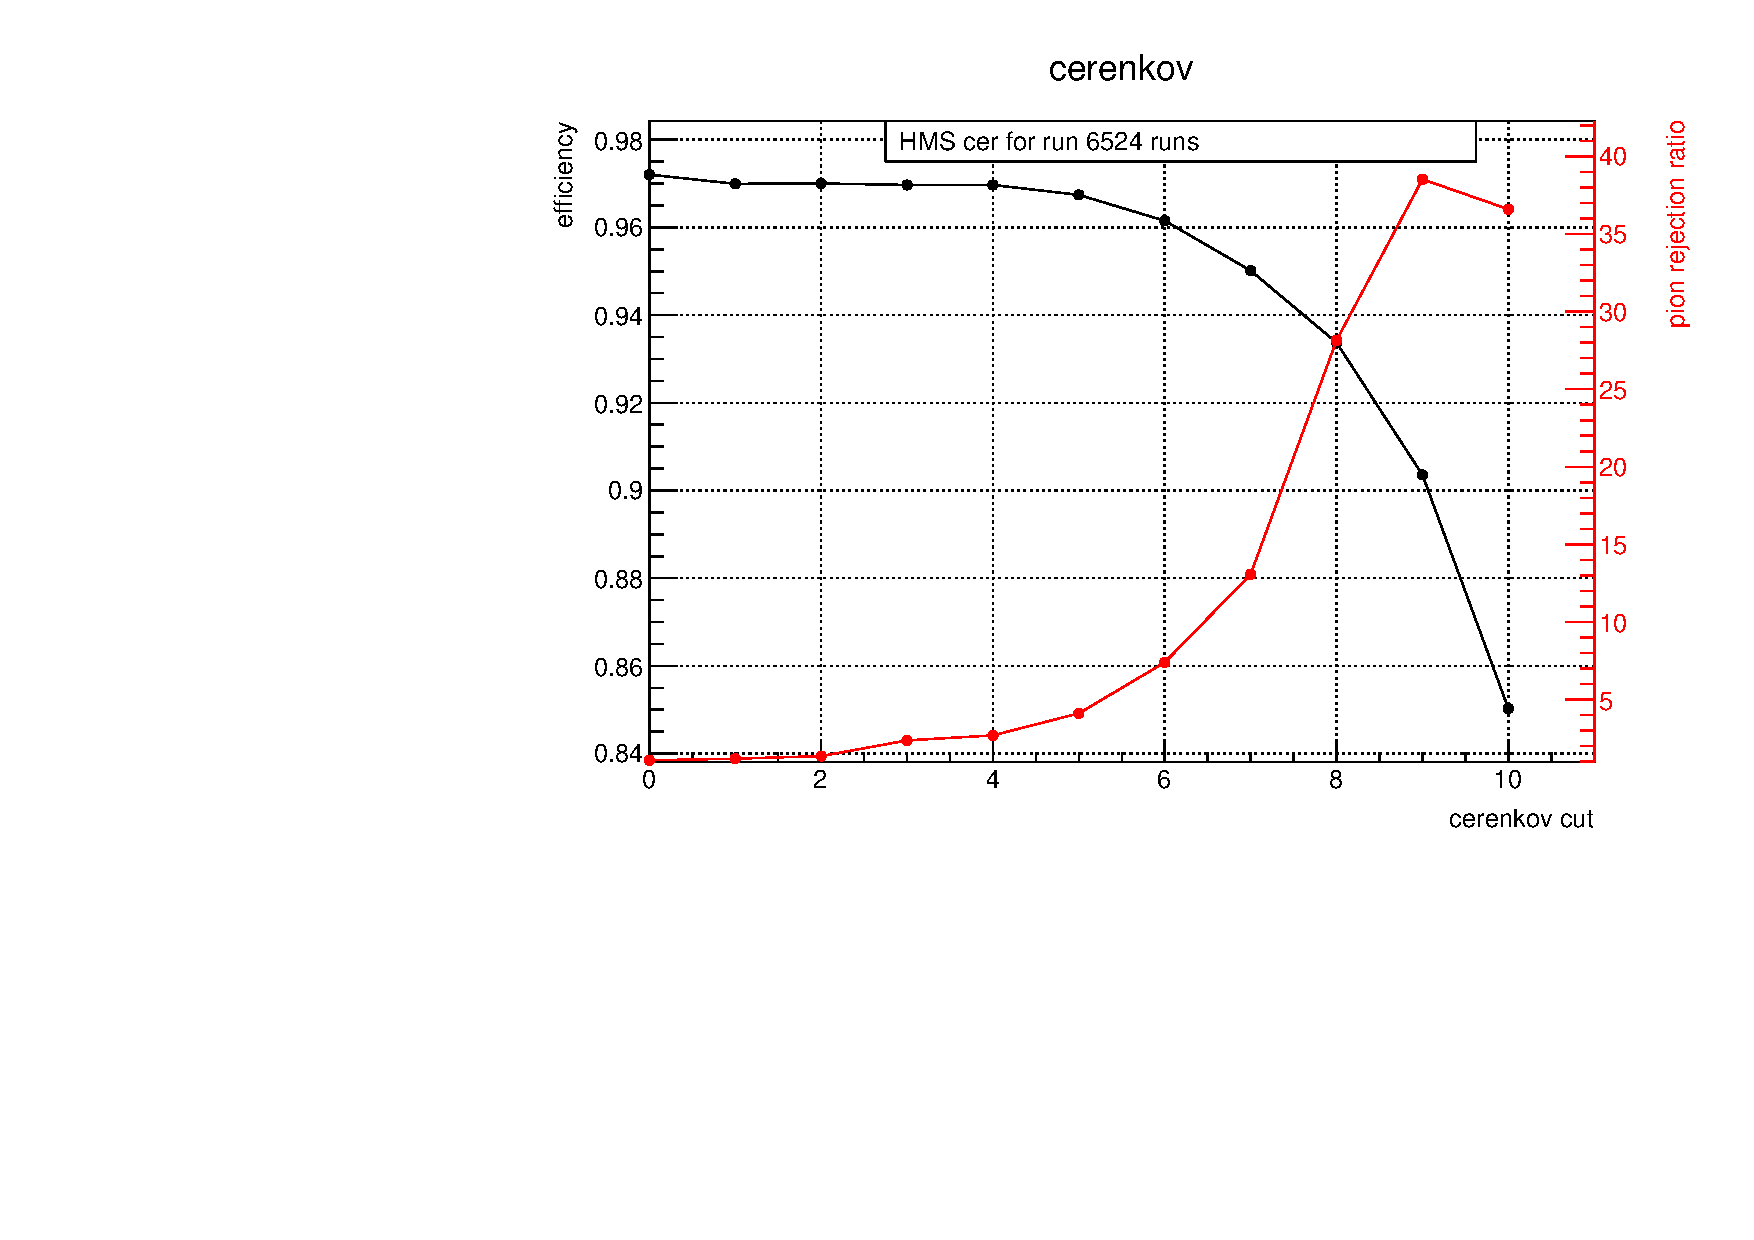
\includegraphics[width = 0.8\textwidth]{results/pid/HMS_cer_6524.pdf}
\end{column}
\begin{column}[T]{0.5\textwidth}
  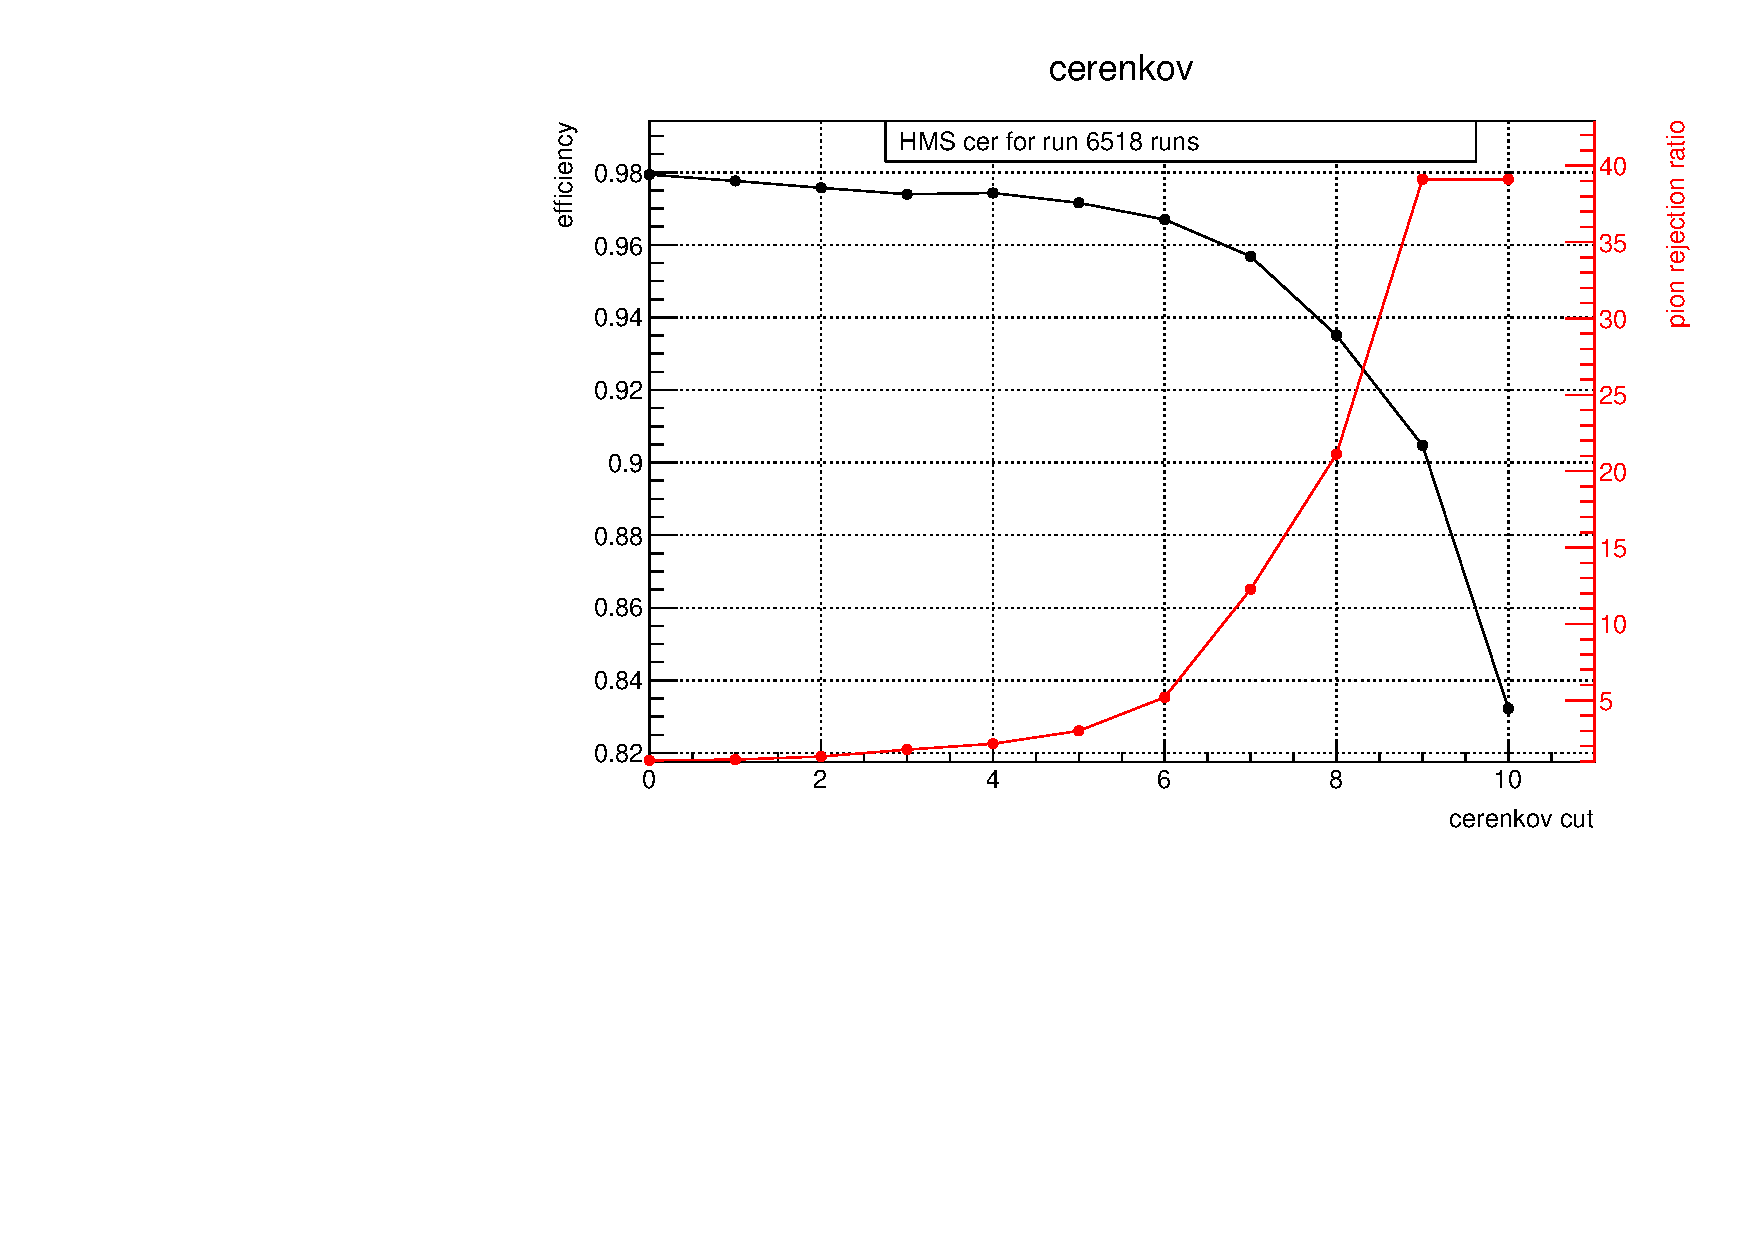
\includegraphics[width = 0.8\textwidth]{results/pid/HMS_cer_6518.pdf}
\end{column}
\end{columns}
  left is neg run 6524,right is pos run 6518, in run group 360, momentum 4.736
  
\end{frame}
\begin{frame}{HMS Detector efficiency verse momentum}
  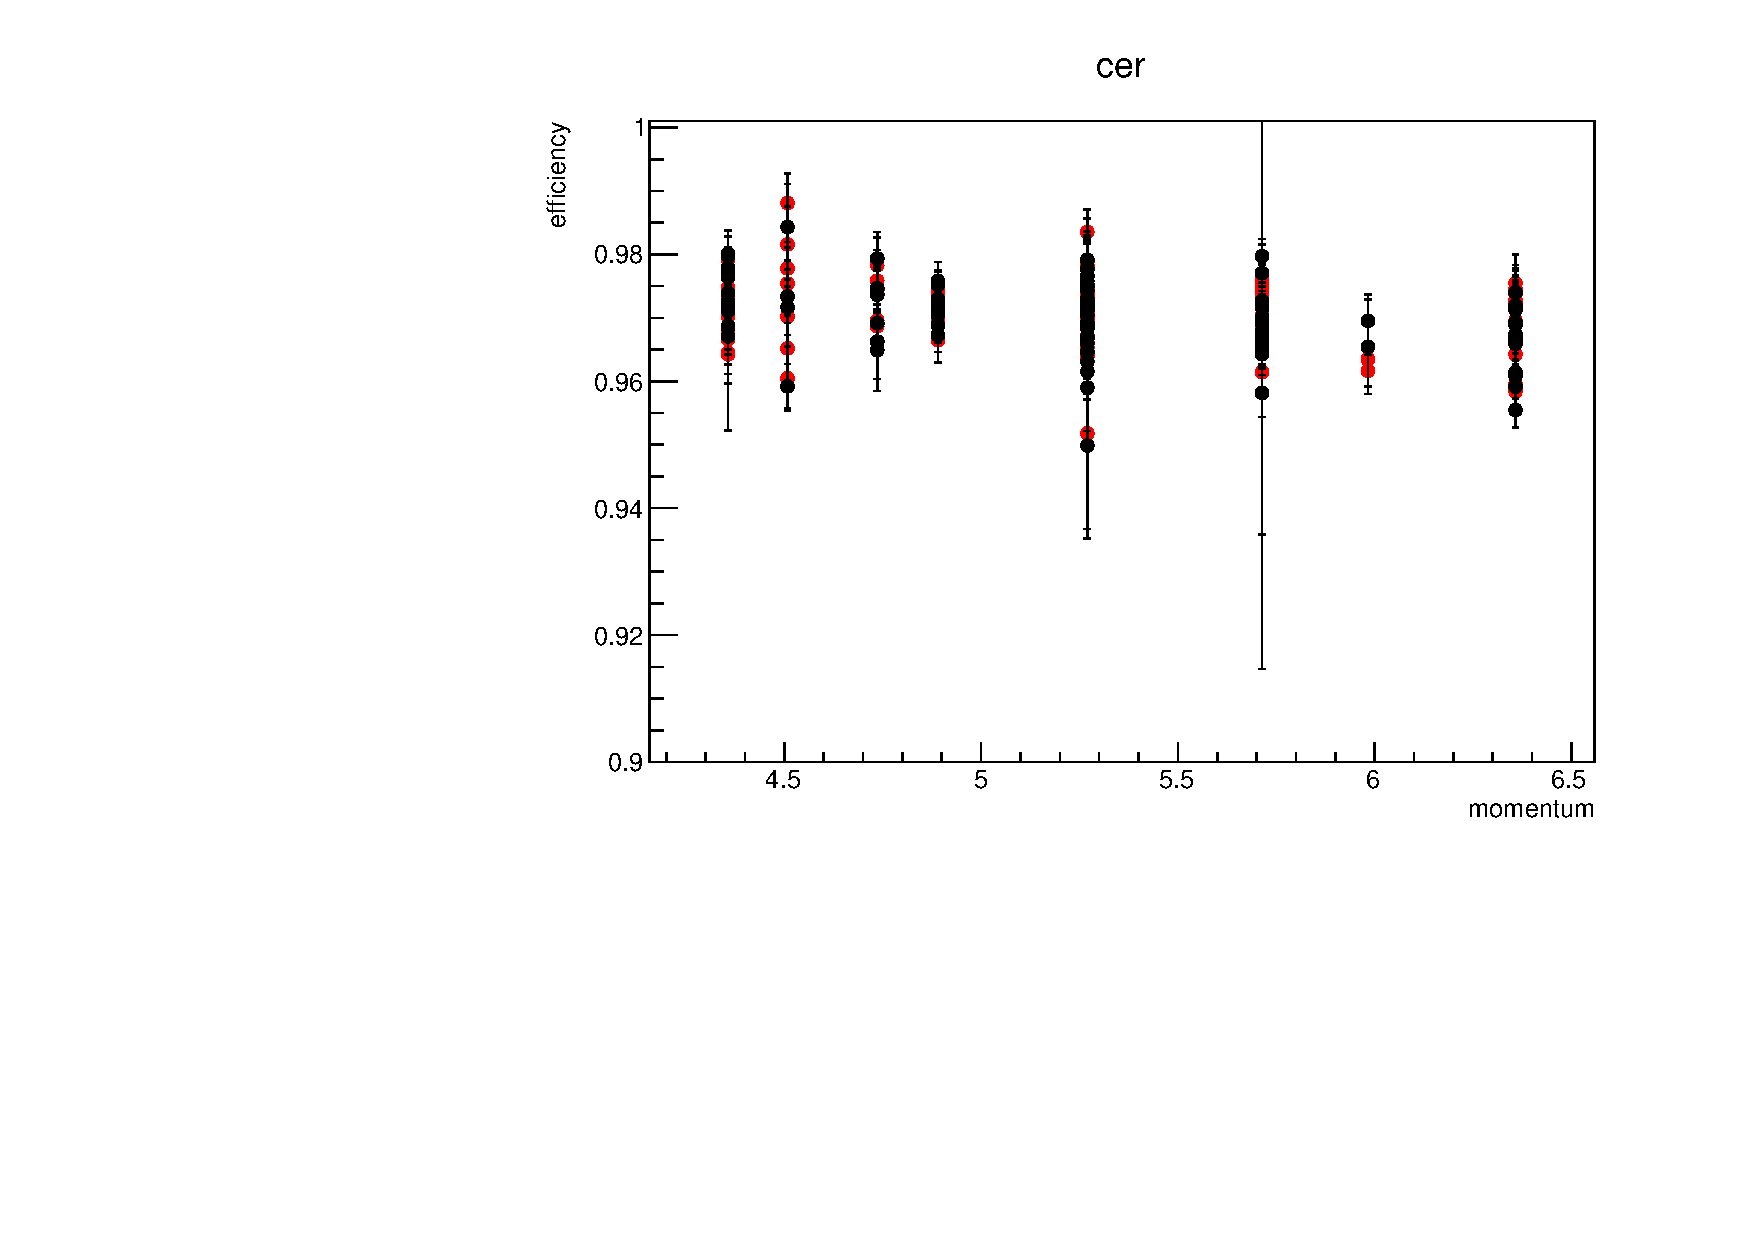
\includegraphics[width = 0.8\textwidth]{results/pid/HMS_cer_DE_momentum.pdf}
\end{frame}
\begin{frame}{HMS Detector efficiency verse RunNumber}
  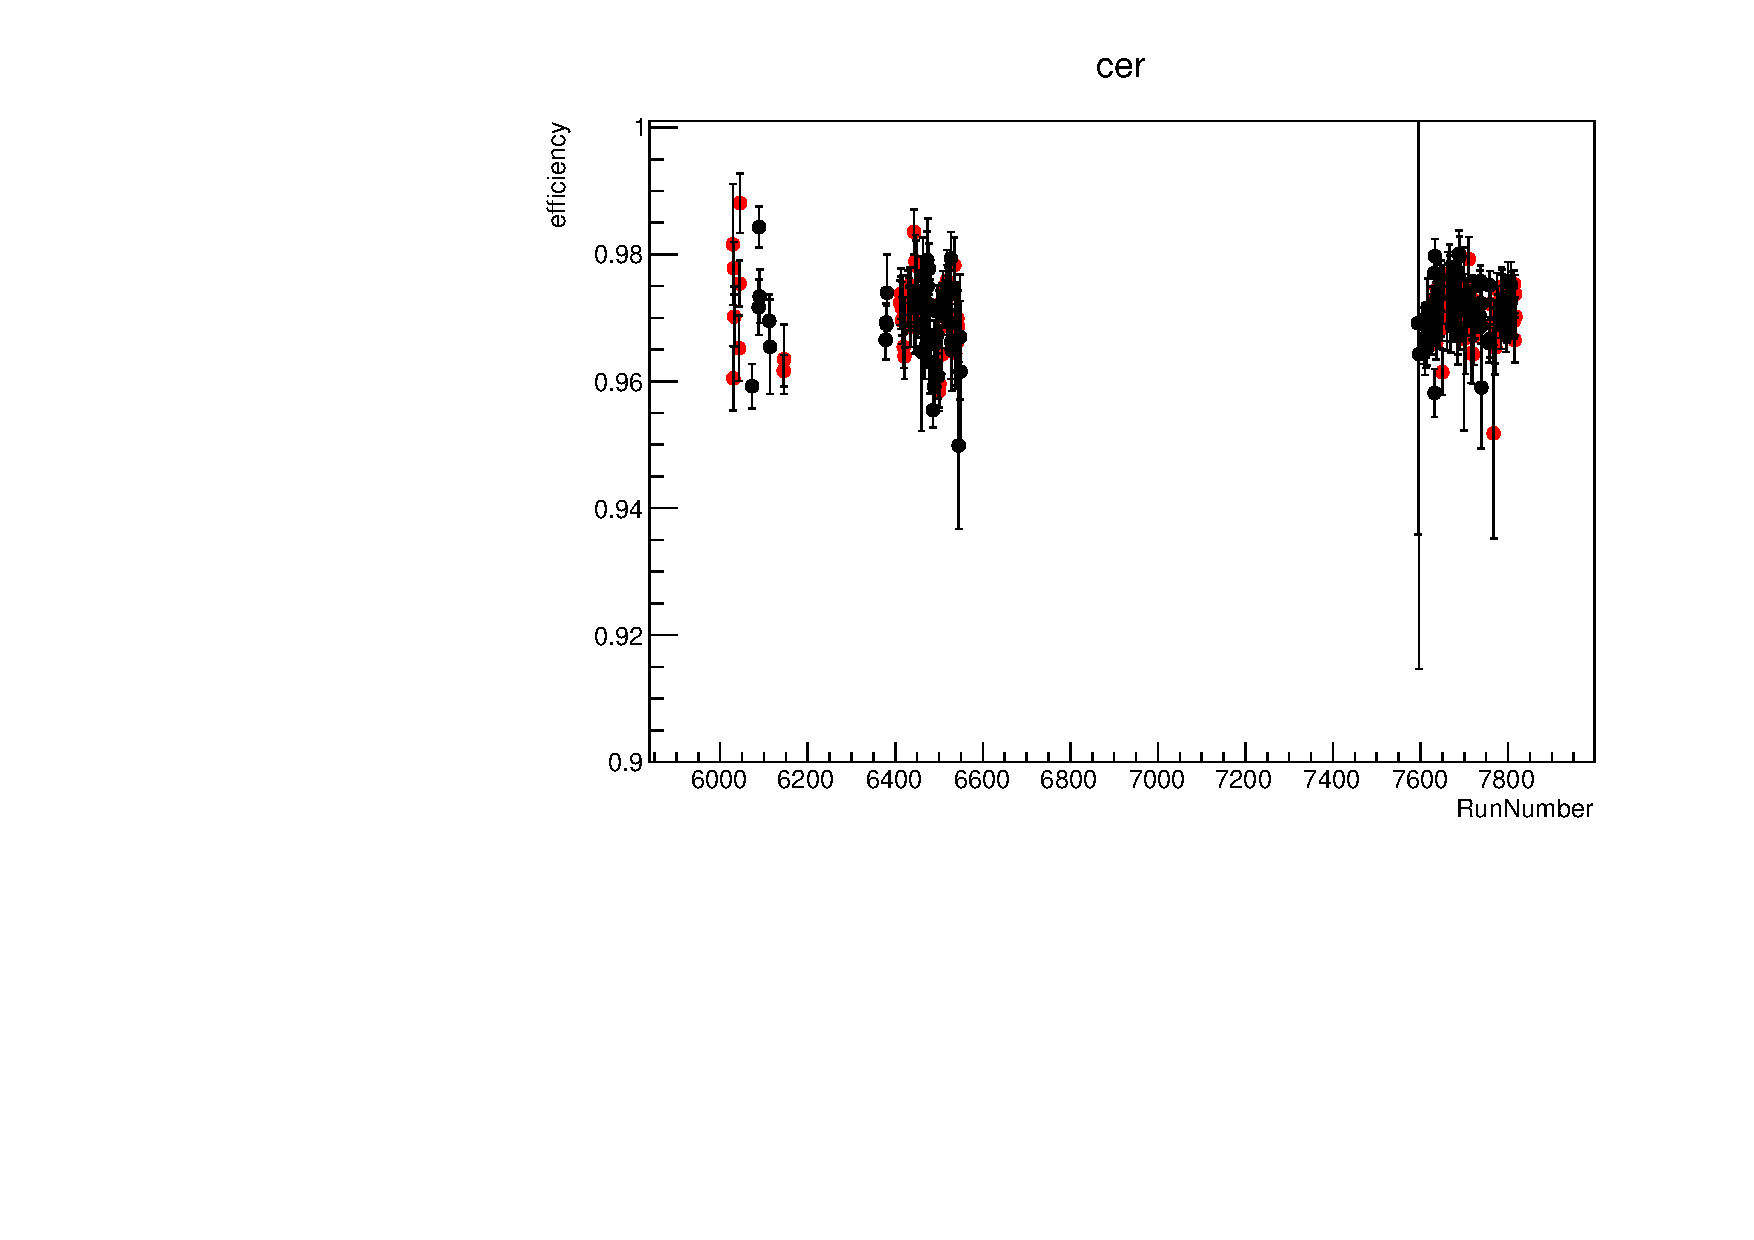
\includegraphics[width = 0.8\textwidth]{results/pid/HMS_cer_DE_RunNumber.pdf}
\end{frame}
\begin{frame}{HMS Detector efficiency verse RunGroup}
  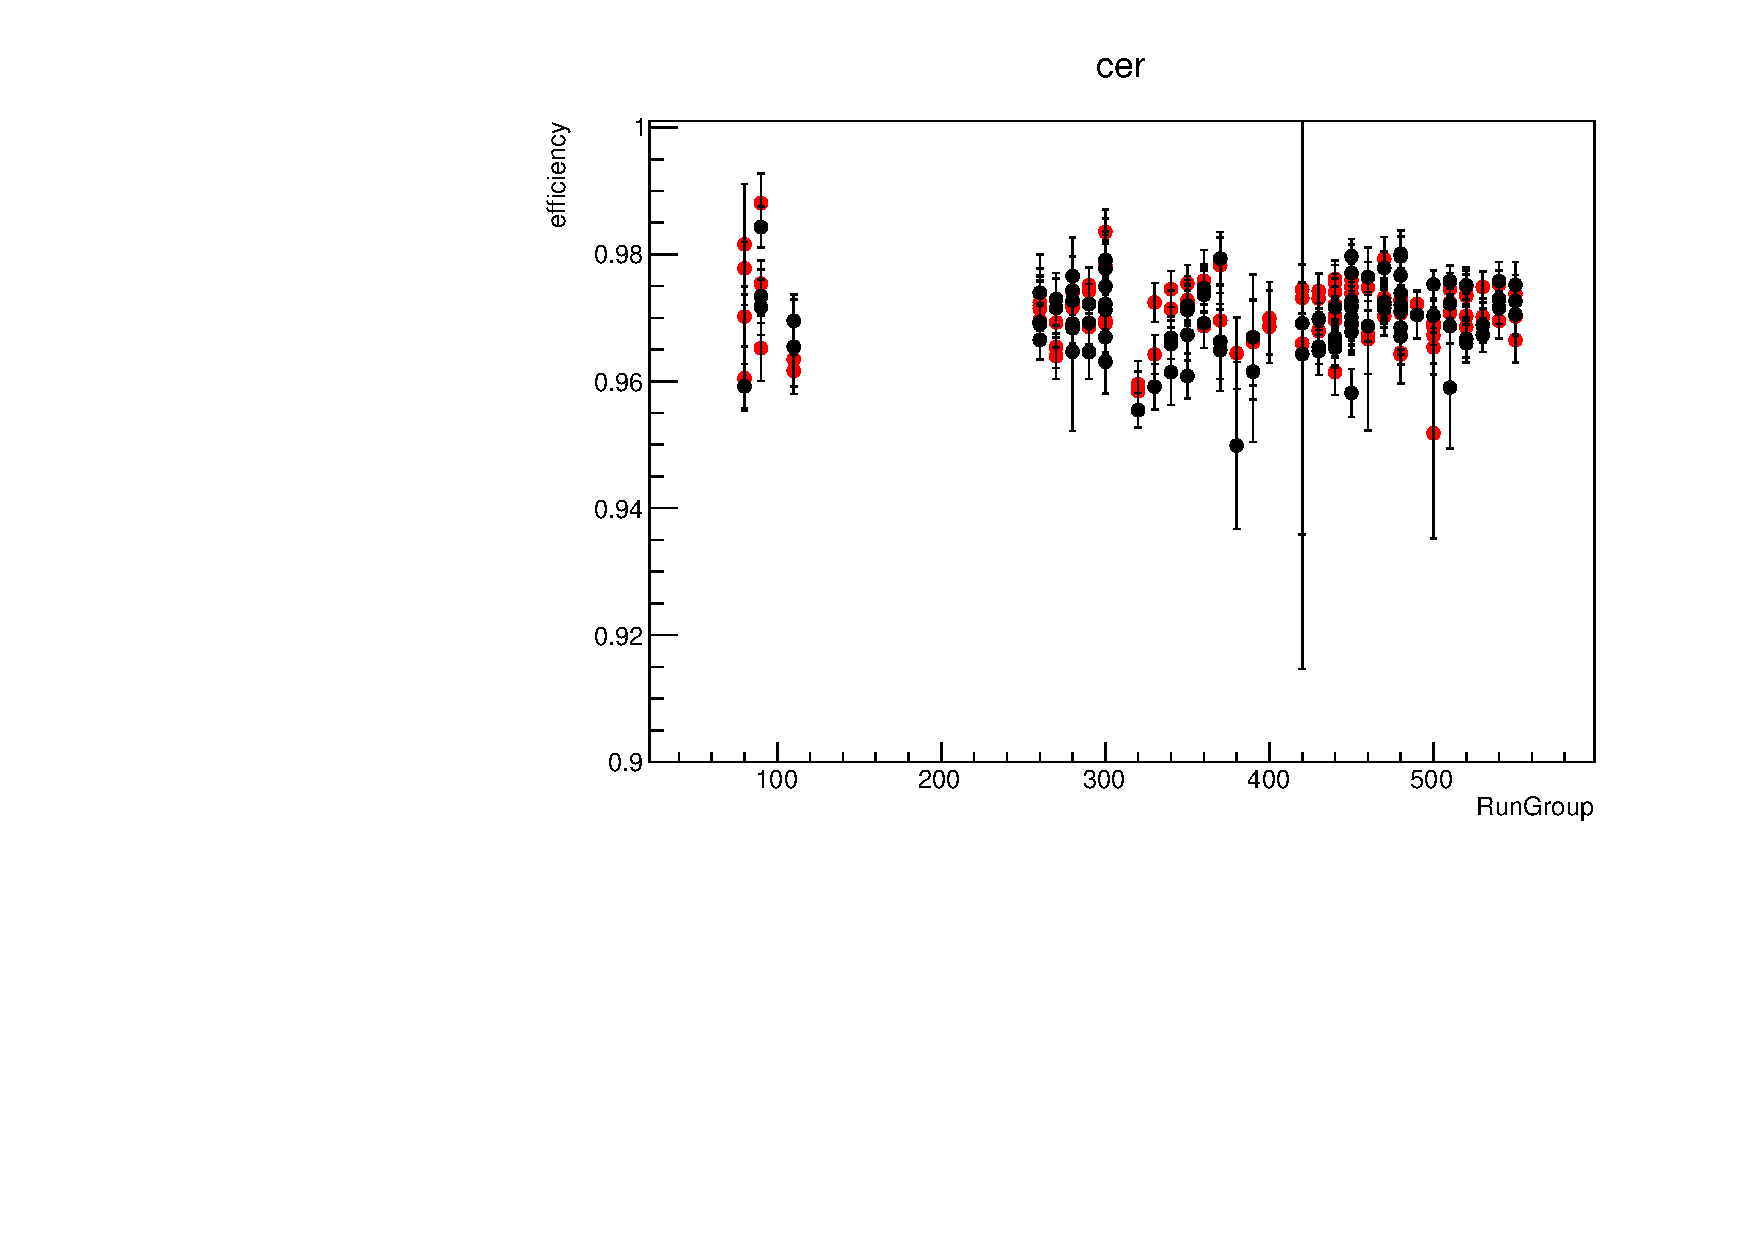
\includegraphics[width = 0.8\textwidth]{results/pid/HMS_cer_DE_RunGroup.pdf}
\end{frame}
\begin{frame}{SHMS pion arm}
  \begin{block}{Basic cuts}
    cointime:2.5(fall)/1.5(spring) \\
    HMS(SHMS) delta:-8,8(-10,20) \\
    HMS(SHMS) acceptance constrain \\
    HMS e cut \\
    accidental background: 6 peaks \\
  \end{block}
  \begin{columns}
    \begin{column}[T]{0.5\textwidth}
     \begin{block}{SHMS Calorimeter}
       Aerogel Cherenkov cut: 2 \\
       rftime cut: 0.5,1.5 \\ 
       Calorimeter cut: varies 
     \end{block}
   \end{column}
   \begin{column}[T]{0.5\textwidth}
     \begin{block}{SHMS aerogel Cherenkov}
       Aerogel Cherenkov cut: varies \\
       rftime cut: 0.5,1.5 \\ 
       Calorimeter cut: 0.05,0.85
       \end{block}
     \end{column}
   \end{columns}
  %\begin{center}
  %  \begin{tabular}{|c|c|c|c|c|c|}
  %    \hline
  %    Cuts & HMS cal &HMS cer &  SHMS cal & SHMS aero & SHMS rf \\
  %    \hline
  %    cointime & 1.5/2.5 & same & same & same & same\\
  %    \hline
  %    H dp & -8,8 & same & same & same & same\\
  %    \hline
  %    P dp & -10,20 & same & same & same & same\\
  %    \hline
  %    H xptar & -0.06,0.06 & same & same & same & same\\
  %    \hline
  %    H yptar & -0.022,0.022 & same & same & same & same\\
  %    \hline
  %    P xptar & -0.045,0.045 & same & same & same & same\\ 
  %    \hline
  %    P yptar & -0.028,0.028 & same & same & same & same\\
  %    \hline
  %    bg & -3,+3 & same & same & same & same\\
  %    \hline
  %    P cal & 0.05,0.85 &same & varies & 0.05,0.85 & same \\
  %    \hline
  %    P hgcer & non &non& non & non & \< 2\\
  %    \hline
  %    P rf & 0.5,1.5 &same& same &same & varies\\
  %    \hline
  %    P aero & 2 &same & same & varies & \> 10\\
  %    \hline
  %    H cal & varies & 1 & 0.8 & same & same \\
  %    \hline 
  %    H cer & 12 & varies & 2 & same & same \\
  %    \hline
  %  \end{tabular}
  %\end{center}

\end{frame}

\begin{frame}{SHMS efficiency with cut}
  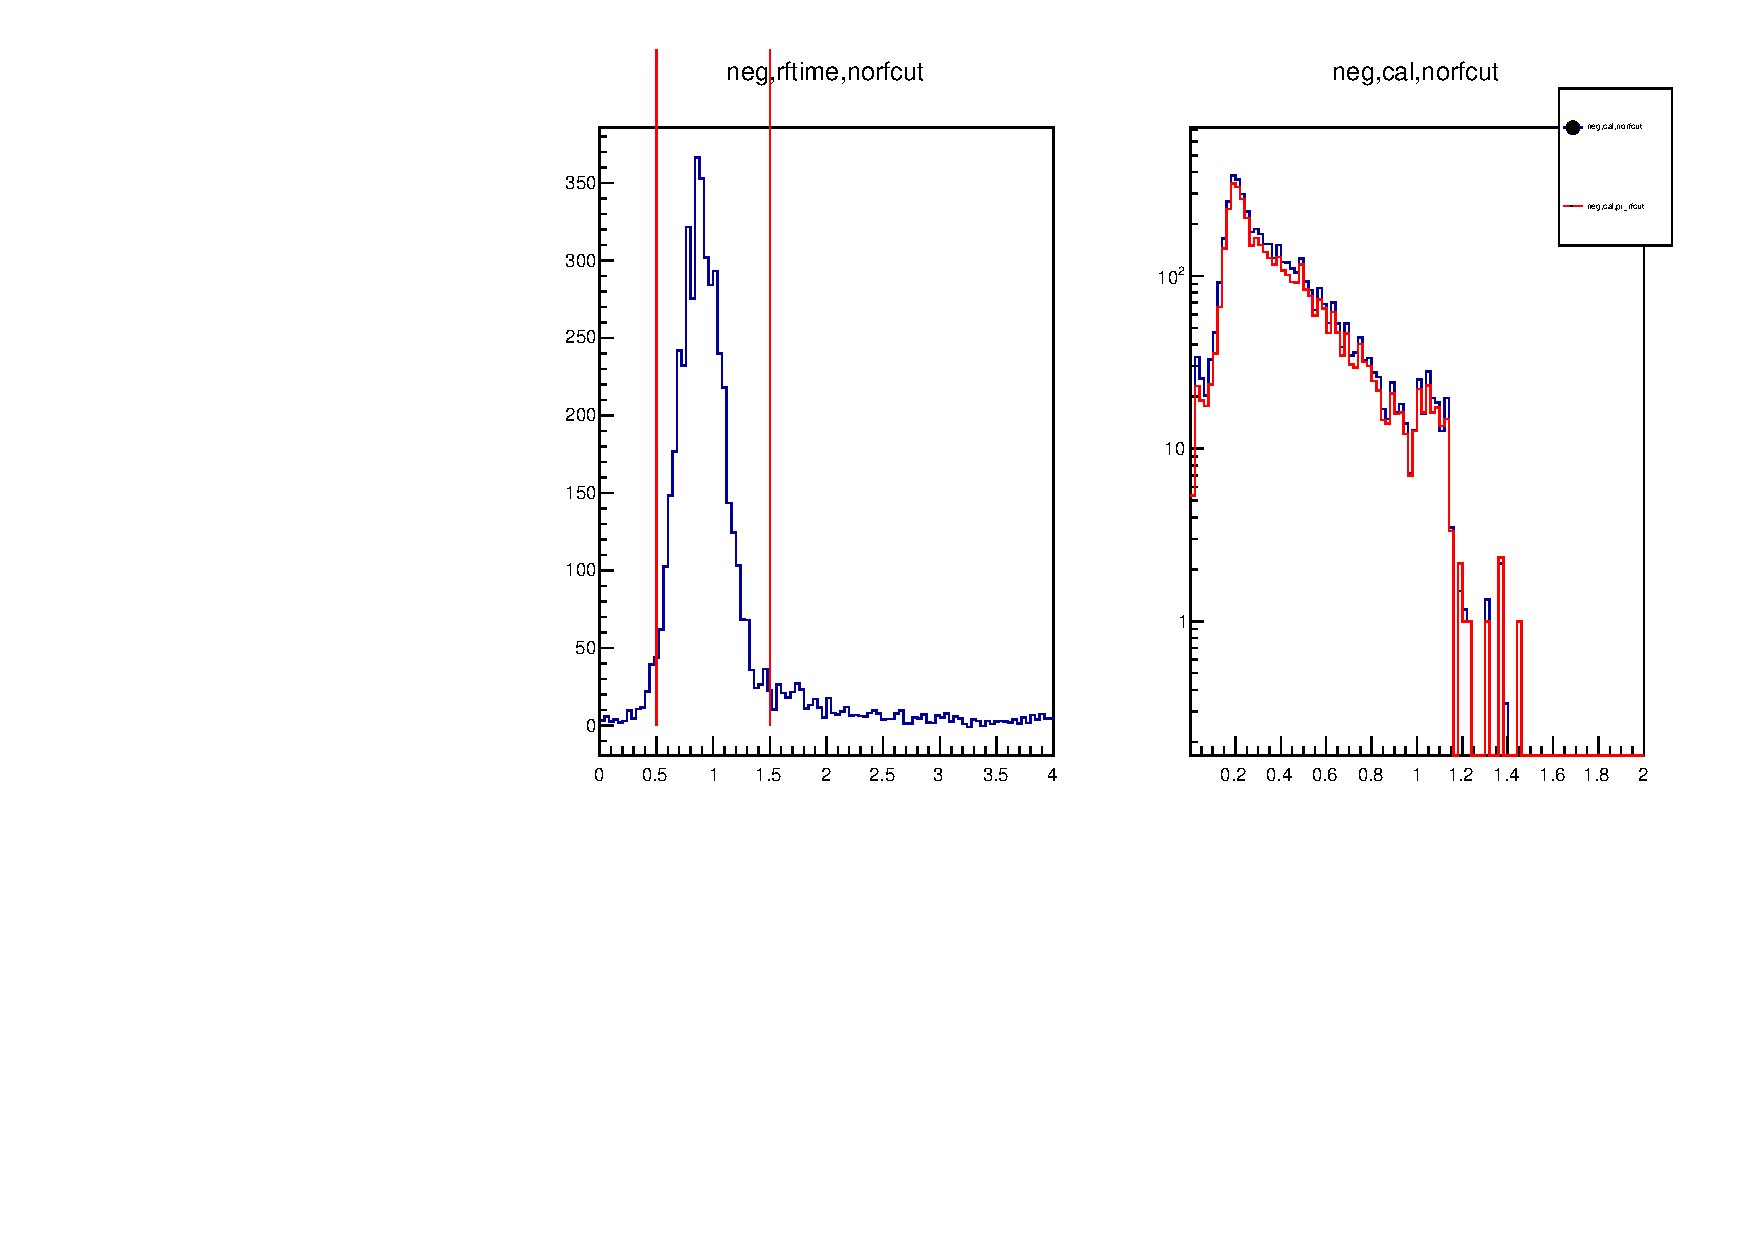
\includegraphics[width = 0.8\textwidth]{results/pid/SHMS_cal_DE_6524.pdf}
  \\
  neg run 6524,in run group 360, momentum 4.736
\end{frame}
\begin{frame}{SHMS efficiency with cut}
  \begin{columns}
    \begin{column}[T]{0.5\textwidth}
  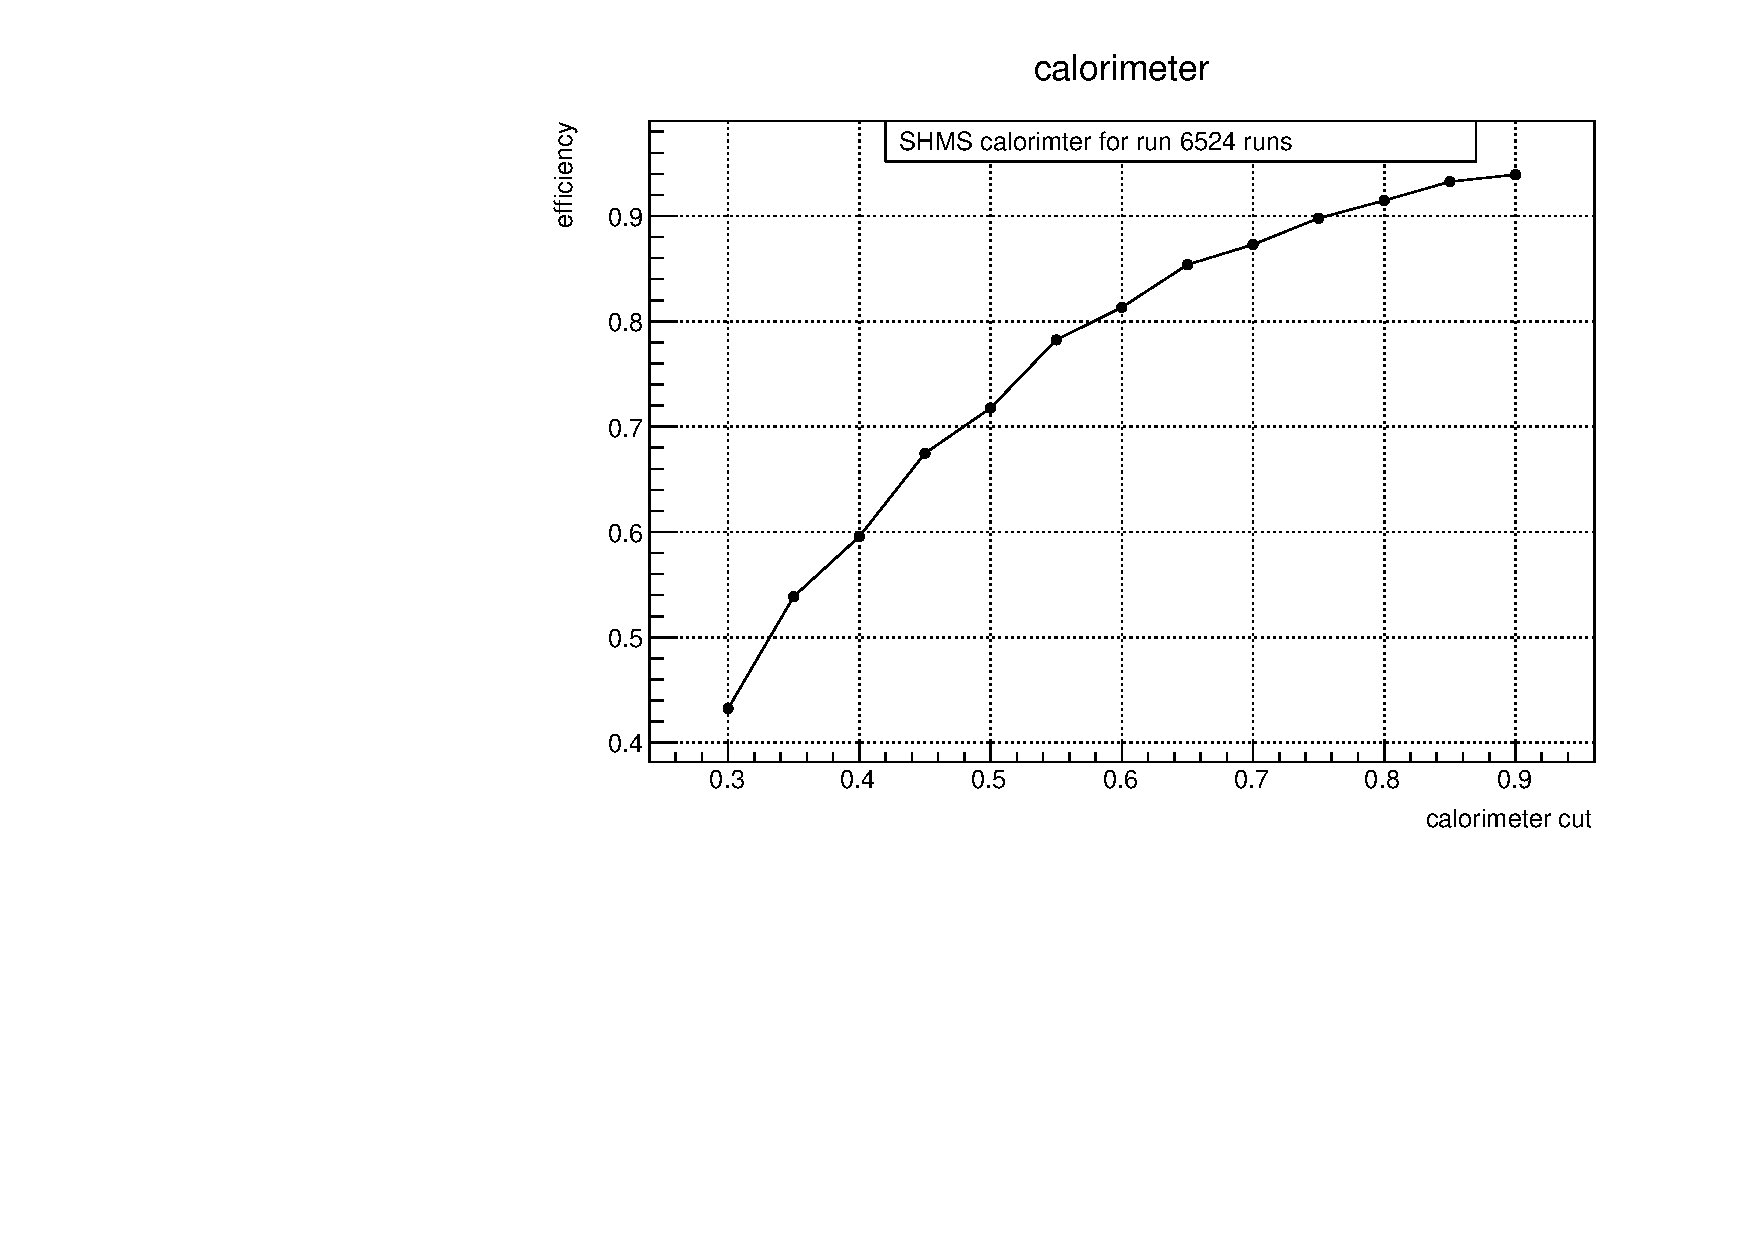
\includegraphics[width = 0.8\textwidth]{results/pid/SHMS_cal_6524.pdf}
\end{column}
\begin{column}[T]{0.5\textwidth}
  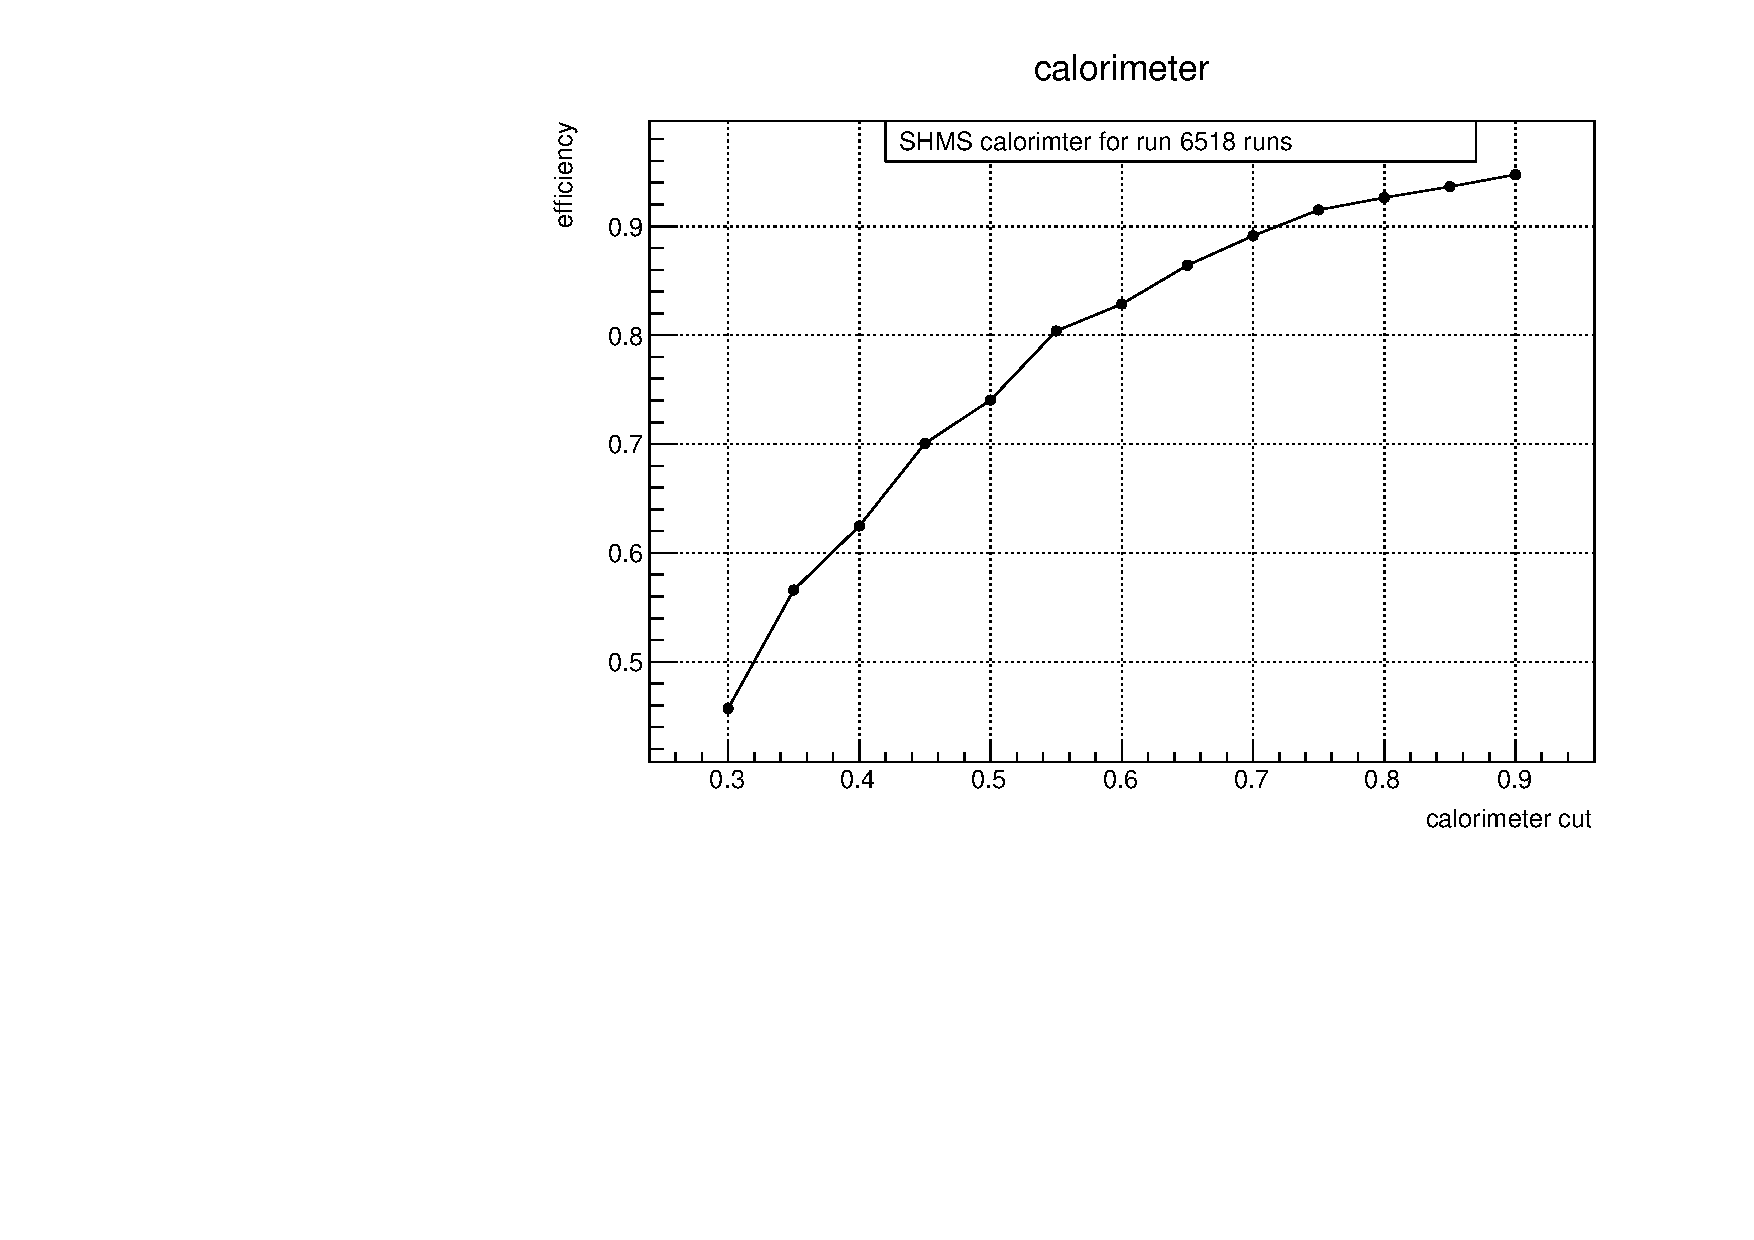
\includegraphics[width = 0.8\textwidth]{results/pid/SHMS_cal_6518.pdf}
\end{column}
\end{columns}
  \\
  left is neg run 6524,right is pos run 6518, in run group 360, momentum 4.736
 
\end{frame}
\begin{frame}{SHMS cal efficiency verse momentum}
  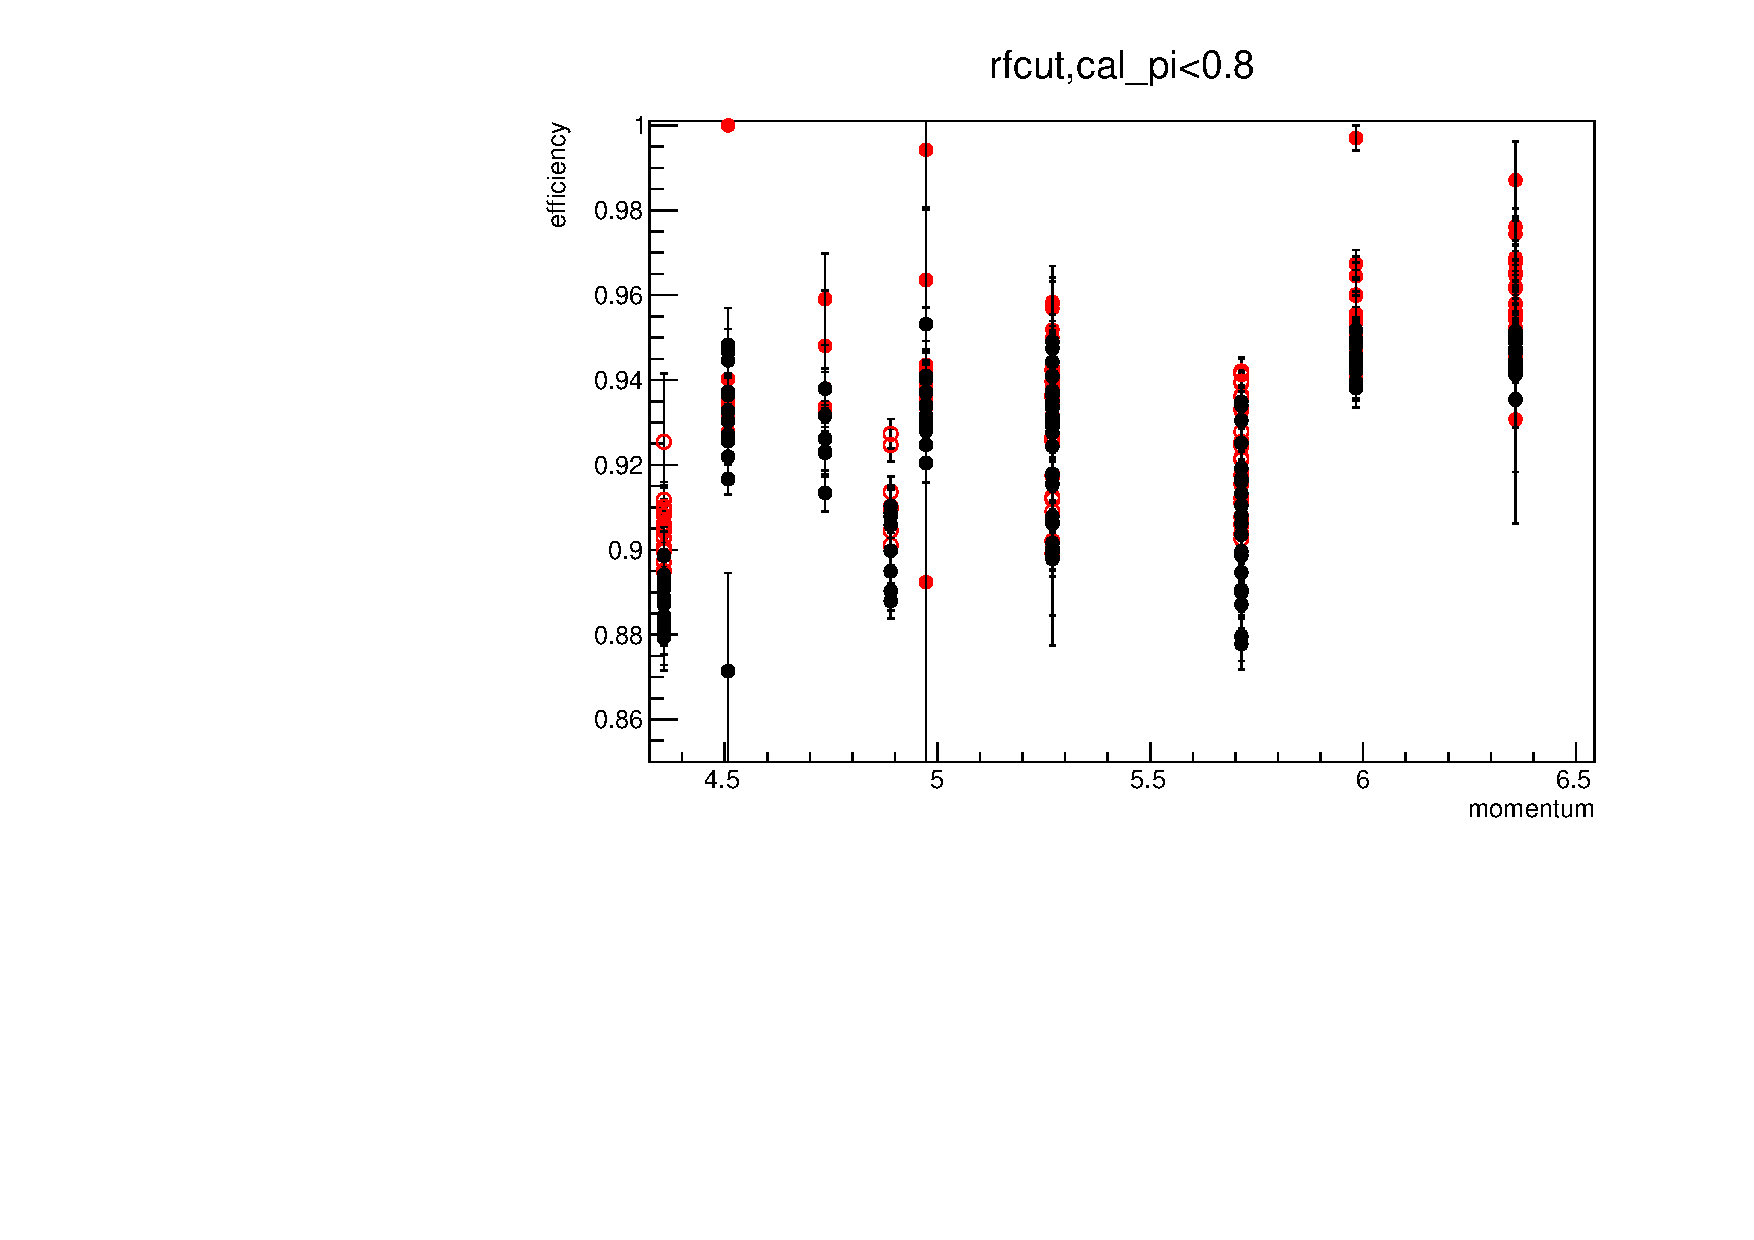
\includegraphics[width = 0.8\textwidth]{results/pid/SHMS_cal_DE_momentum.pdf}
\end{frame}
\begin{frame}{SHMS cal efficiency verse RunNumber}
  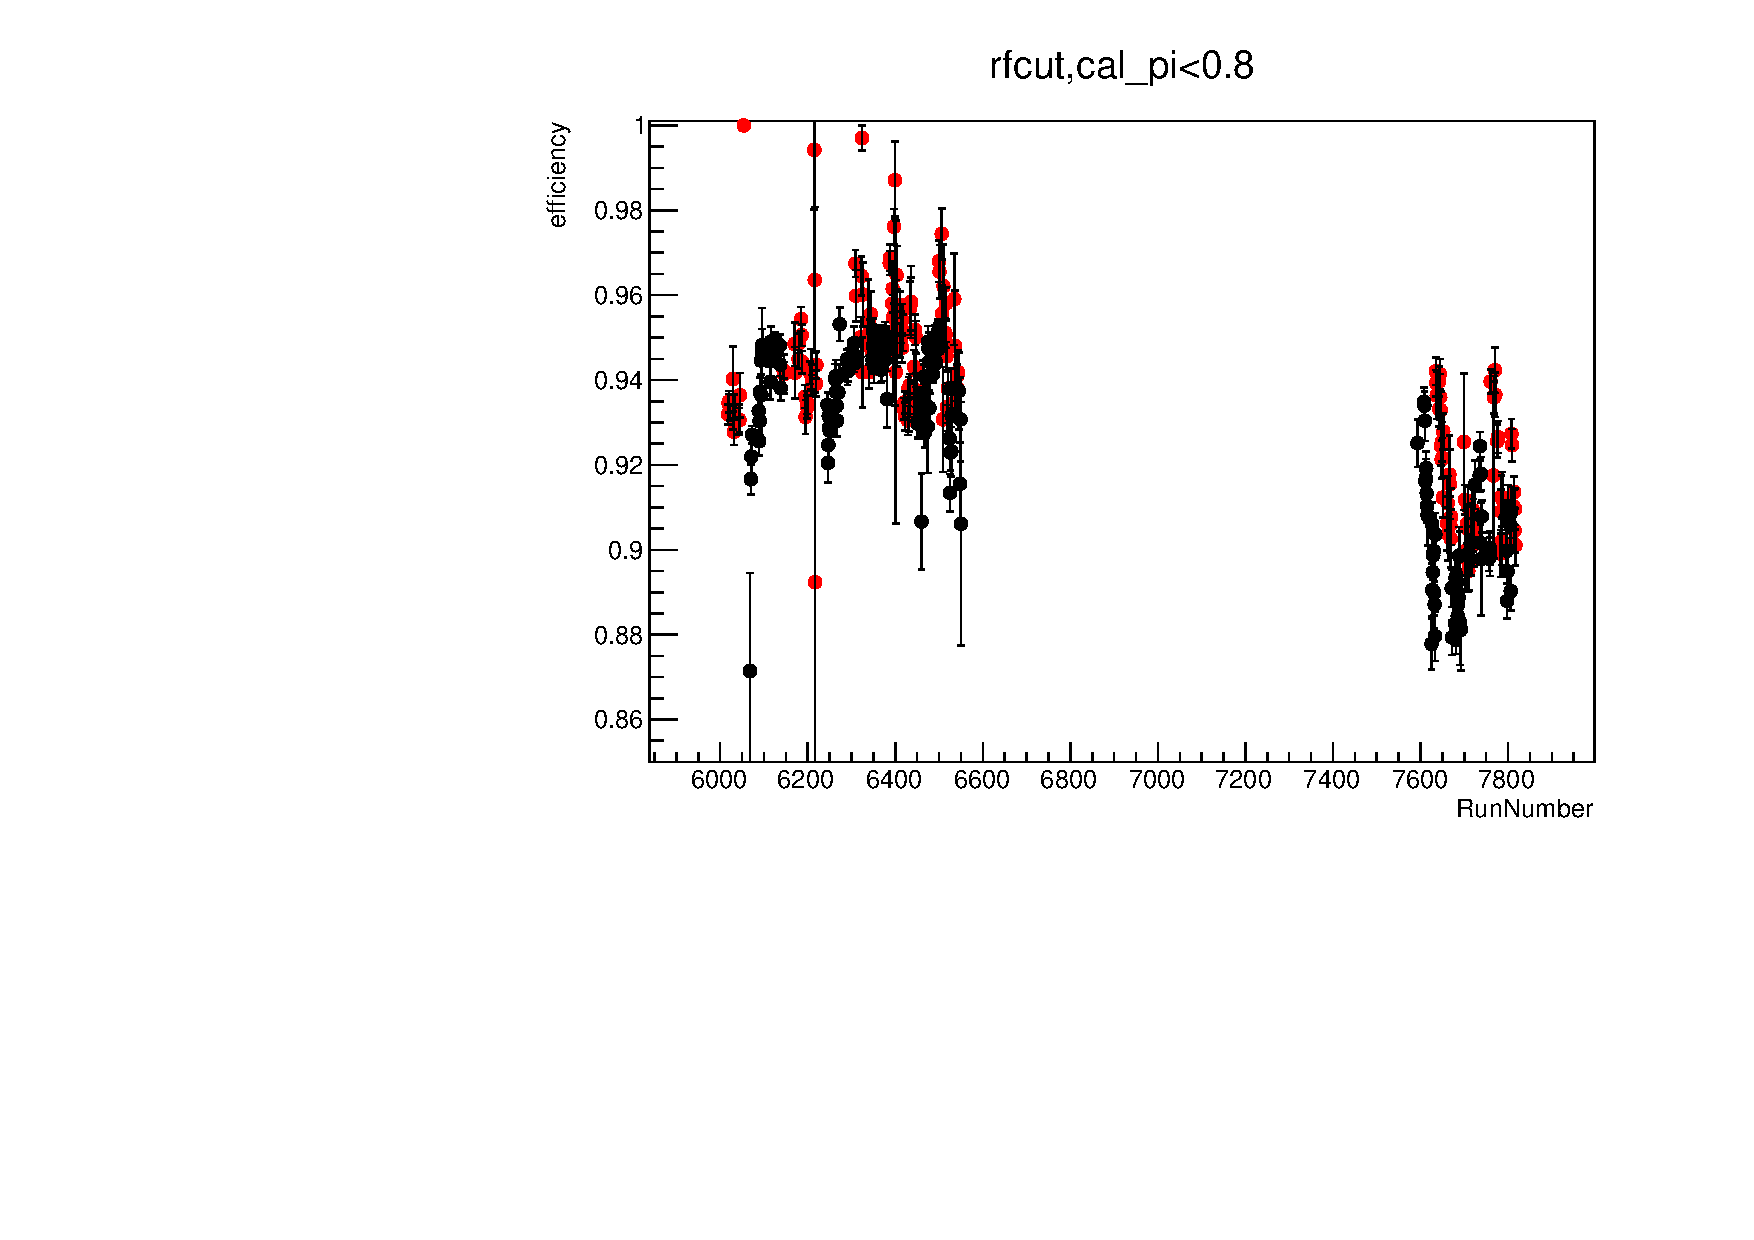
\includegraphics[width = 0.8\textwidth]{results/pid/SHMS_cal_DE_RunNumber.pdf}
\end{frame}
\begin{frame}{SHMS cal efficiency verse RunNumber}
  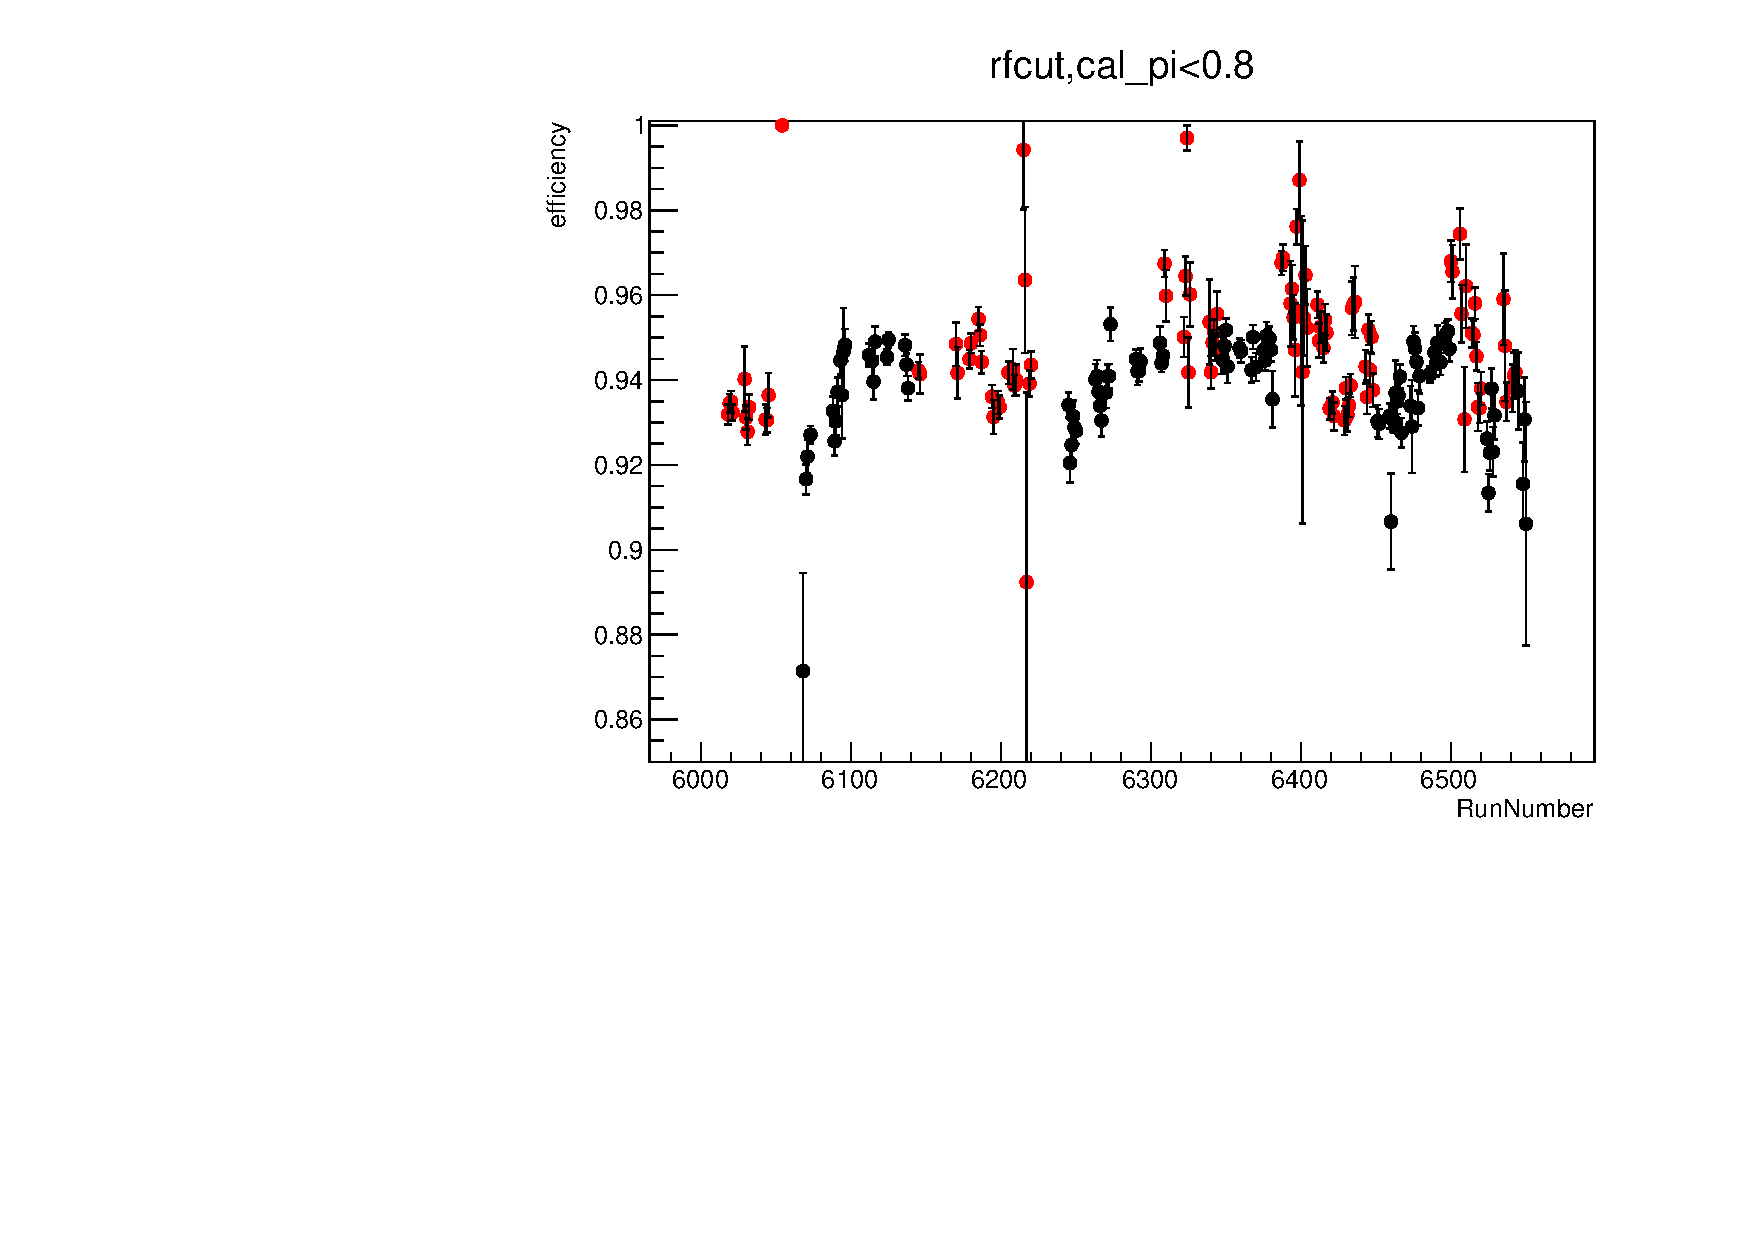
\includegraphics[width = 0.8\textwidth]{results/pid/SHMS_cal_DE_RunNumber_fall.pdf}
\end{frame}
\begin{frame}{SHMS cal efficiency verse RunNumber}
  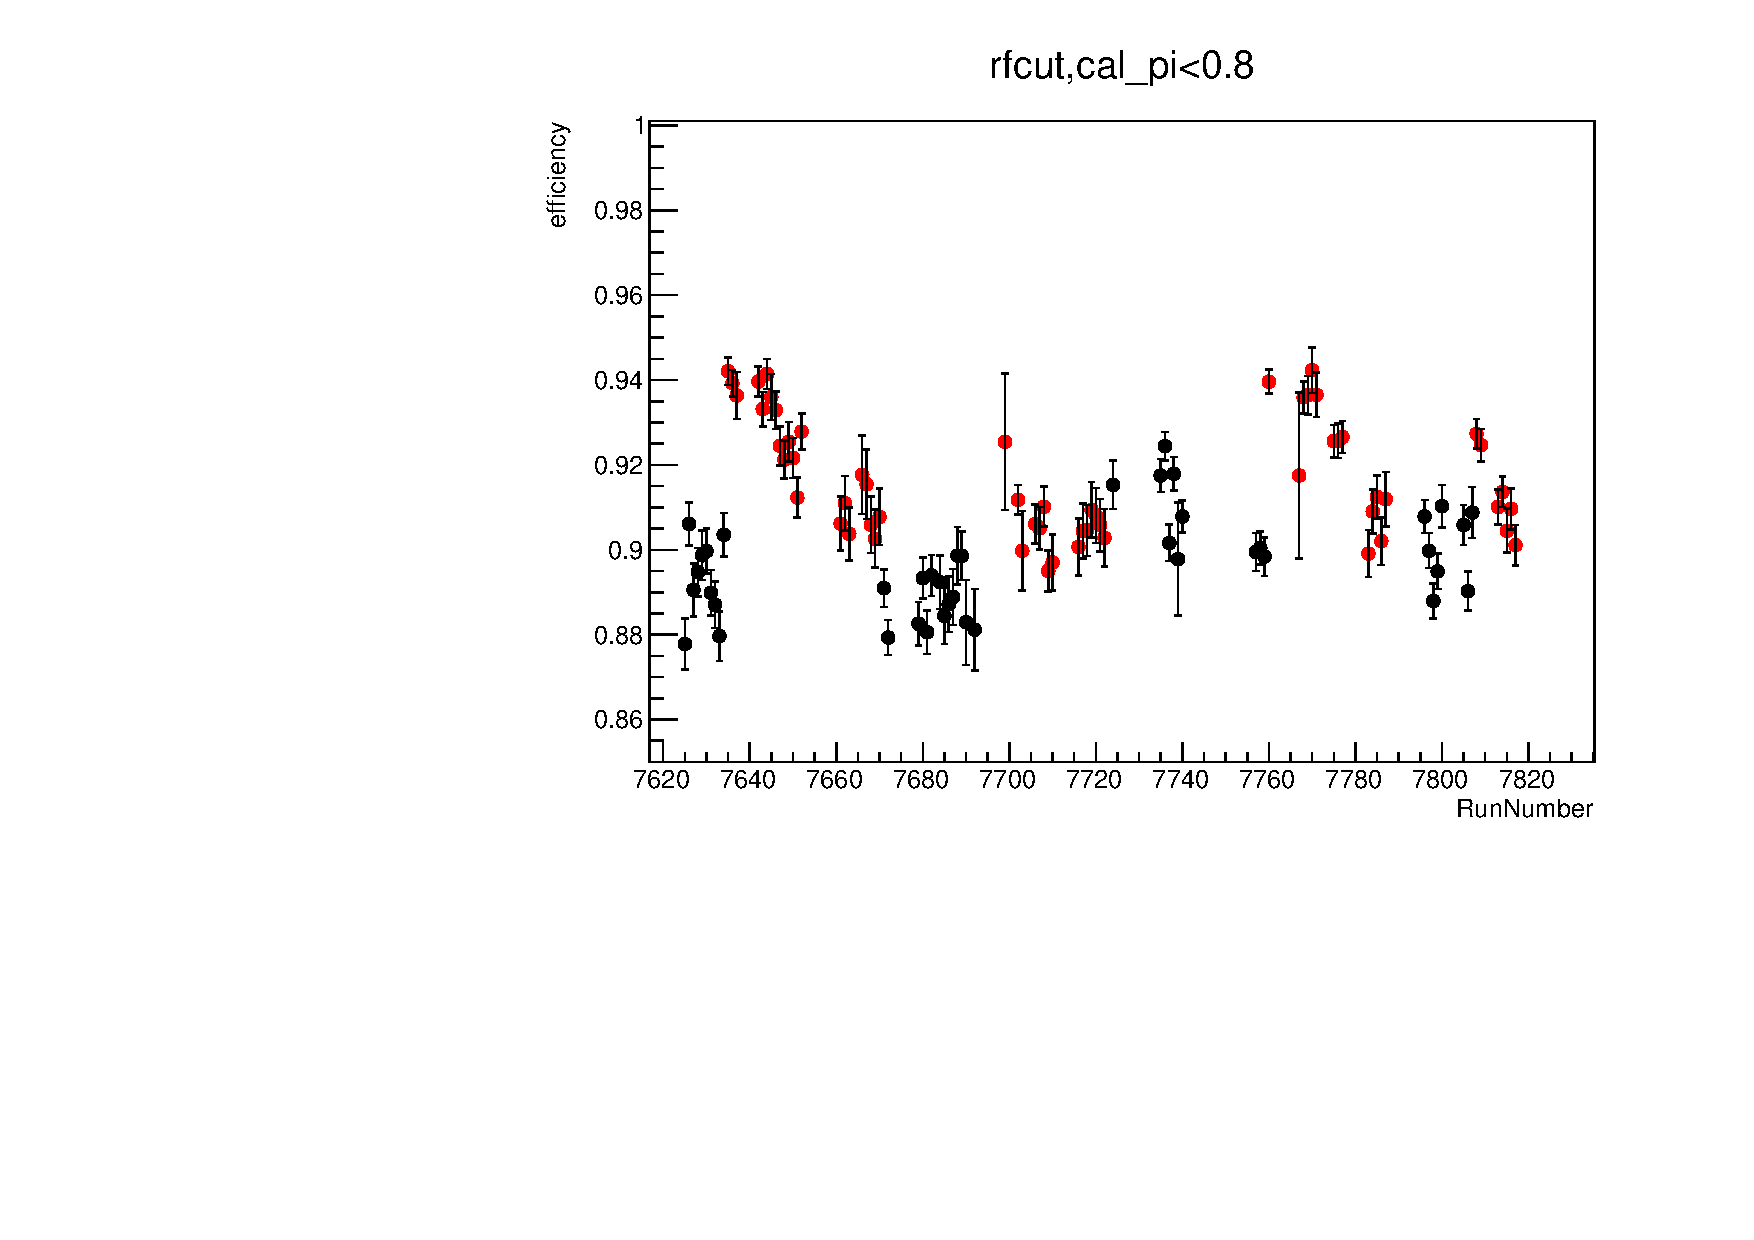
\includegraphics[width = 0.8\textwidth]{results/pid/SHMS_cal_DE_RunNumber_spring.pdf}
\end{frame}
\begin{frame}{SHMS cal efficiency verse RunGroup}
  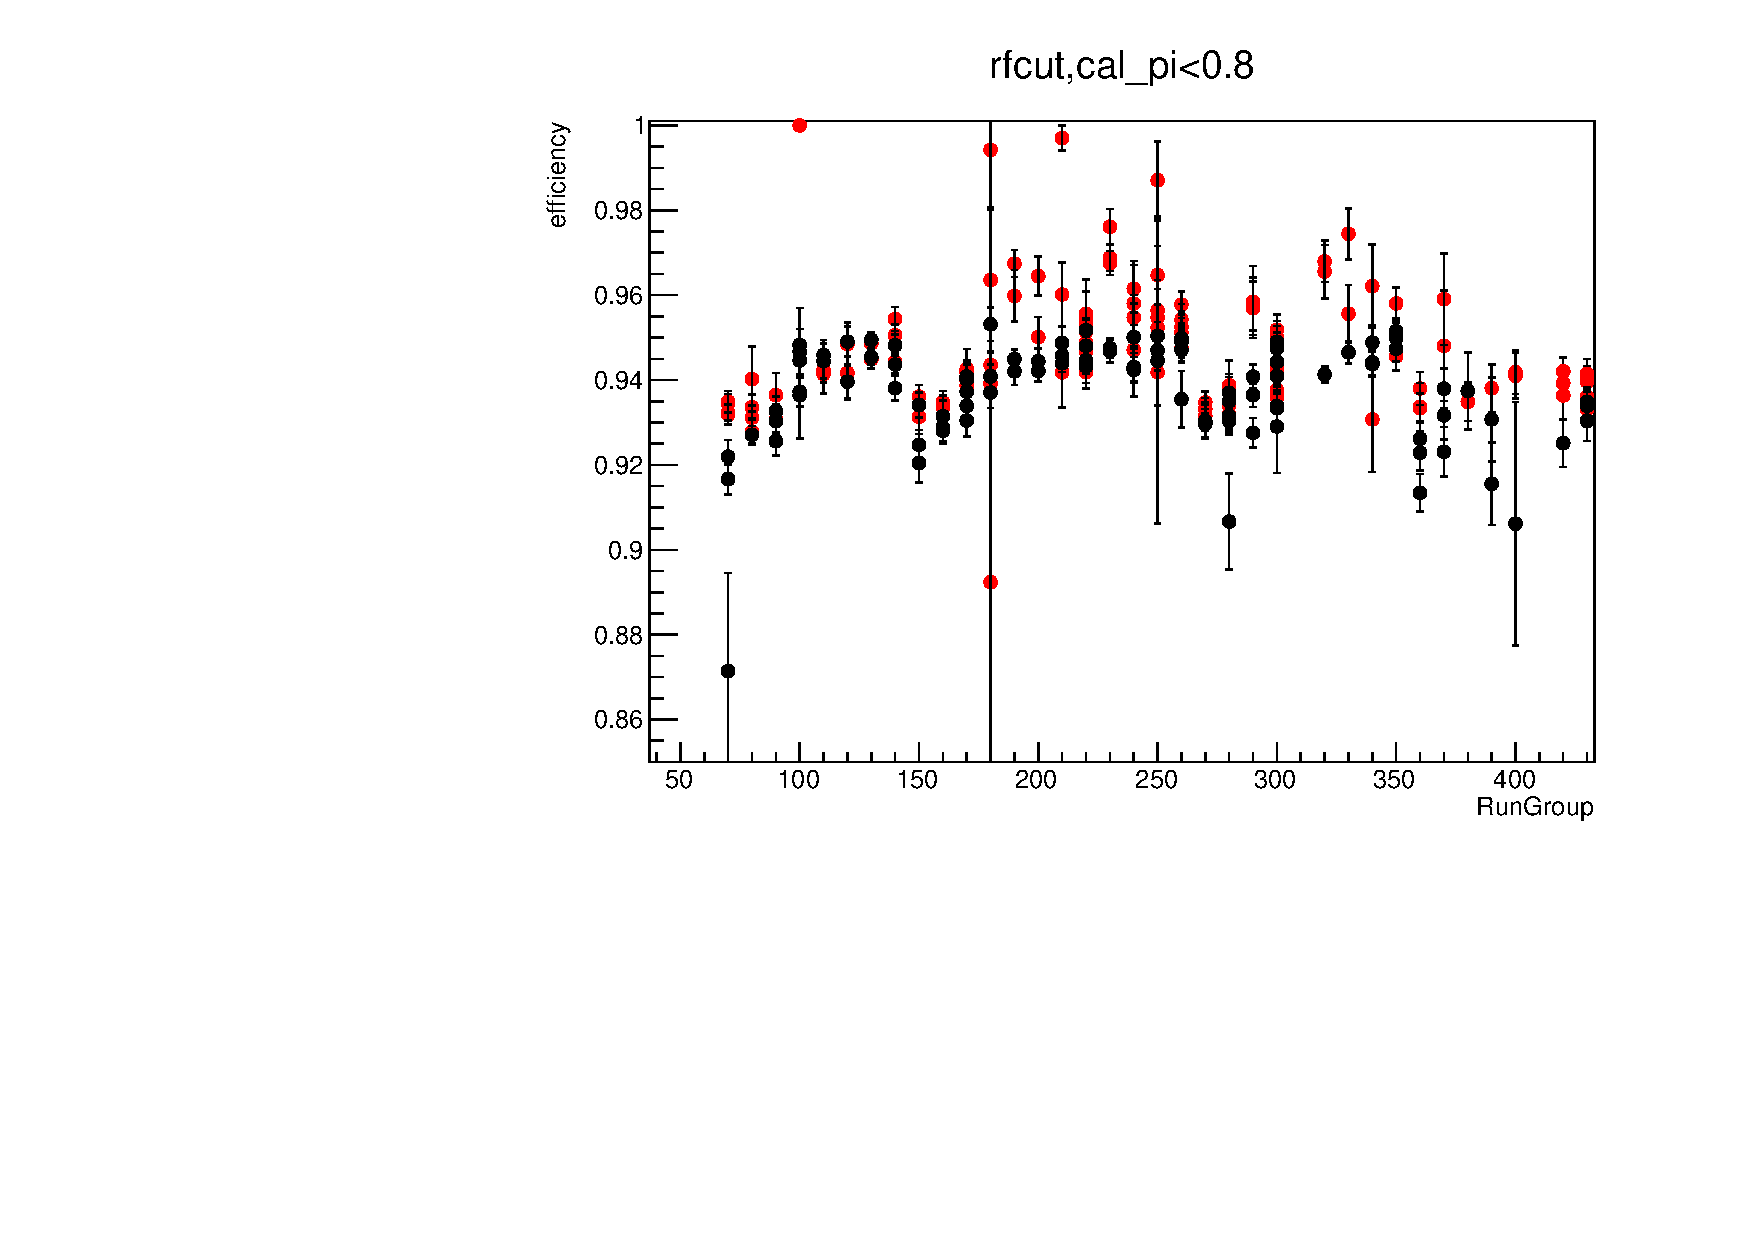
\includegraphics[width = 0.8\textwidth]{results/pid/SHMS_cal_DE_RunGroup.pdf}
\end{frame}
\begin{frame}{SHMS efficiency with cut}
  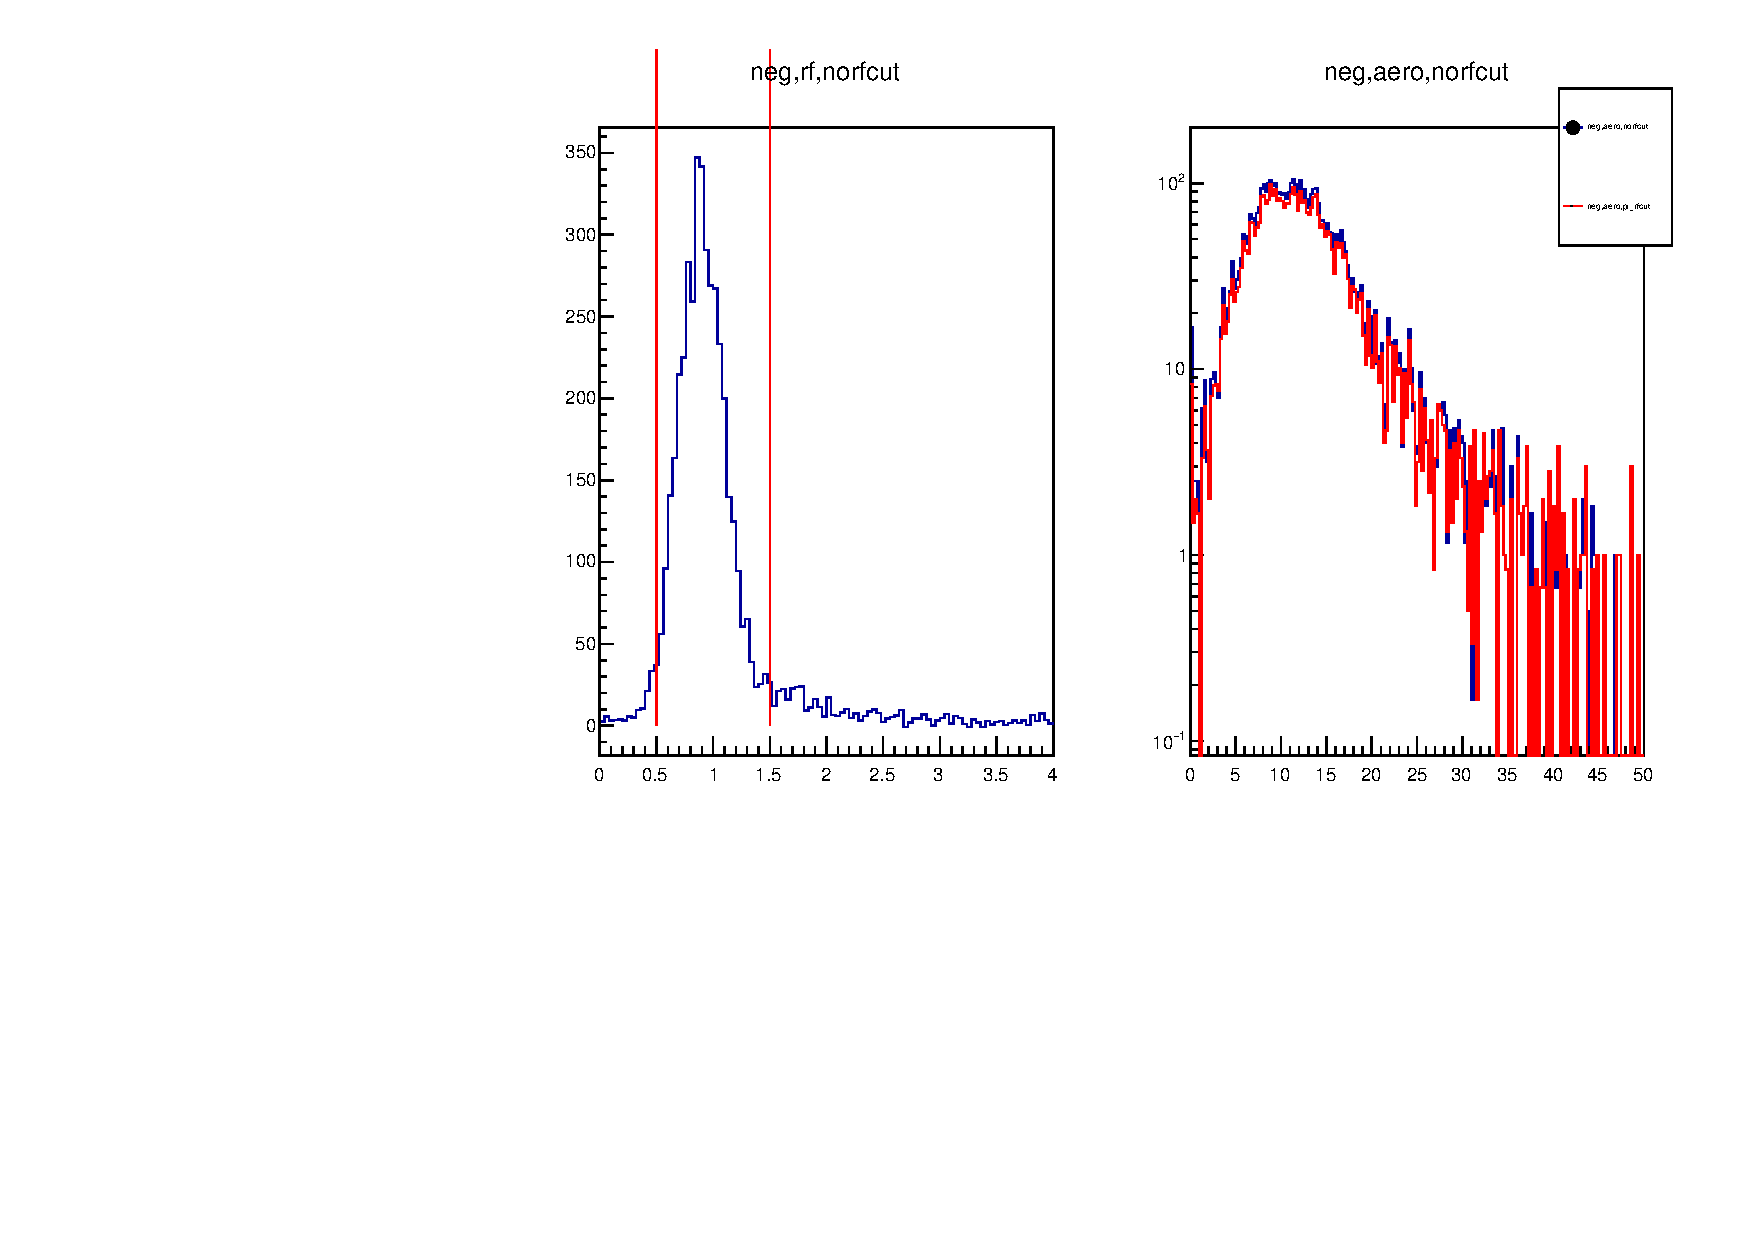
\includegraphics[width = 0.8\textwidth]{results/pid/SHMS_aero_DE_6524.pdf}
  \\
   neg run 6524,in run group 360, momentum 4.736
 
\end{frame}
\begin{frame}{efficiency with cut}
  \begin{columns}
    \begin{column}[T]{0.5\textwidth}
  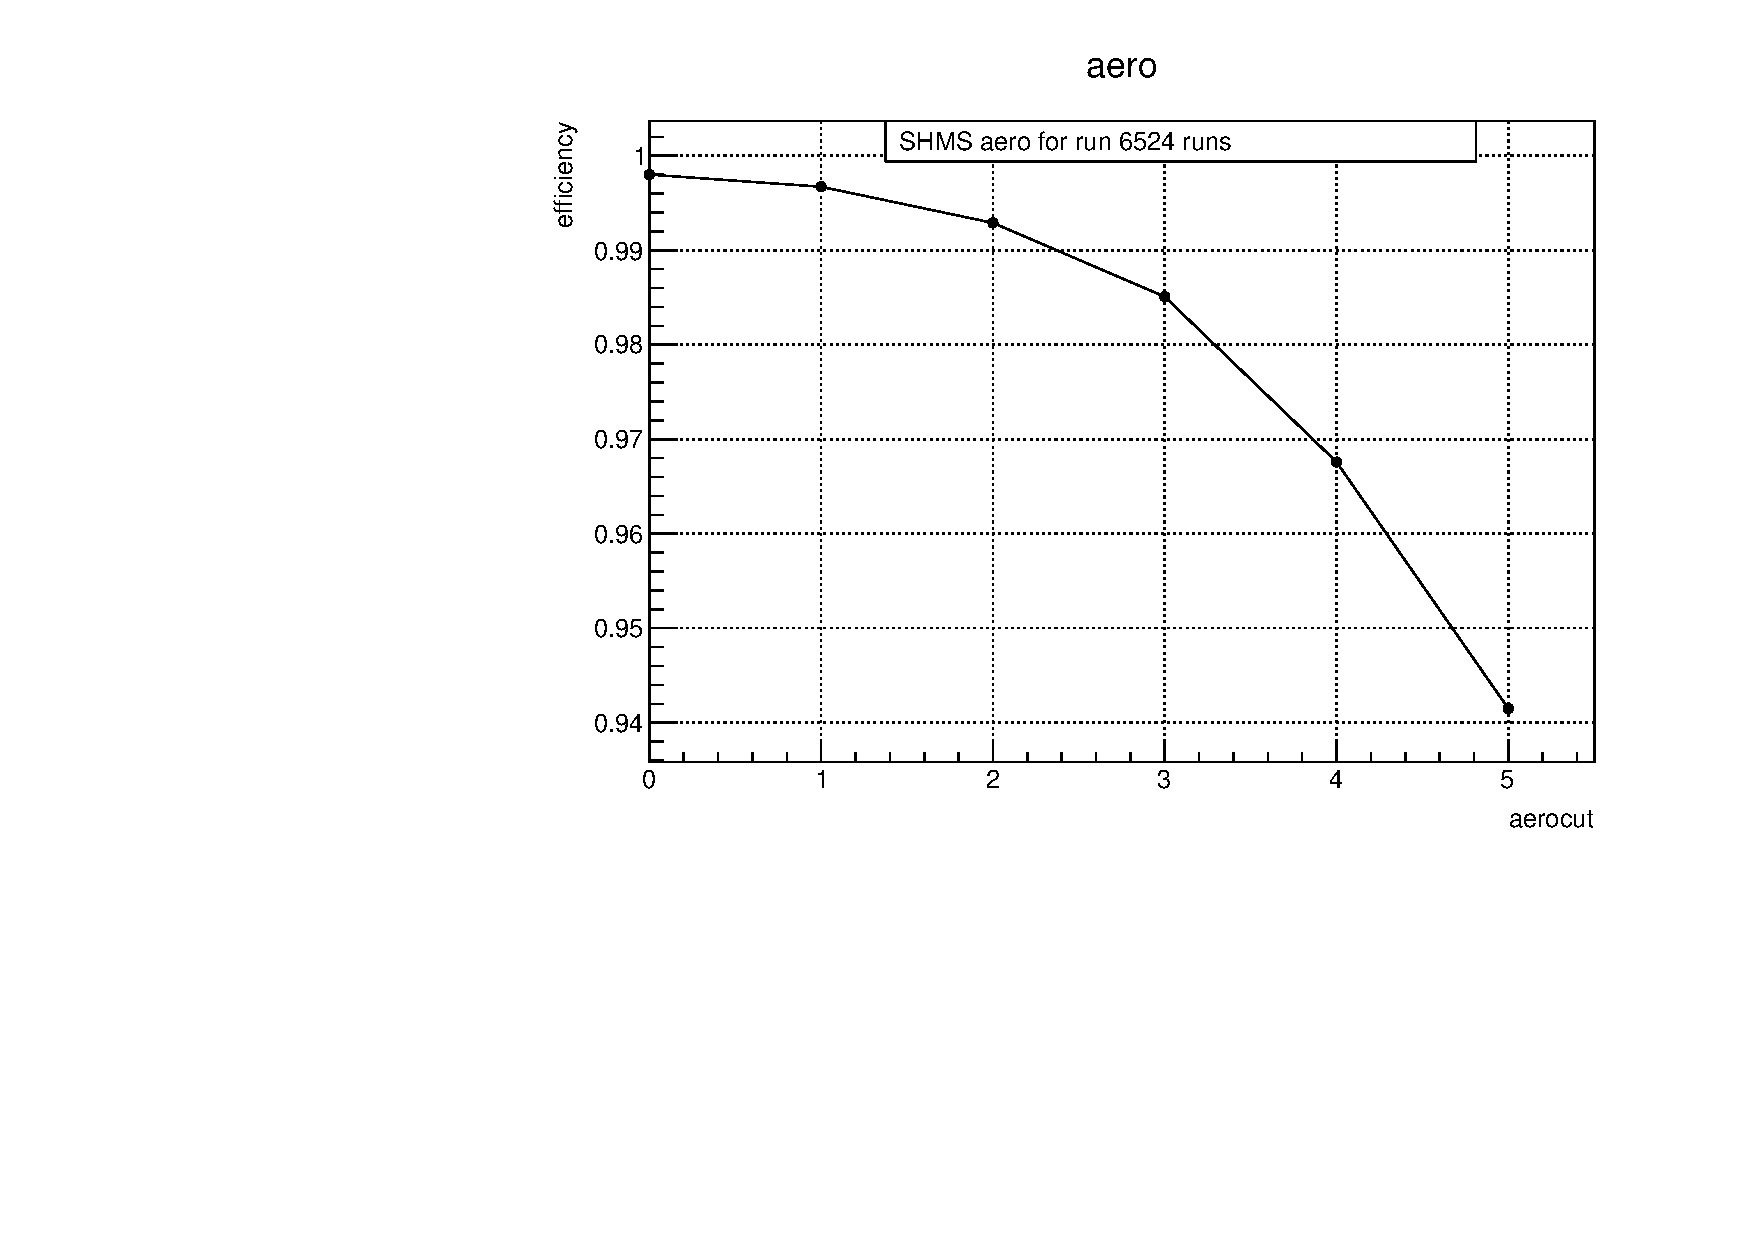
\includegraphics[width = 0.8\textwidth]{results/pid/SHMS_aero_6524.pdf}
\end{column}
\begin{column}[T]{0.5\textwidth}
  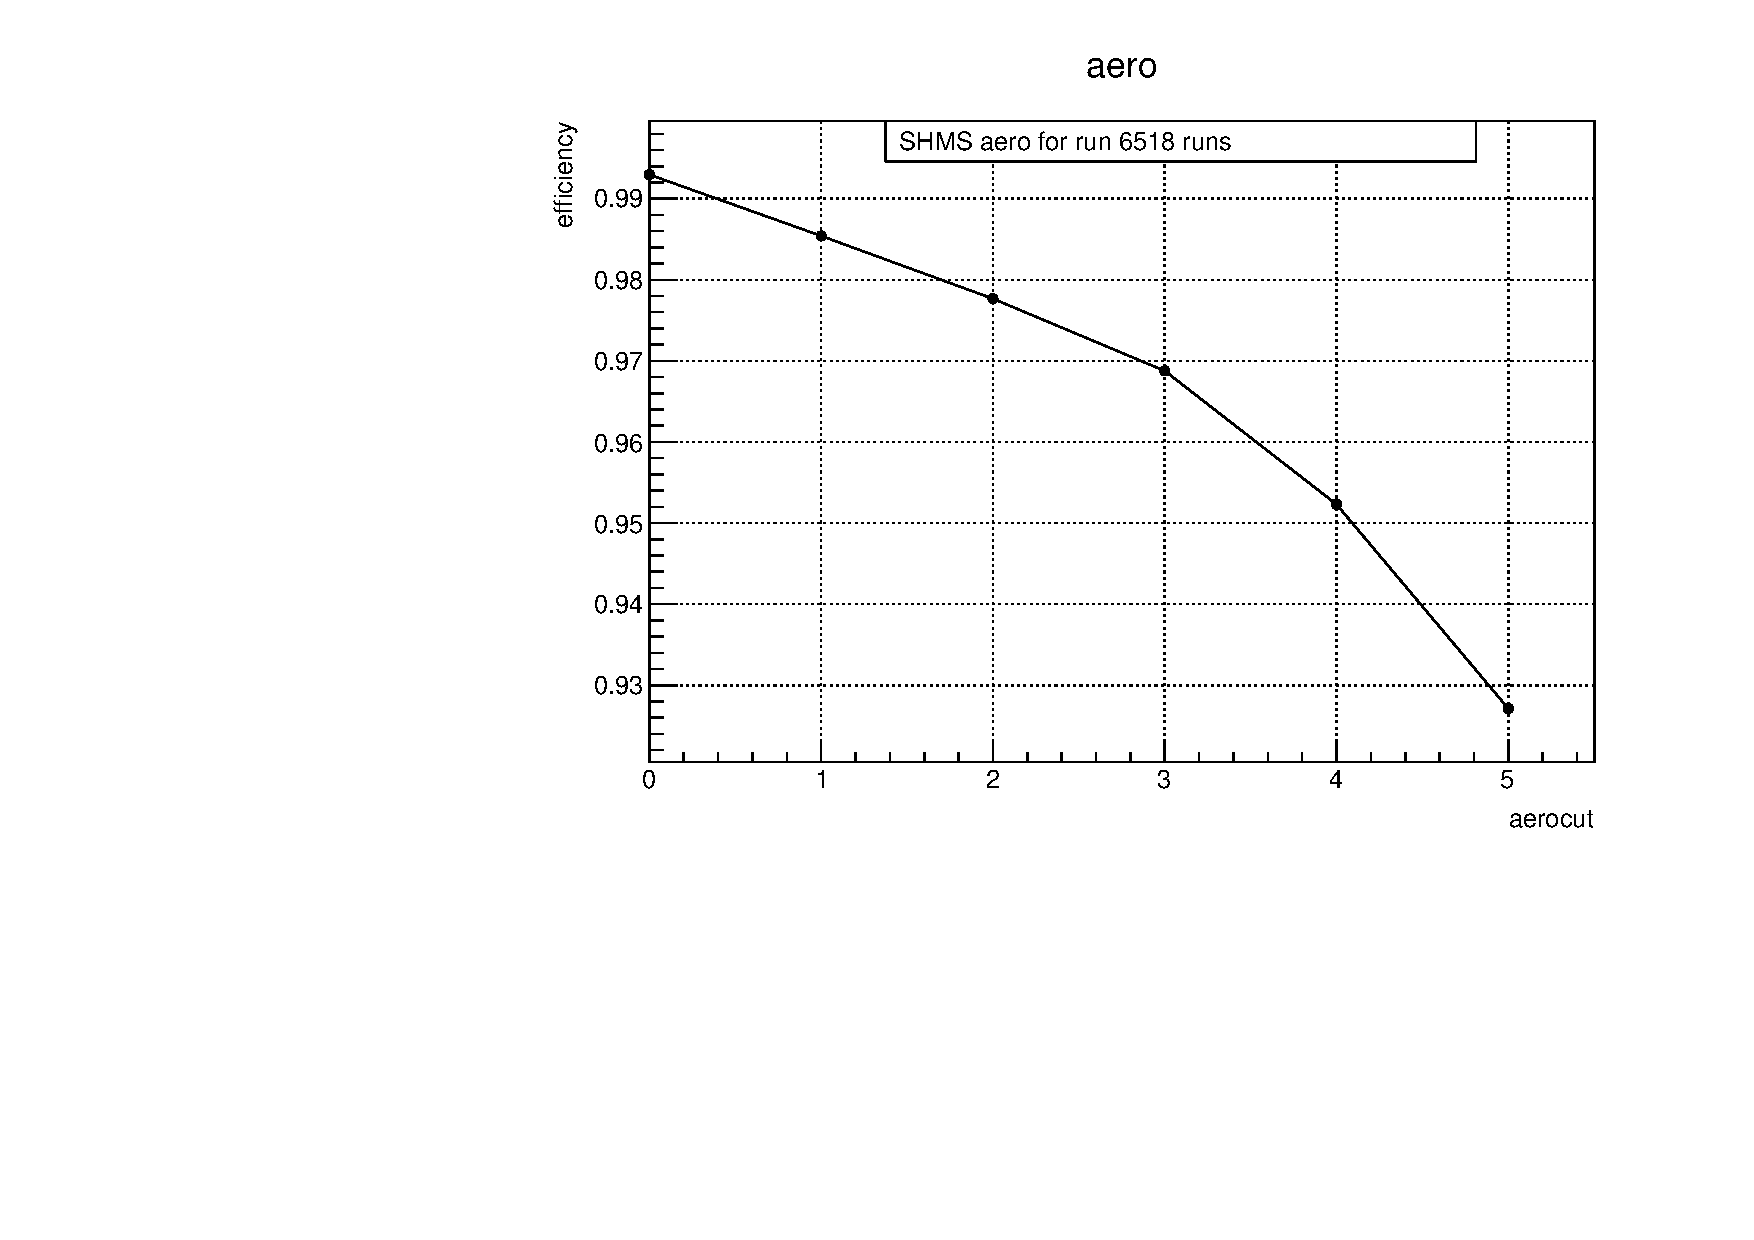
\includegraphics[width = 0.8\textwidth]{results/pid/SHMS_aero_6518.pdf}
\end{column}
\end{columns}
  \\
   neg run 6524,in run group 360, momentum 4.736
 
\end{frame}

\begin{frame}{SHMS aero efficiency verse momentum}
  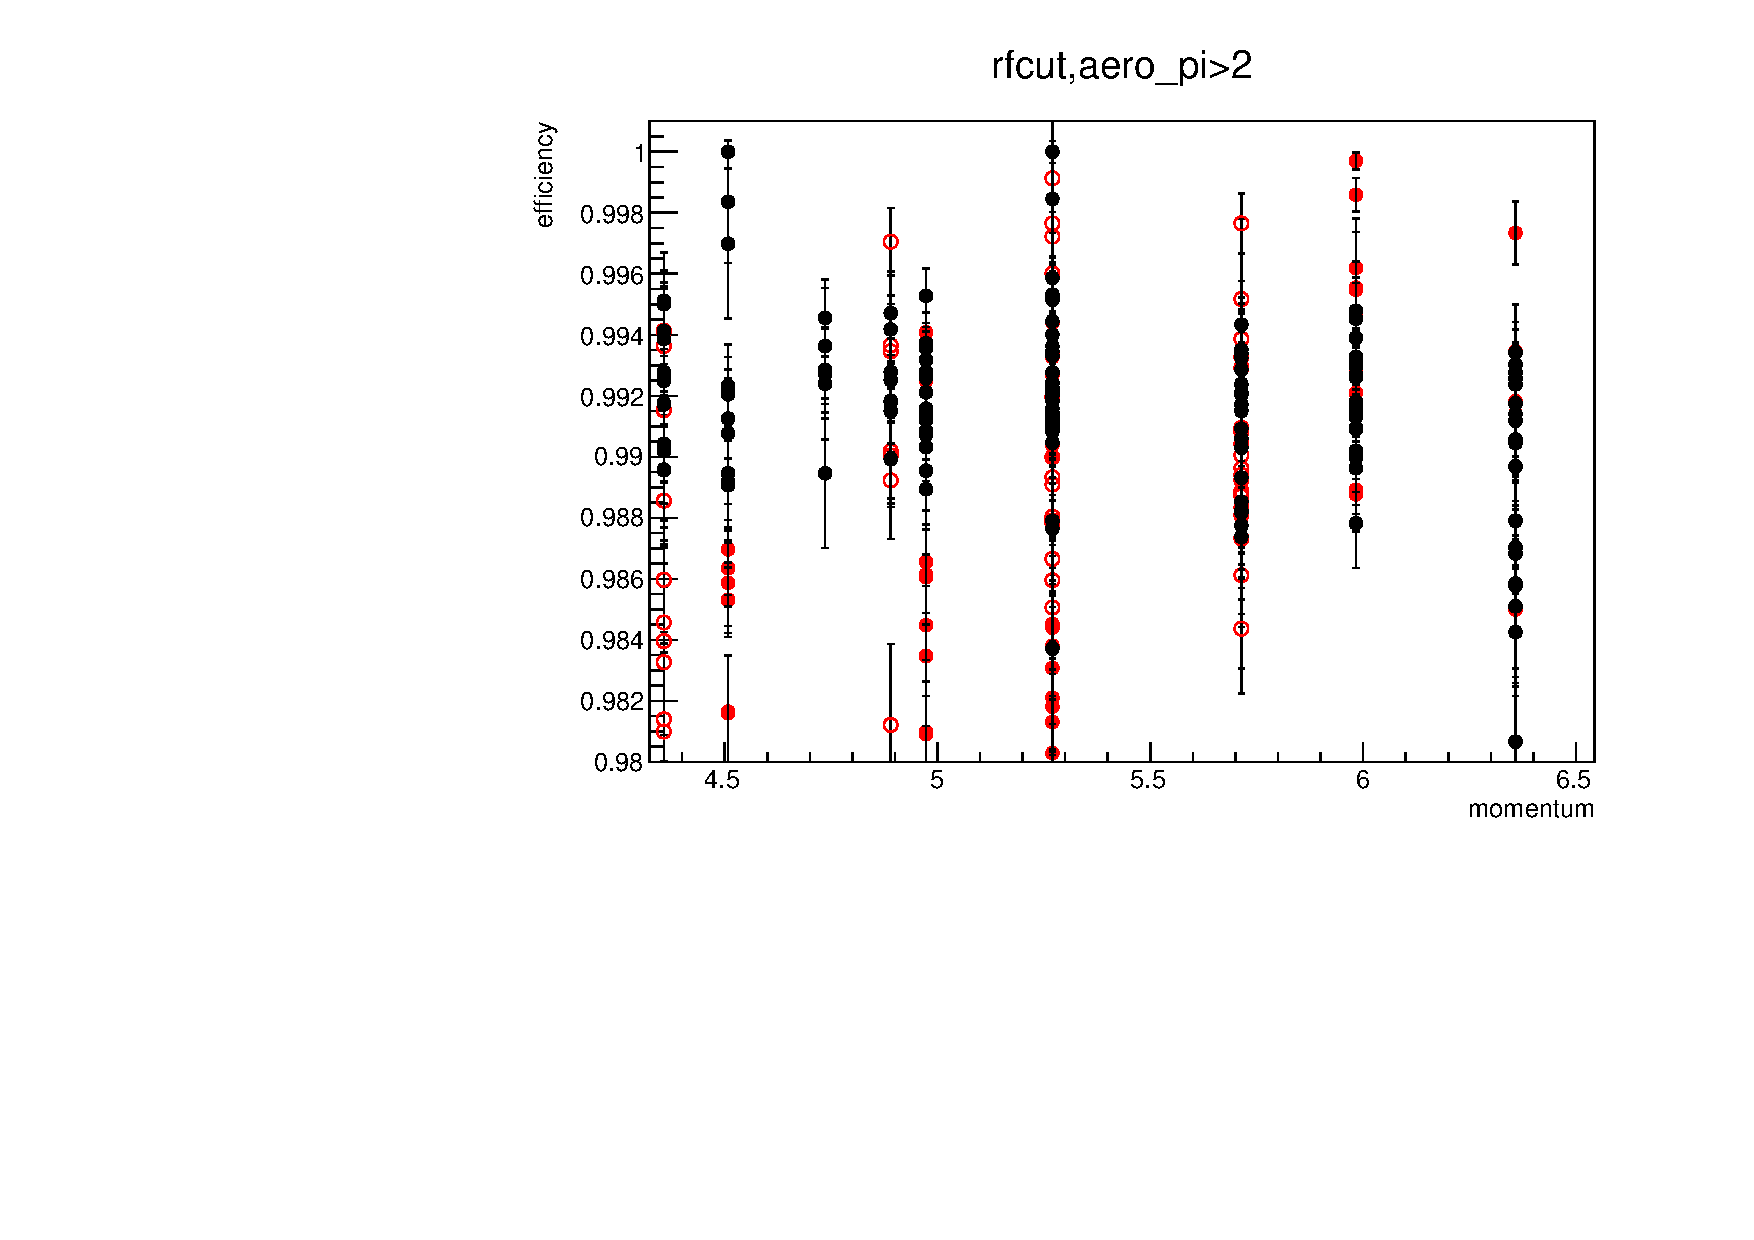
\includegraphics[width = 0.8\textwidth]{results/pid/SHMS_aero_DE_momentum.pdf}
\end{frame}
\begin{frame}{SHMS aero efficiency verse RunNumber}
  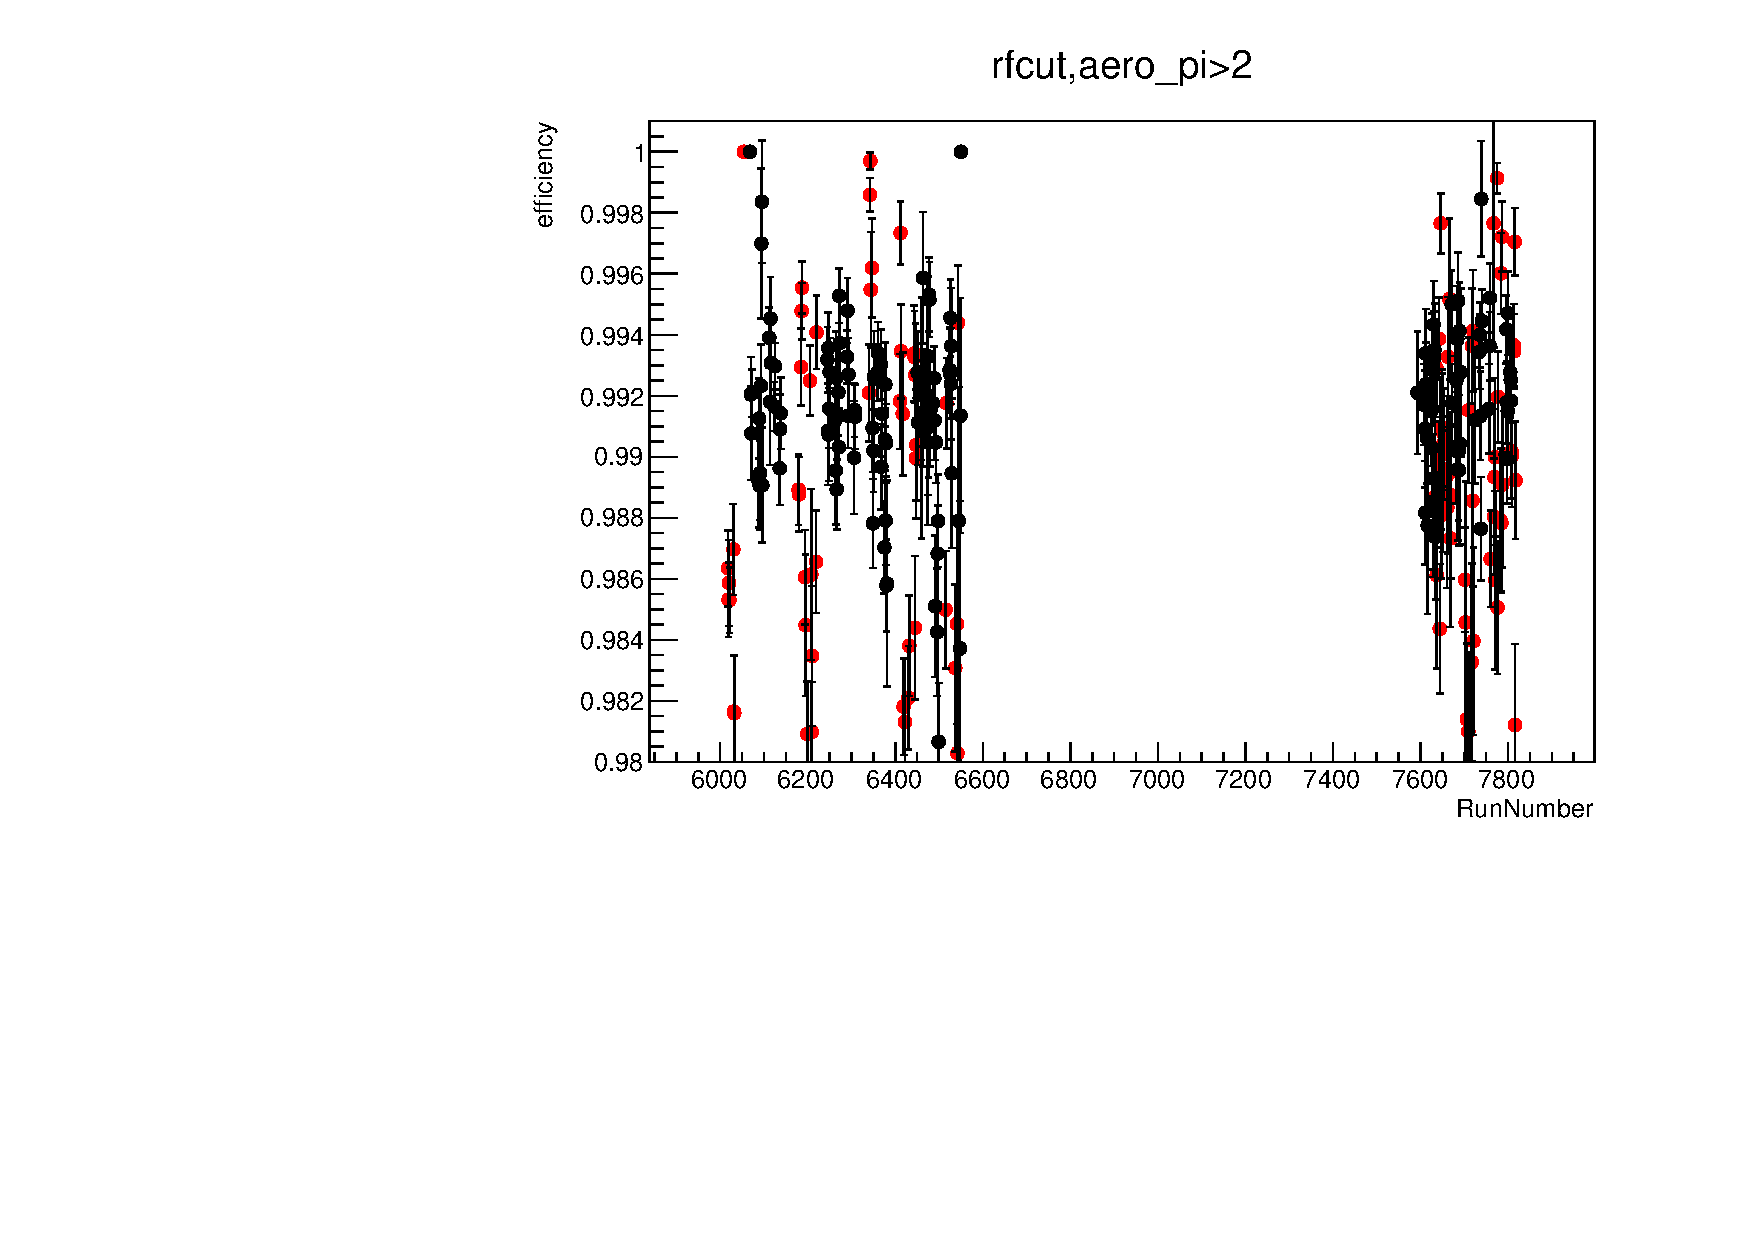
\includegraphics[width = 0.8\textwidth]{results/pid/SHMS_aero_DE_RunNumber.pdf}
\end{frame}
\begin{frame}{SHMS aero efficiency verse RunNumber}
  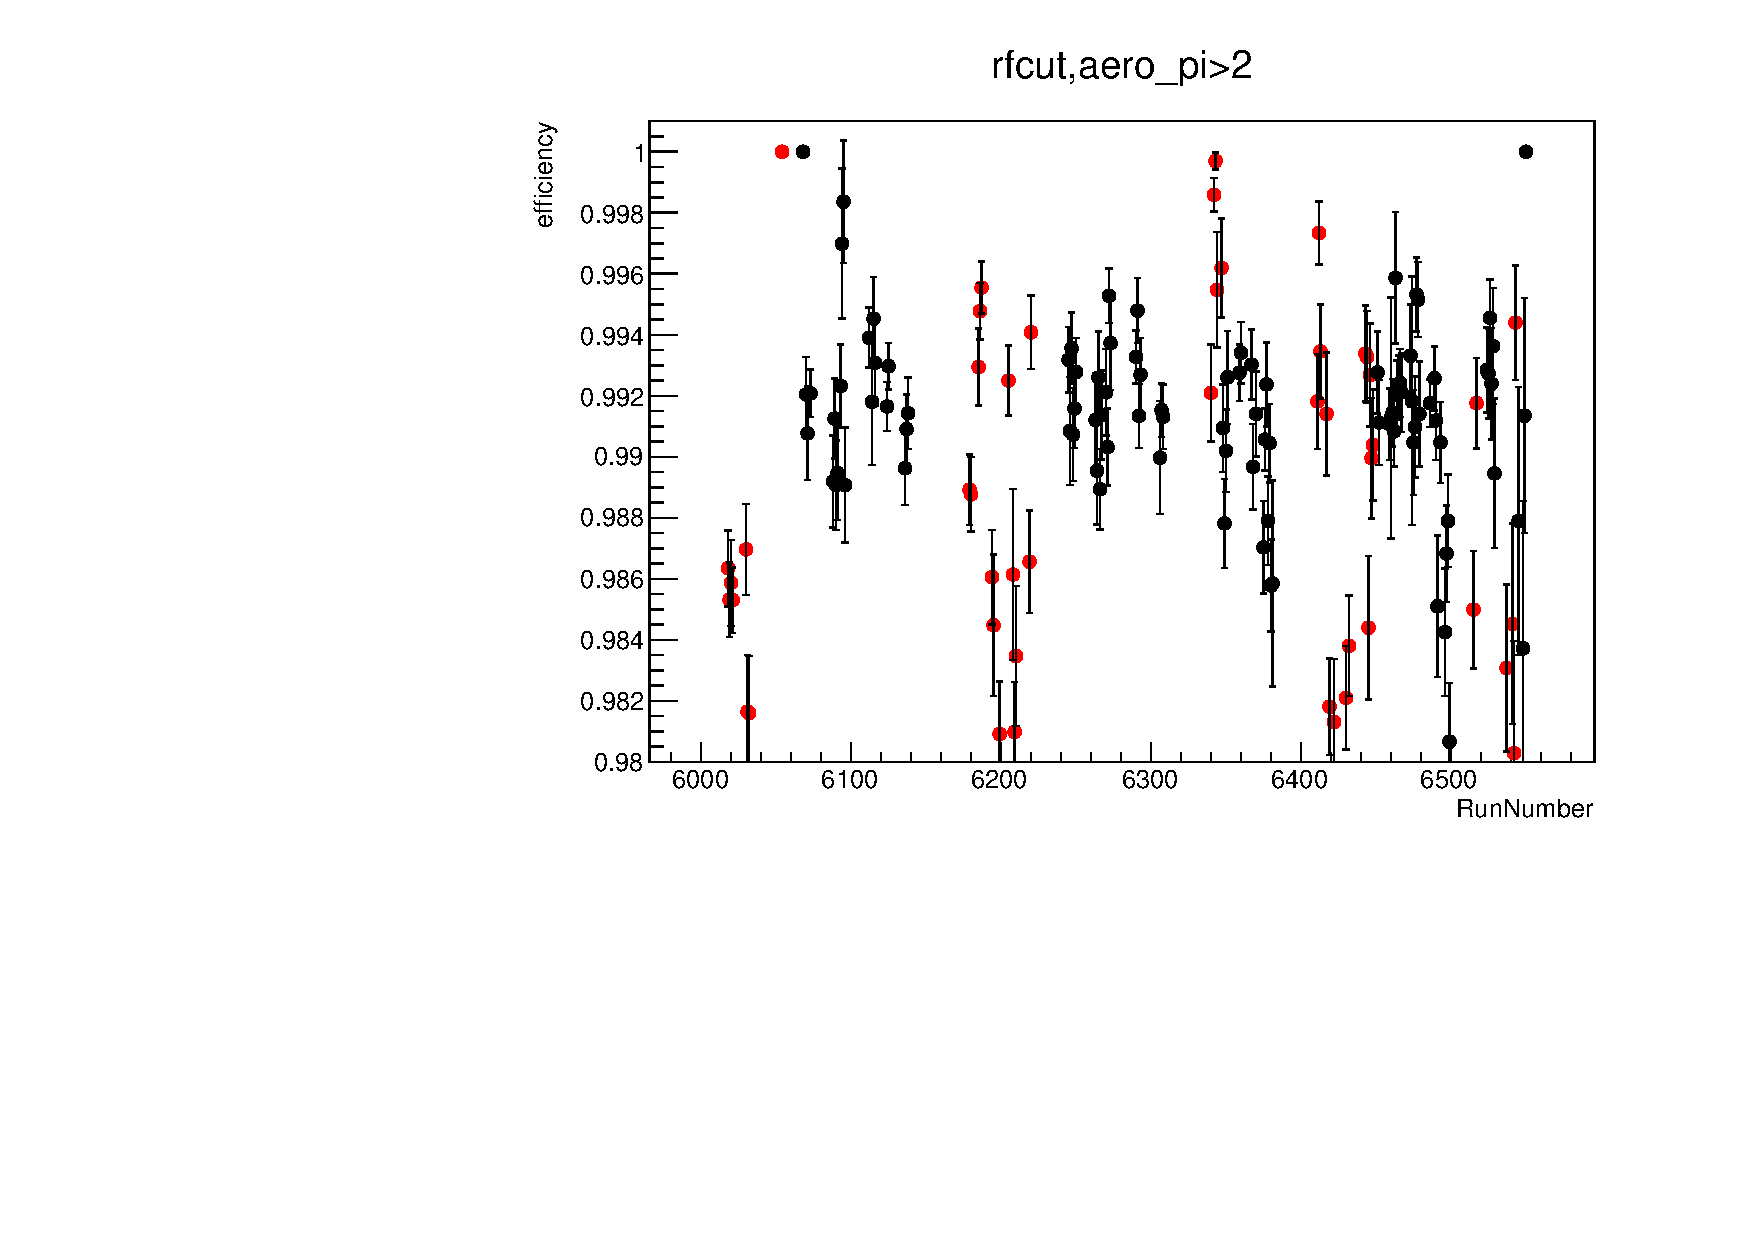
\includegraphics[width = 0.8\textwidth]{results/pid/SHMS_aero_DE_RunNumber_fall.pdf}
\end{frame}
\begin{frame}{SHMS aero efficiency verse RunNumber}
  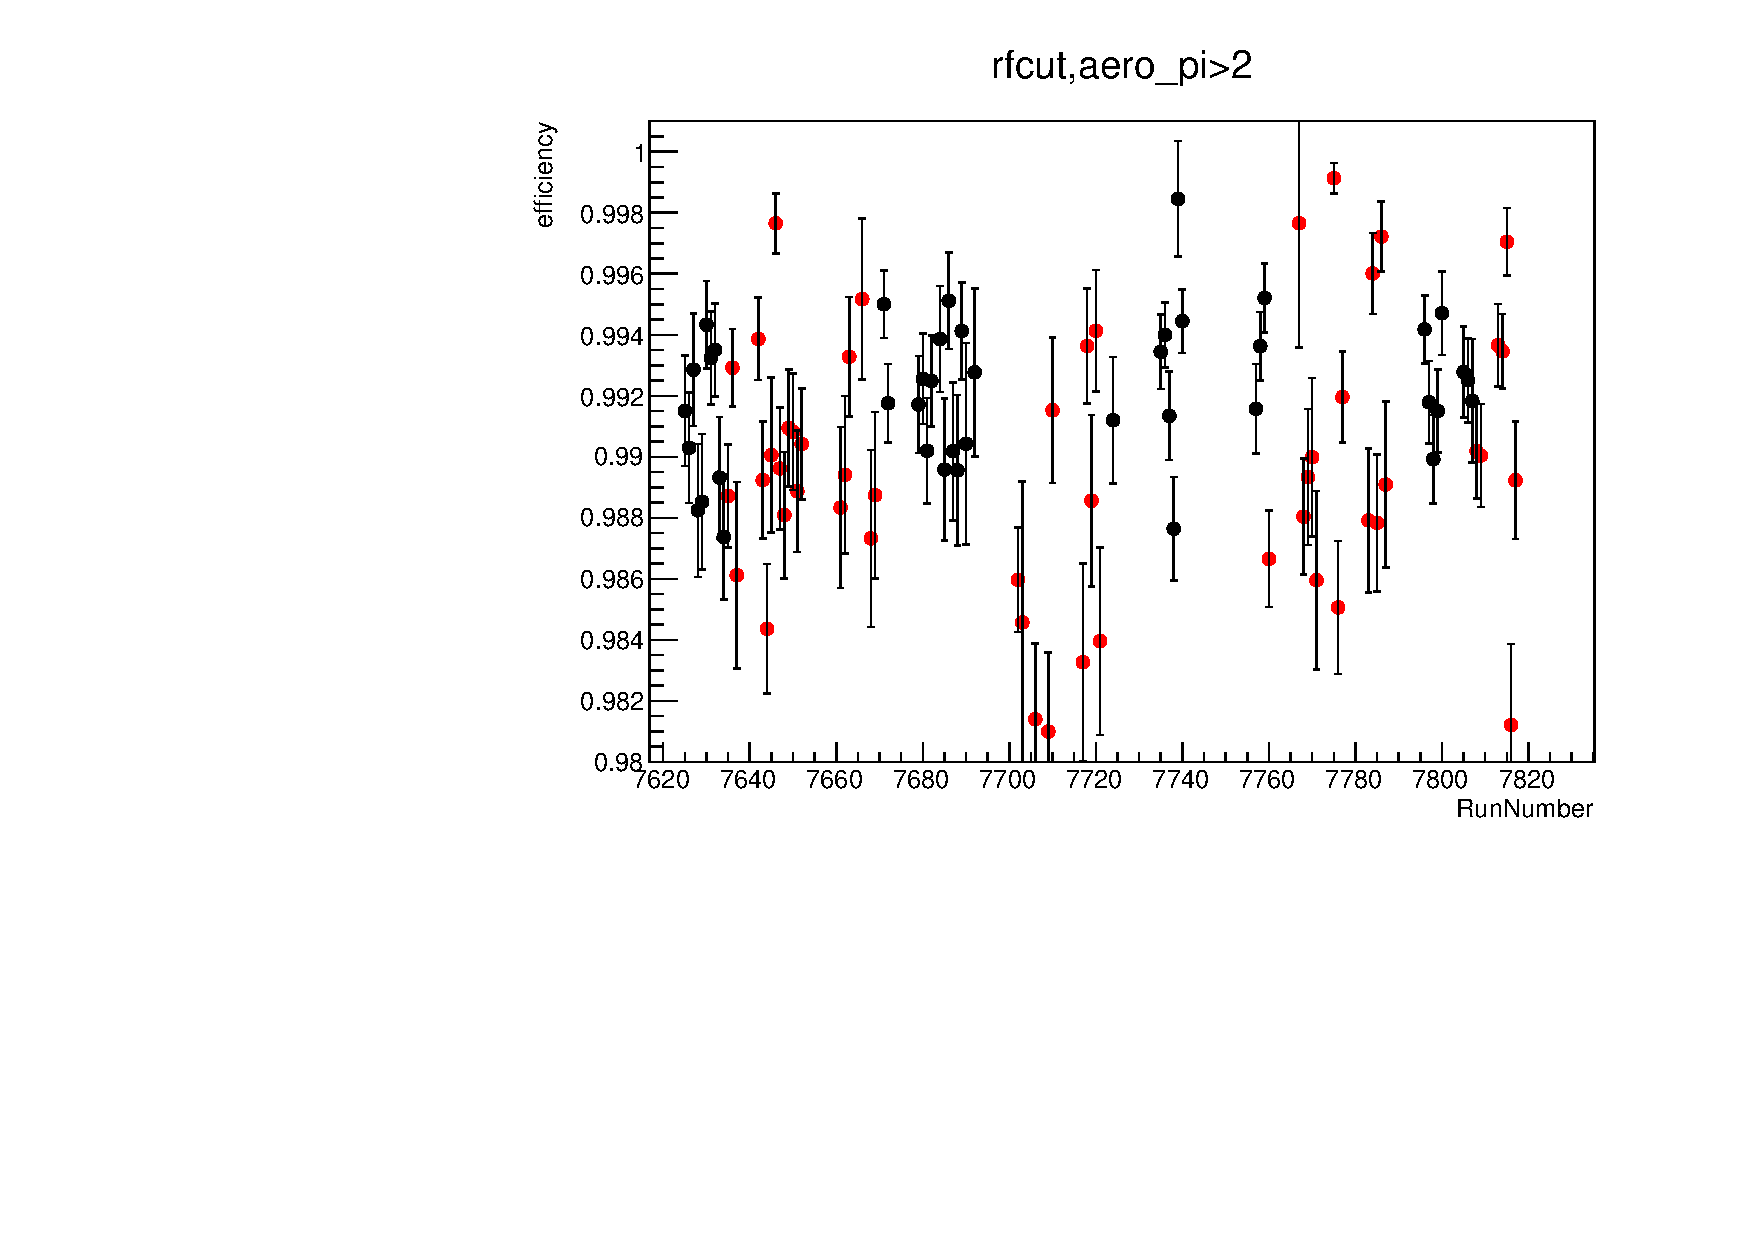
\includegraphics[width = 0.8\textwidth]{results/pid/SHMS_aero_DE_RunNumber_spring.pdf}
\end{frame}
\begin{frame}{SHMS aero efficiency verse RunGroup}
  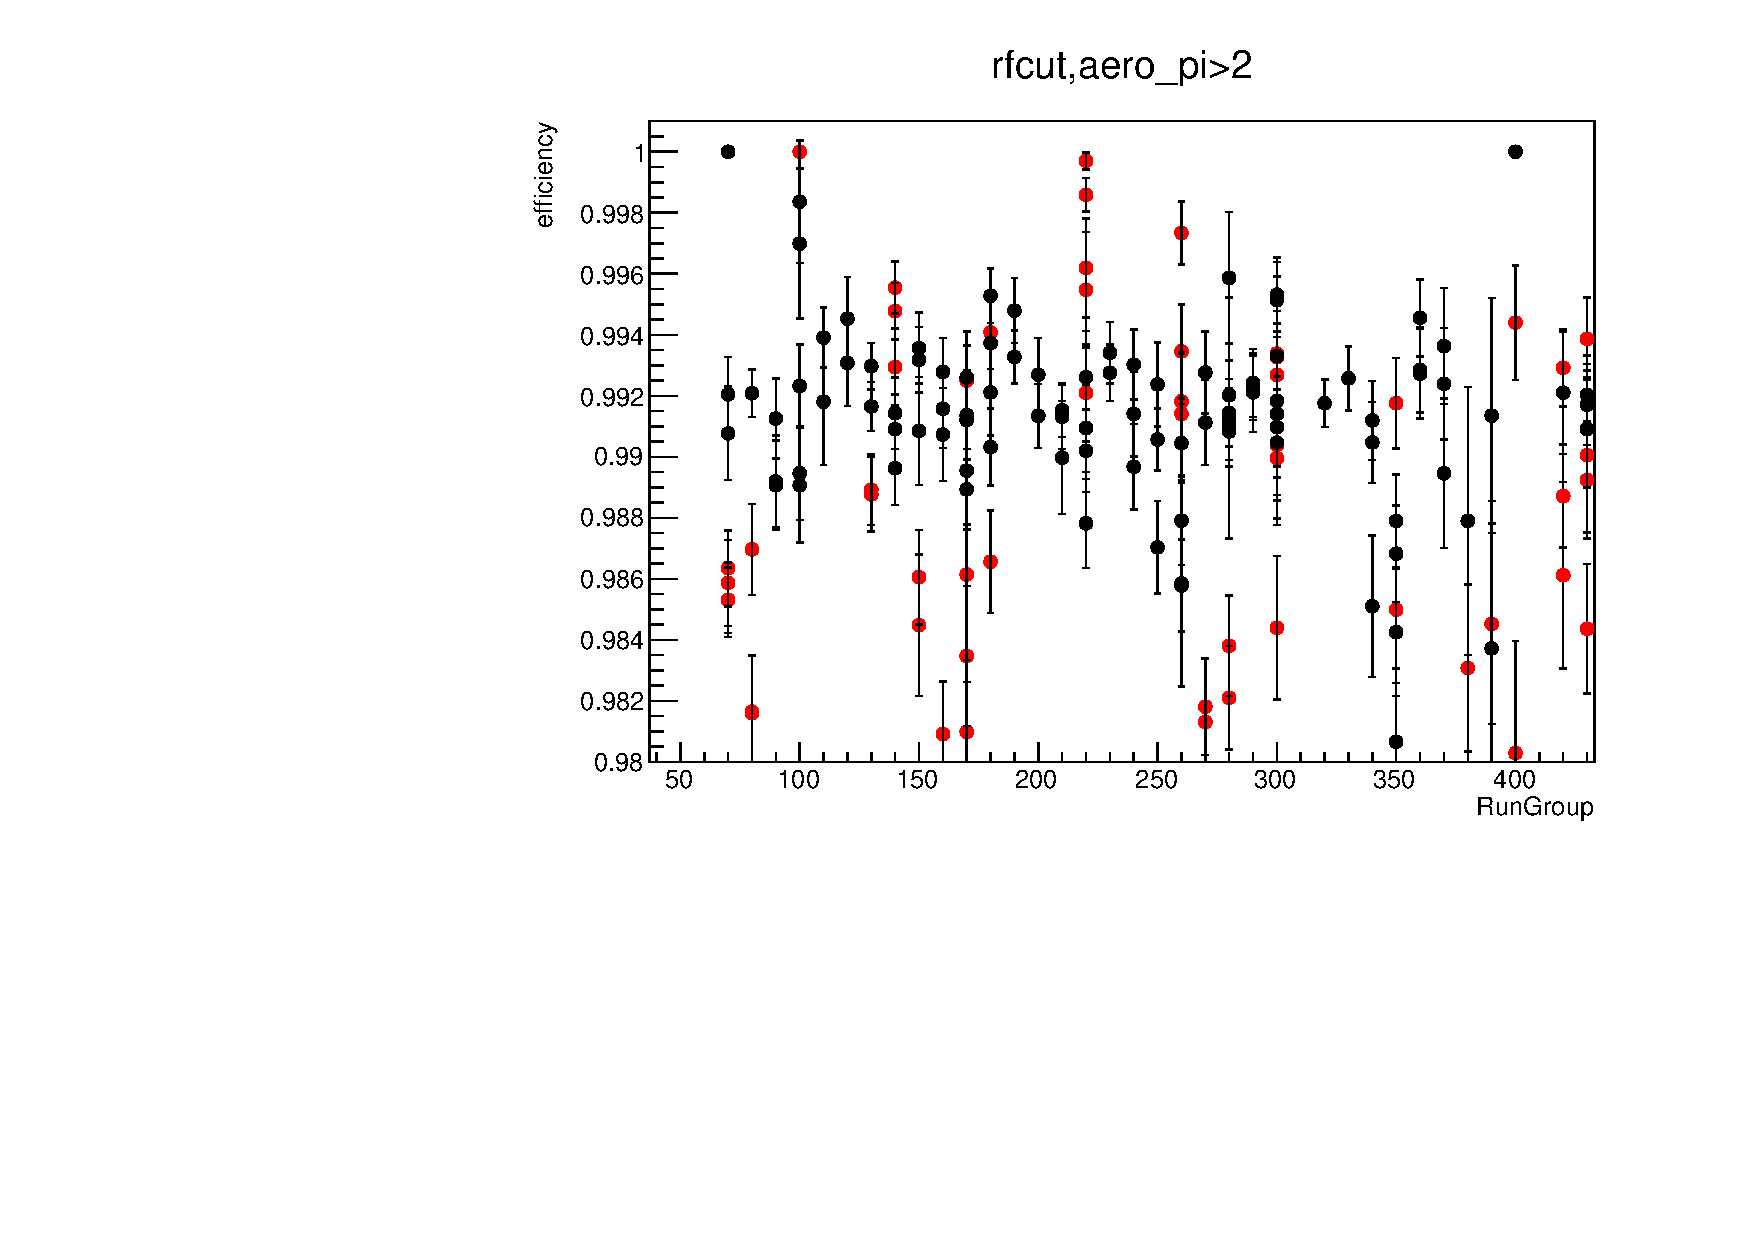
\includegraphics[width = 0.8\textwidth]{results/pid/SHMS_aero_DE_RunGroup.pdf}
\end{frame}

\begin{frame}{SHMS rftime cut, pion efficiency and kaon contamination}
  \begin{columns}
    \begin{column}[T]{0.5\textwidth}
      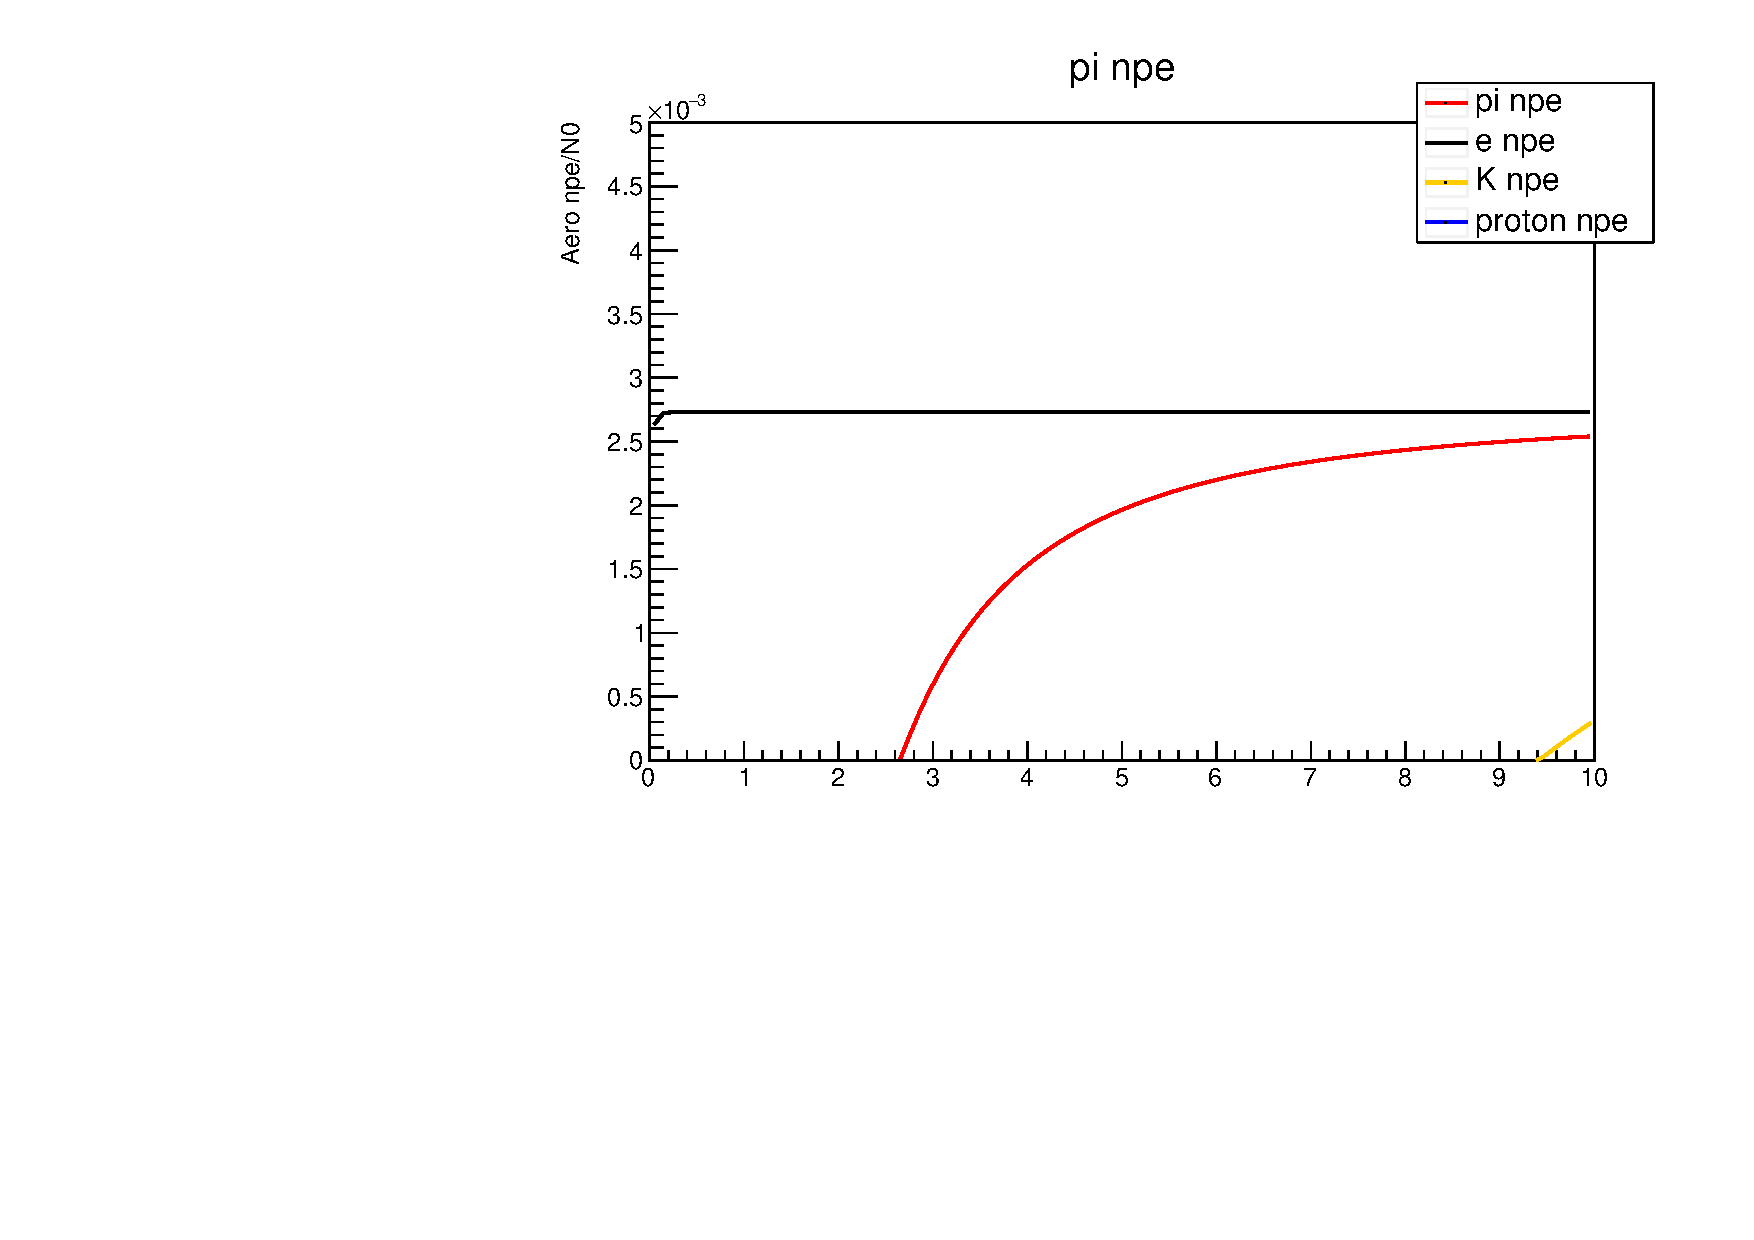
\includegraphics[width = 0.8\textwidth]{graphs/cerenkov/hgc_npe_p.pdf}
      \\
      hgcer npe verse momentum
    \end{column}
    \begin{column}[T]{0.5\textwidth}
      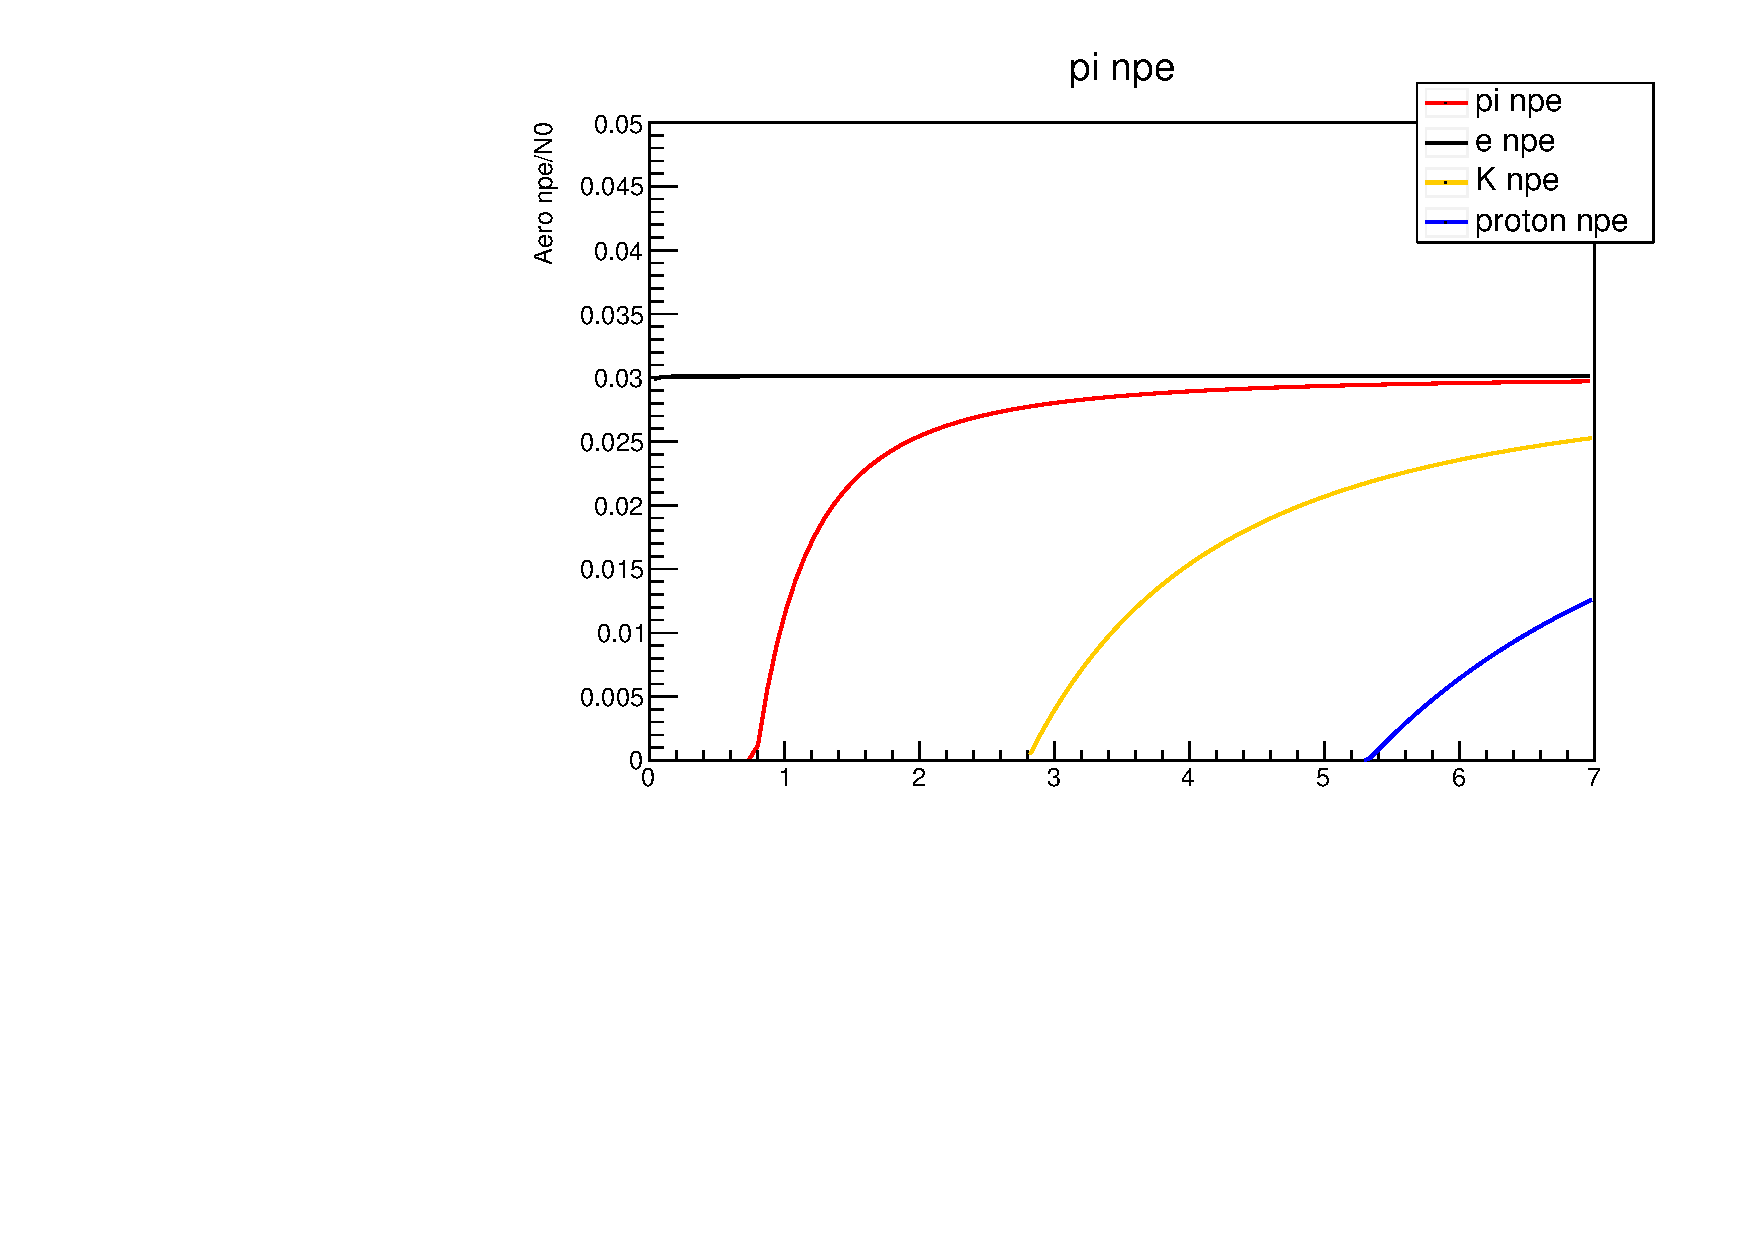
\includegraphics[width = 0.8\textwidth]{graphs/cerenkov/aero_npe_p.pdf}
      \\
      aero npe verse momentum
    \end{column}
  \end{columns}
\end{frame}
\begin{frame}{SHMS pion arm}
  \begin{block}{Basic cuts}
    cointime:2.5(fall)/1.5(spring) \\
    HMS(SHMS) delta:-8,8(-10,20) \\
    HMS(SHMS) acceptance constrain \\
    HMS e cut \\
    accidental background: 6 peaks \\
       Aerogel Cherenkov cut: 2 \\
       Calorimeter cut: 0.05,0.85
  \end{block}
     \begin{block}{SHMS rftiming}
       0.5,1.5 \\ 
       -3\sigma, 3\sigma
     \end{block}
  %\begin{center}
  %  \begin{tabular}{|c|c|c|c|c|c|}
  %    \hline
  %    Cuts & HMS cal &HMS cer &  SHMS cal & SHMS aero & SHMS rf \\
  %    \hline
  %    cointime & 1.5/2.5 & same & same & same & same\\
  %    \hline
  %    H dp & -8,8 & same & same & same & same\\
  %    \hline
  %    P dp & -10,20 & same & same & same & same\\
  %    \hline
  %    H xptar & -0.06,0.06 & same & same & same & same\\
  %    \hline
  %    H yptar & -0.022,0.022 & same & same & same & same\\
  %    \hline
  %    P xptar & -0.045,0.045 & same & same & same & same\\ 
  %    \hline
  %    P yptar & -0.028,0.028 & same & same & same & same\\
  %    \hline
  %    bg & -3,+3 & same & same & same & same\\
  %    \hline
  %    P cal & 0.05,0.85 &same & varies & 0.05,0.85 & same \\
  %    \hline
  %    P hgcer & non &non& non & non & \< 2\\
  %    \hline
  %    P rf & 0.5,1.5 &same& same &same & varies\\
  %    \hline
  %    P aero & 2 &same & same & varies & \> 10\\
  %    \hline
  %    H cal & varies & 1 & 0.8 & same & same \\
  %    \hline 
  %    H cer & 12 & varies & 2 & same & same \\
  %    \hline
  %  \end{tabular}
  %\end{center}

\end{frame}

\begin{frame}{rf cut, pion efficiency and kaon contamination}
  \begin{columns}
    \begin{column}[T]{0.5\textwidth}
  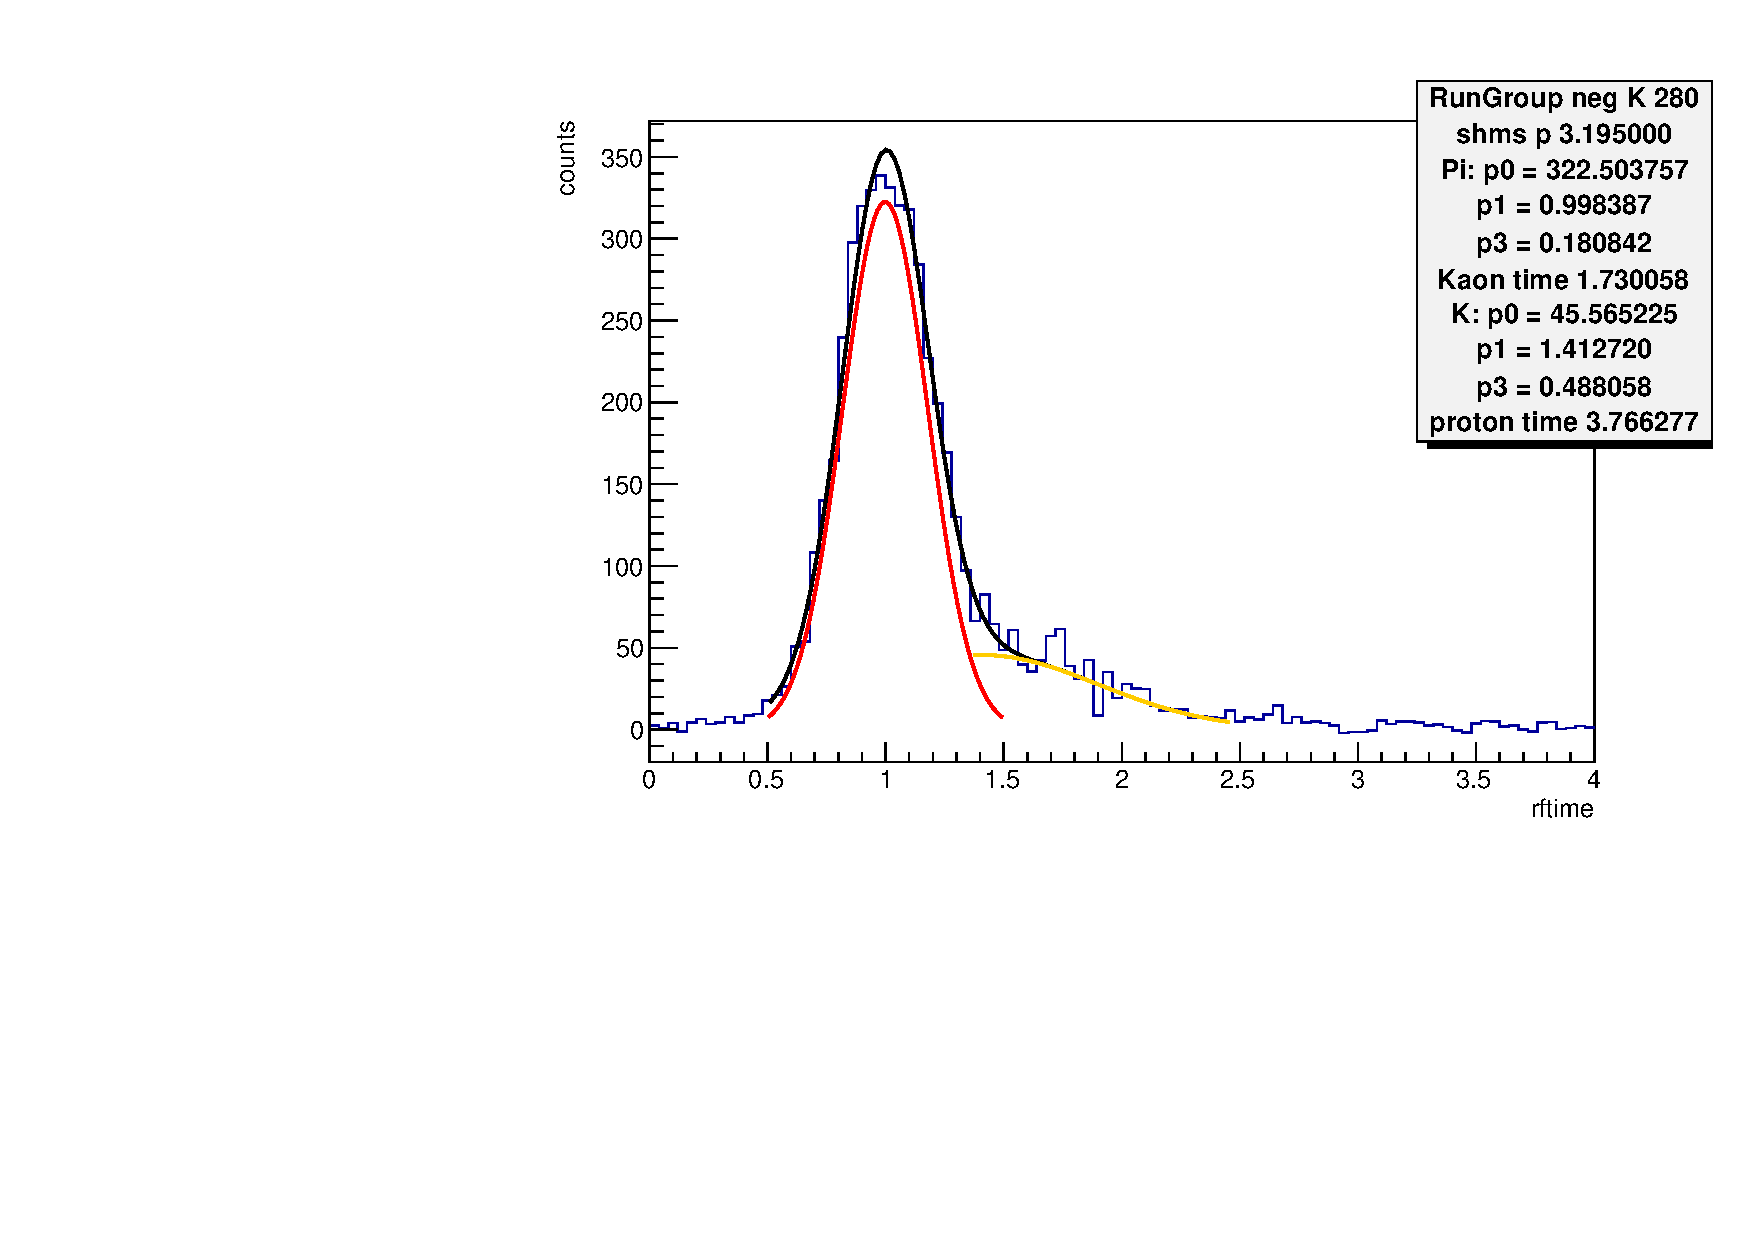
\includegraphics[width = 0.8\textwidth]{results/pid/rftime/rftime_neg_280.pdf}
\end{column}
\begin{column}[T]{0.5\textwidth}
  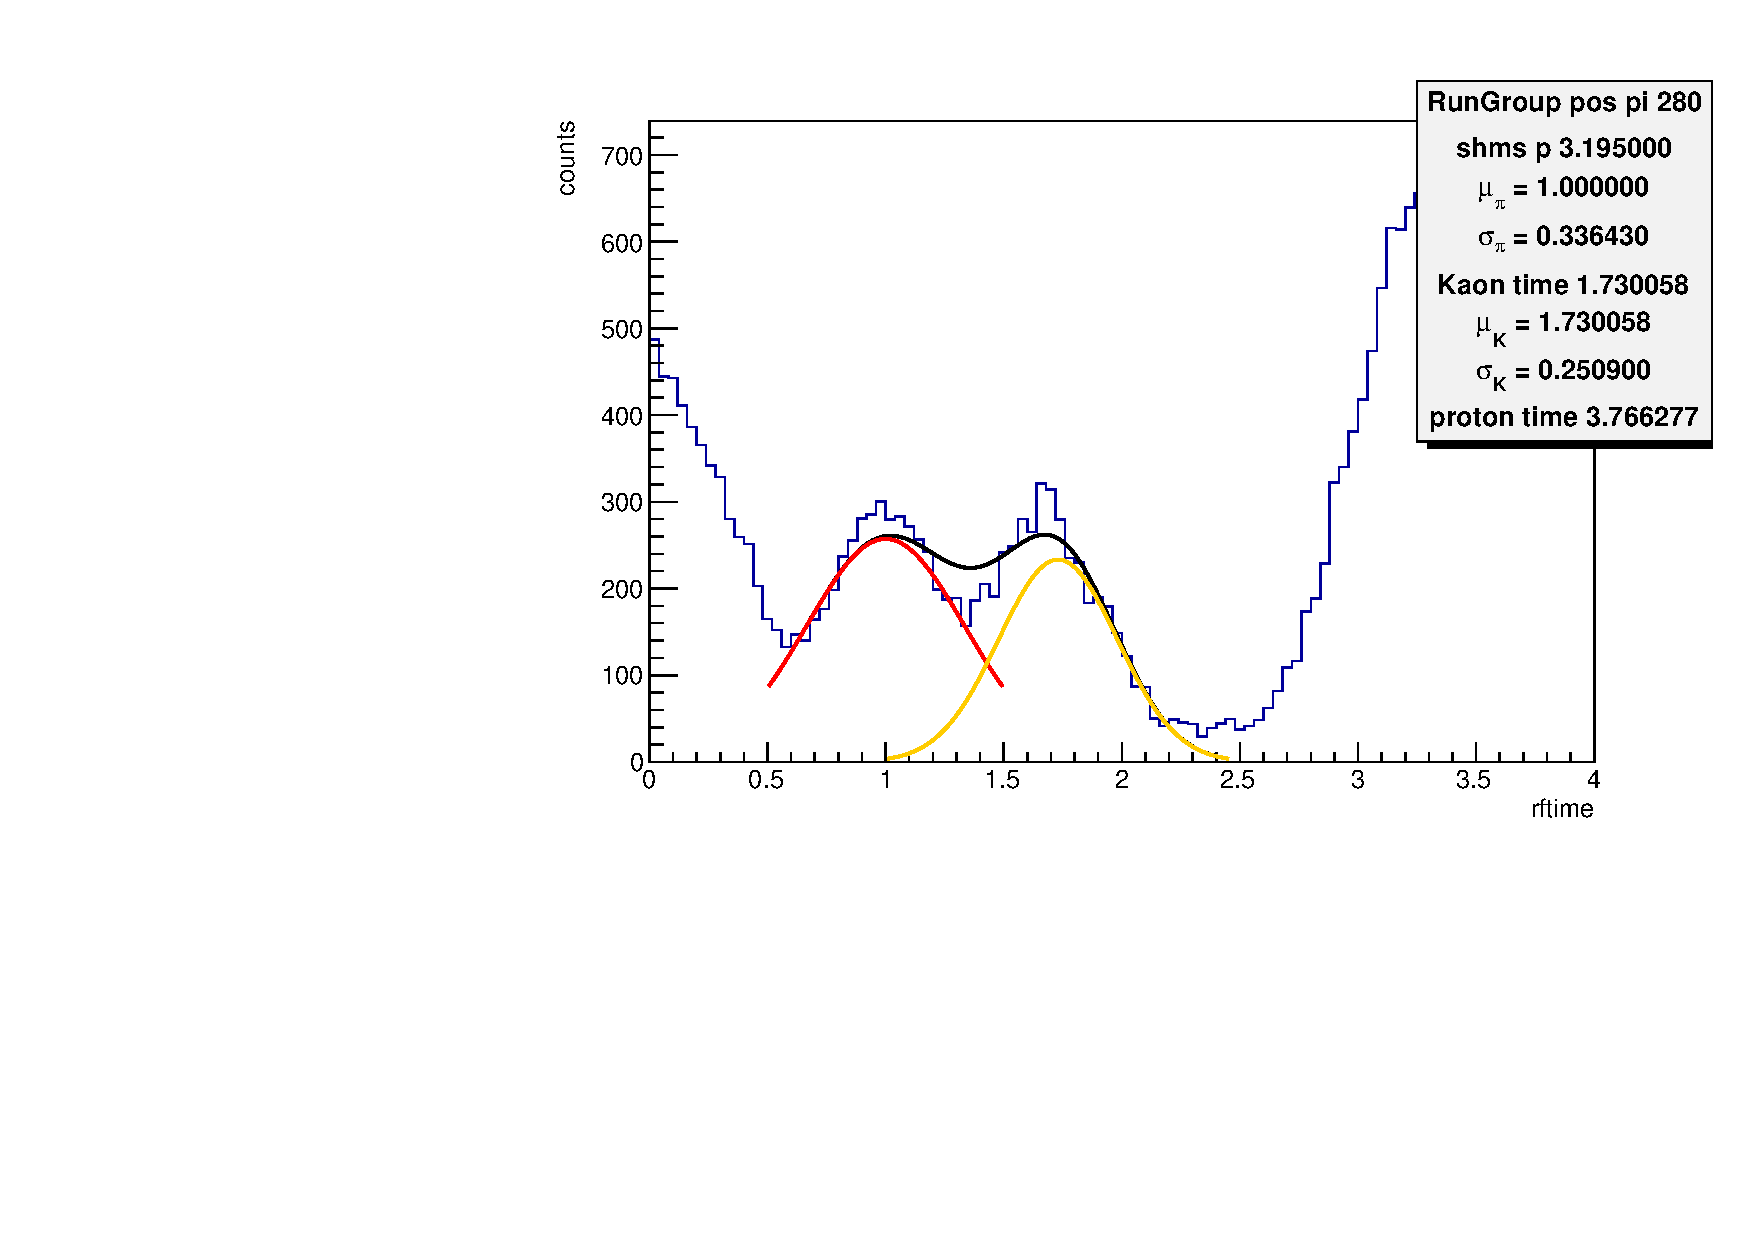
\includegraphics[width = 0.8\textwidth]{results/pid/rftime/rftime_pos_280.pdf}
\end{column}
\end{columns}
\\
HGcer greater than 2. Cut pions to show kaons here. 
\end{frame}
\begin{frame}{rf cut, pion efficiency and kaon contamination}
  \begin{columns}
    \begin{column}[T]{0.5\textwidth}
  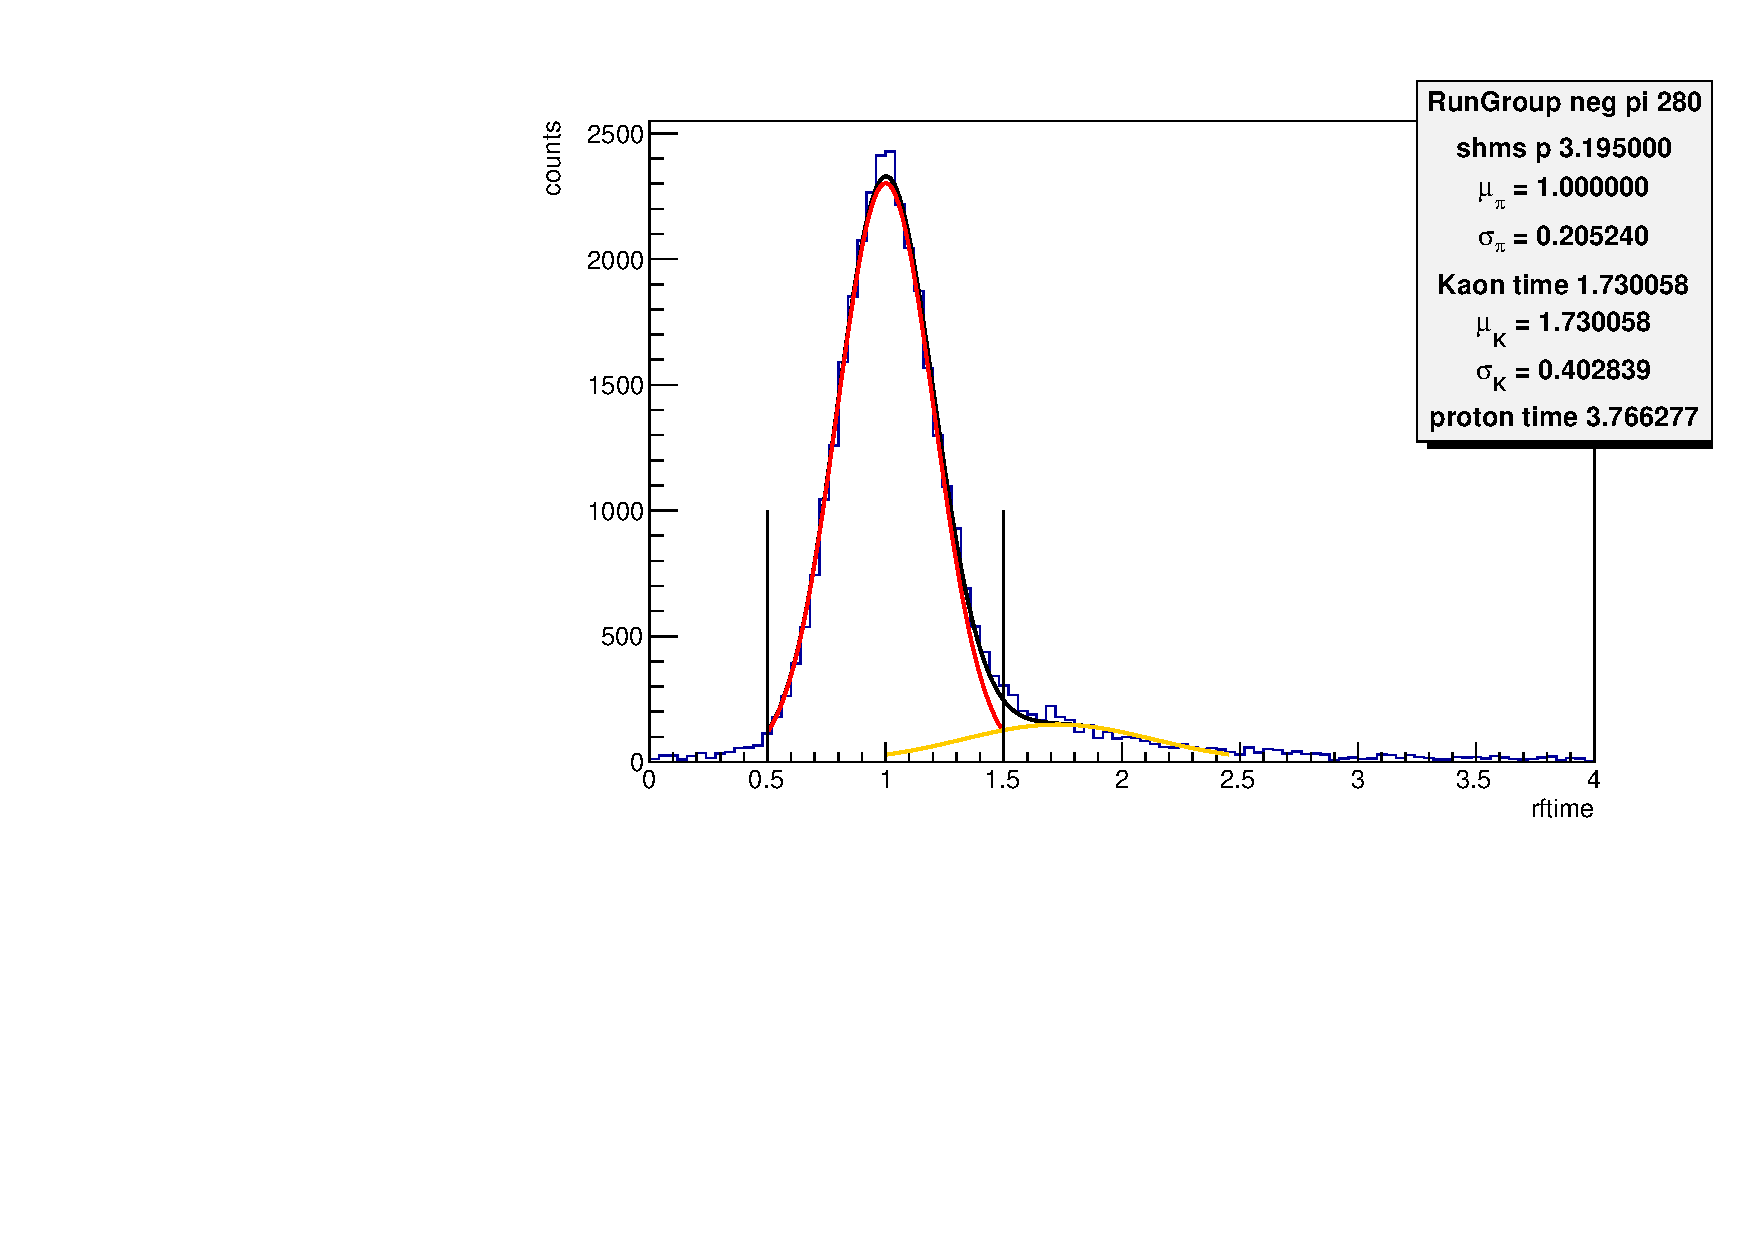
\includegraphics[width = 0.8\textwidth]{results/pid/rftime/rftime_neg_280_pi.pdf}
\end{column}
\begin{column}[T]{0.5\textwidth}
  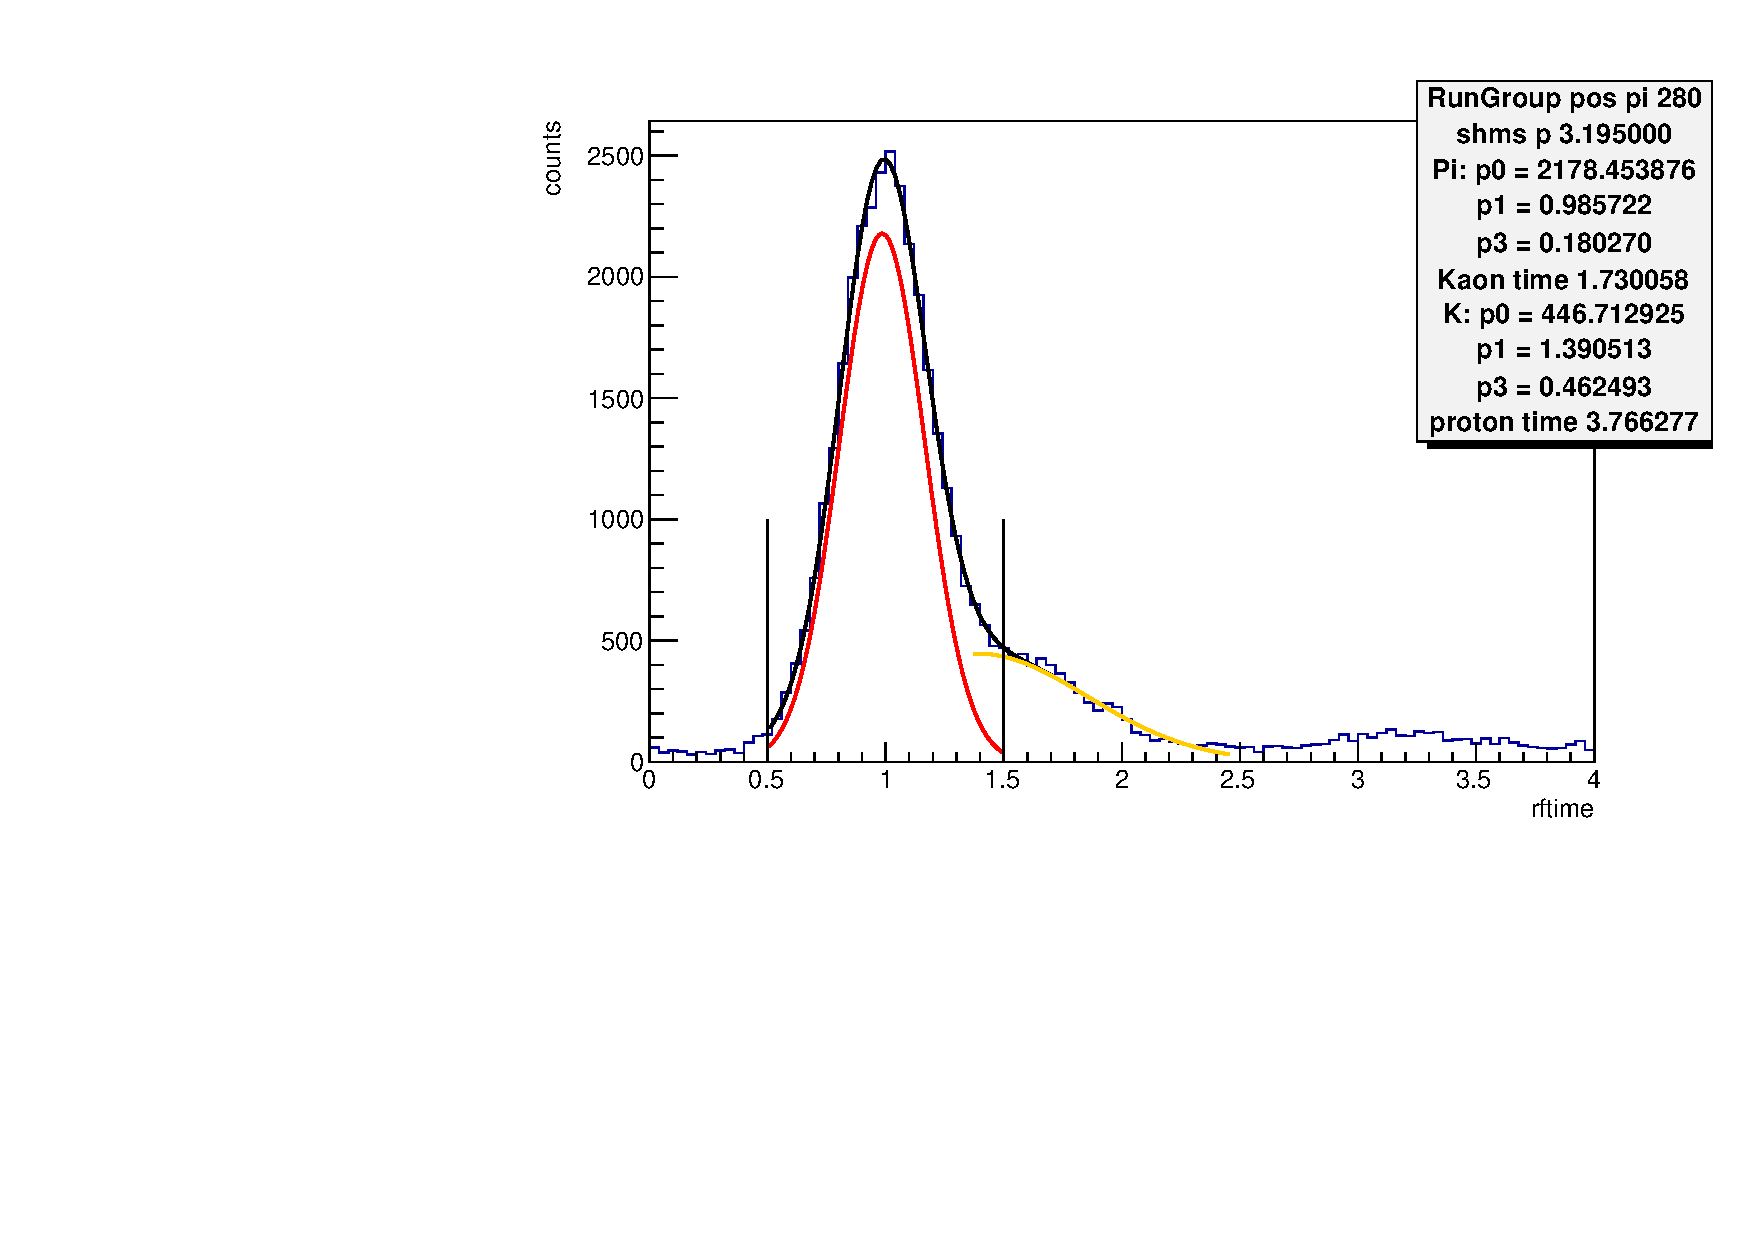
\includegraphics[width = 0.8\textwidth]{results/pid/rftime/rftime_pos_280_pi.pdf}
\end{column}
\end{columns}
\\
pi\_eff from gaussian distribution
\\
kaon con = $\frac{kaon fit integral[rfcut]}{all fit integral [rfcut]}$
\end{frame}
\begin{frame}{rf cut, pion efficiency and kaon contamination}
  \begin{columns}
    \begin{column}[T]{0.5\textwidth}
  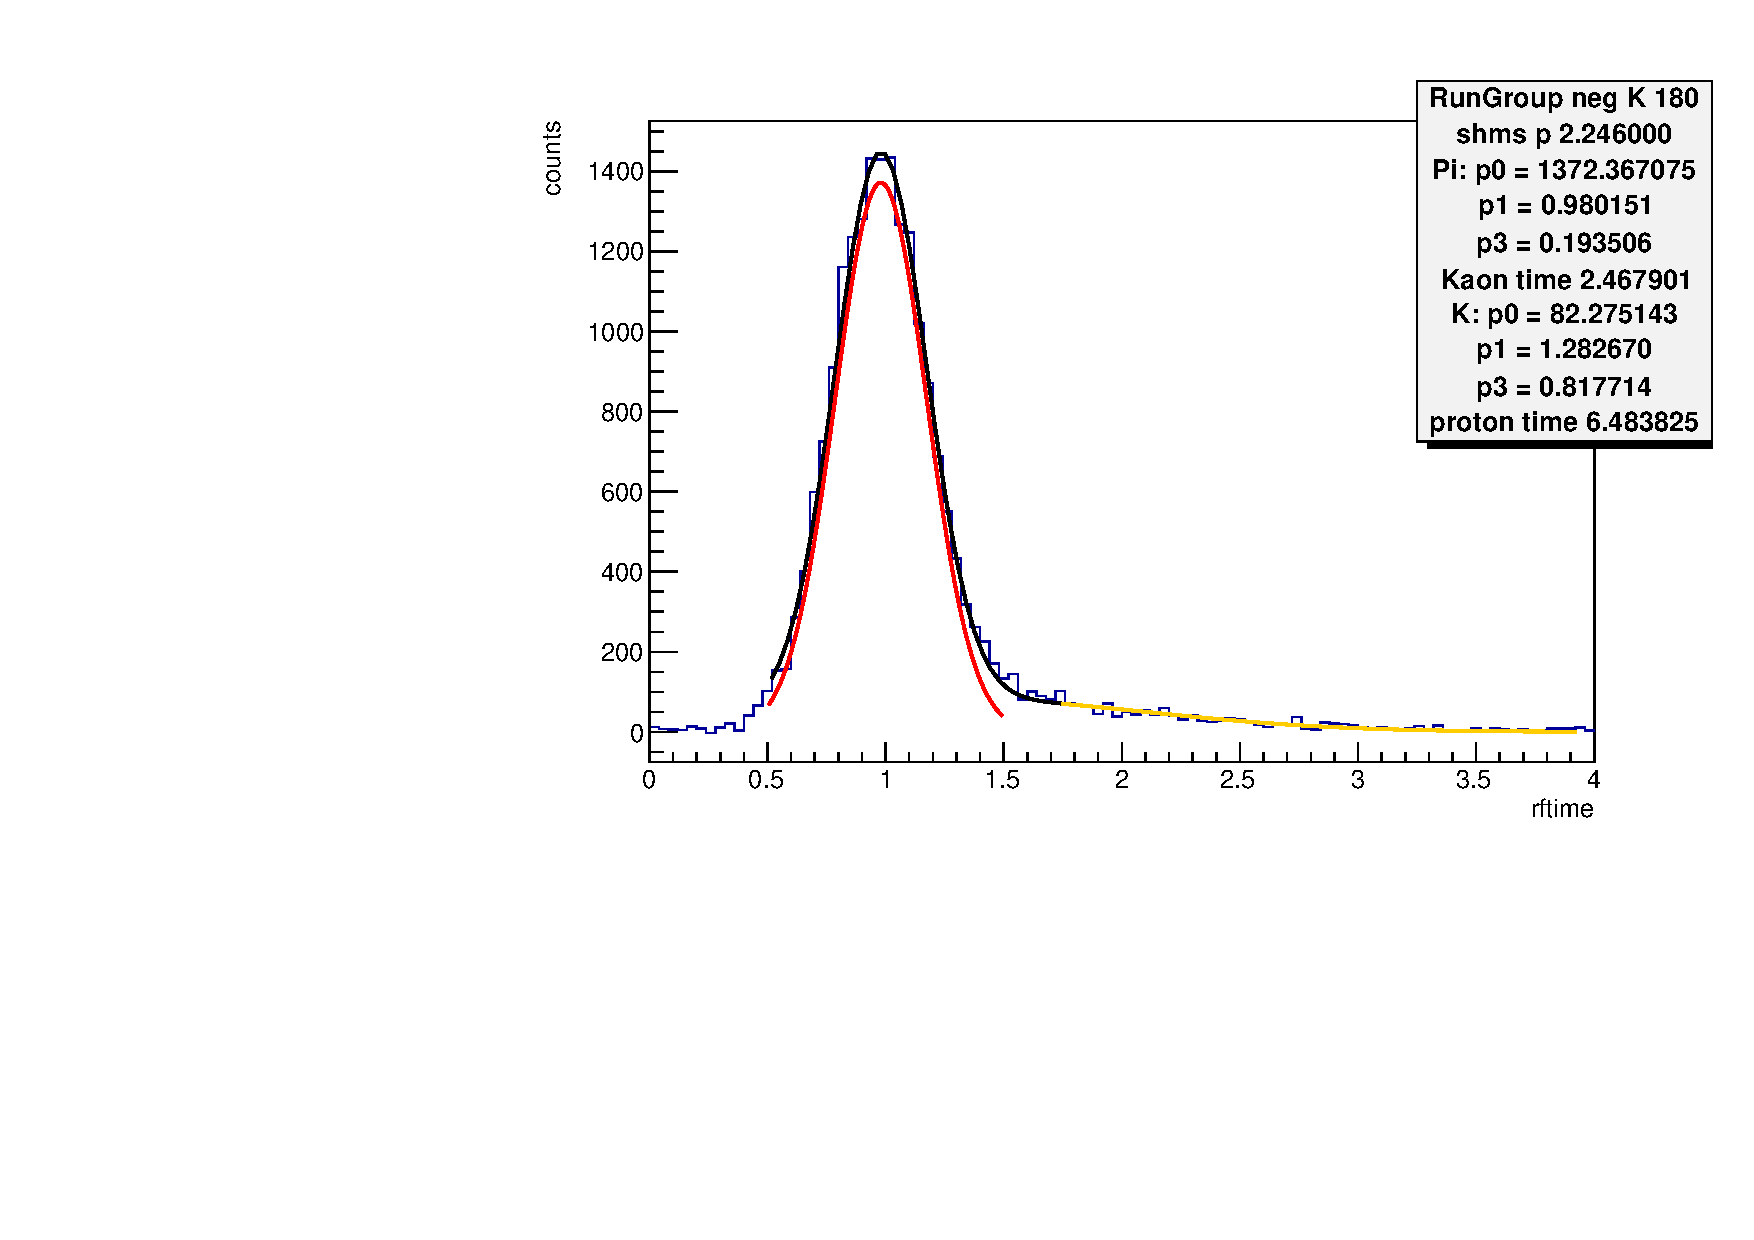
\includegraphics[width = 0.8\textwidth]{results/pid/rftime/rftime_neg_180.pdf}
\end{column}
\begin{column}[T]{0.5\textwidth}
  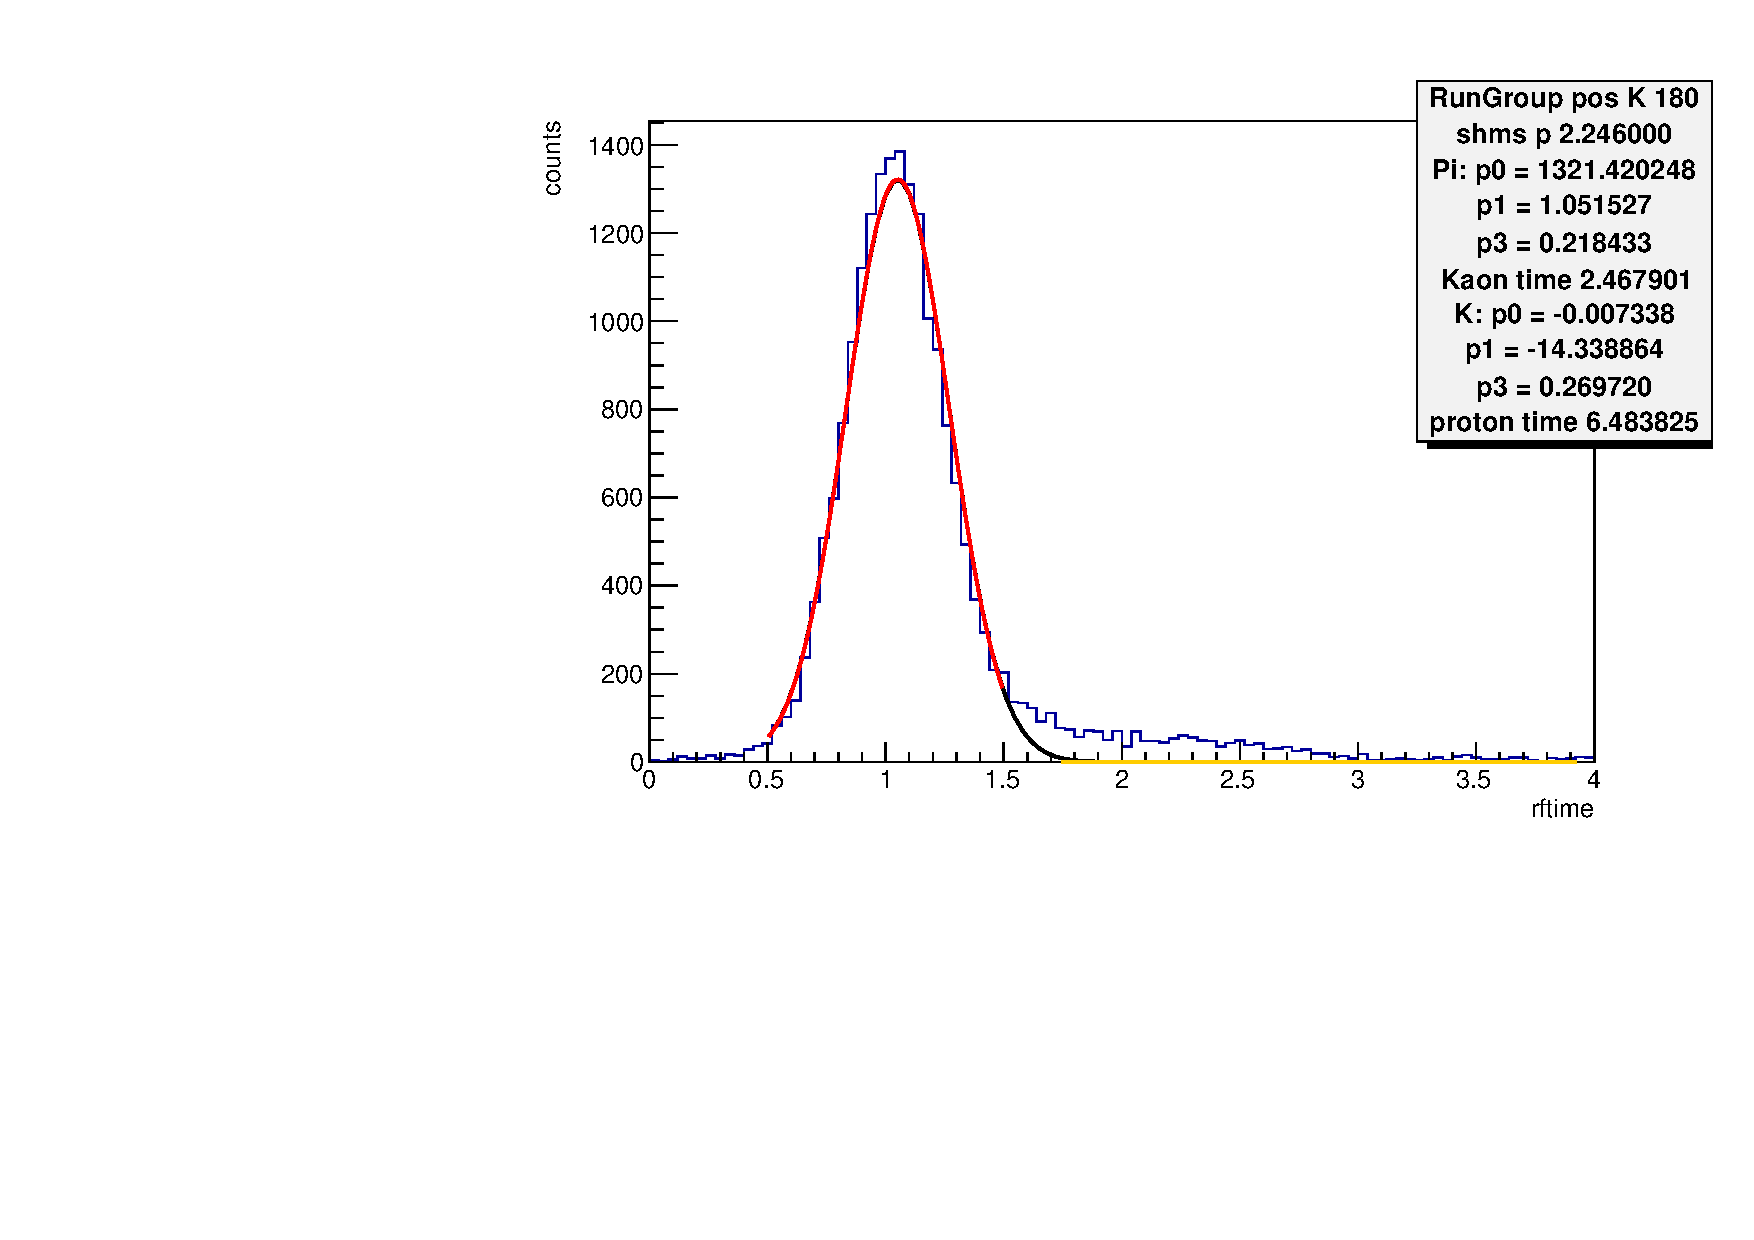
\includegraphics[width = 0.8\textwidth]{results/pid/rftime/rftime_pos_180.pdf}
\end{column}
\end{columns}
\\
HGcer greater than 2. Cut pions to show kaons here.
\end{frame}
\begin{frame}{rf cut, pion efficiency and kaon contamination}
  \begin{columns}
    \begin{column}[T]{0.5\textwidth}
  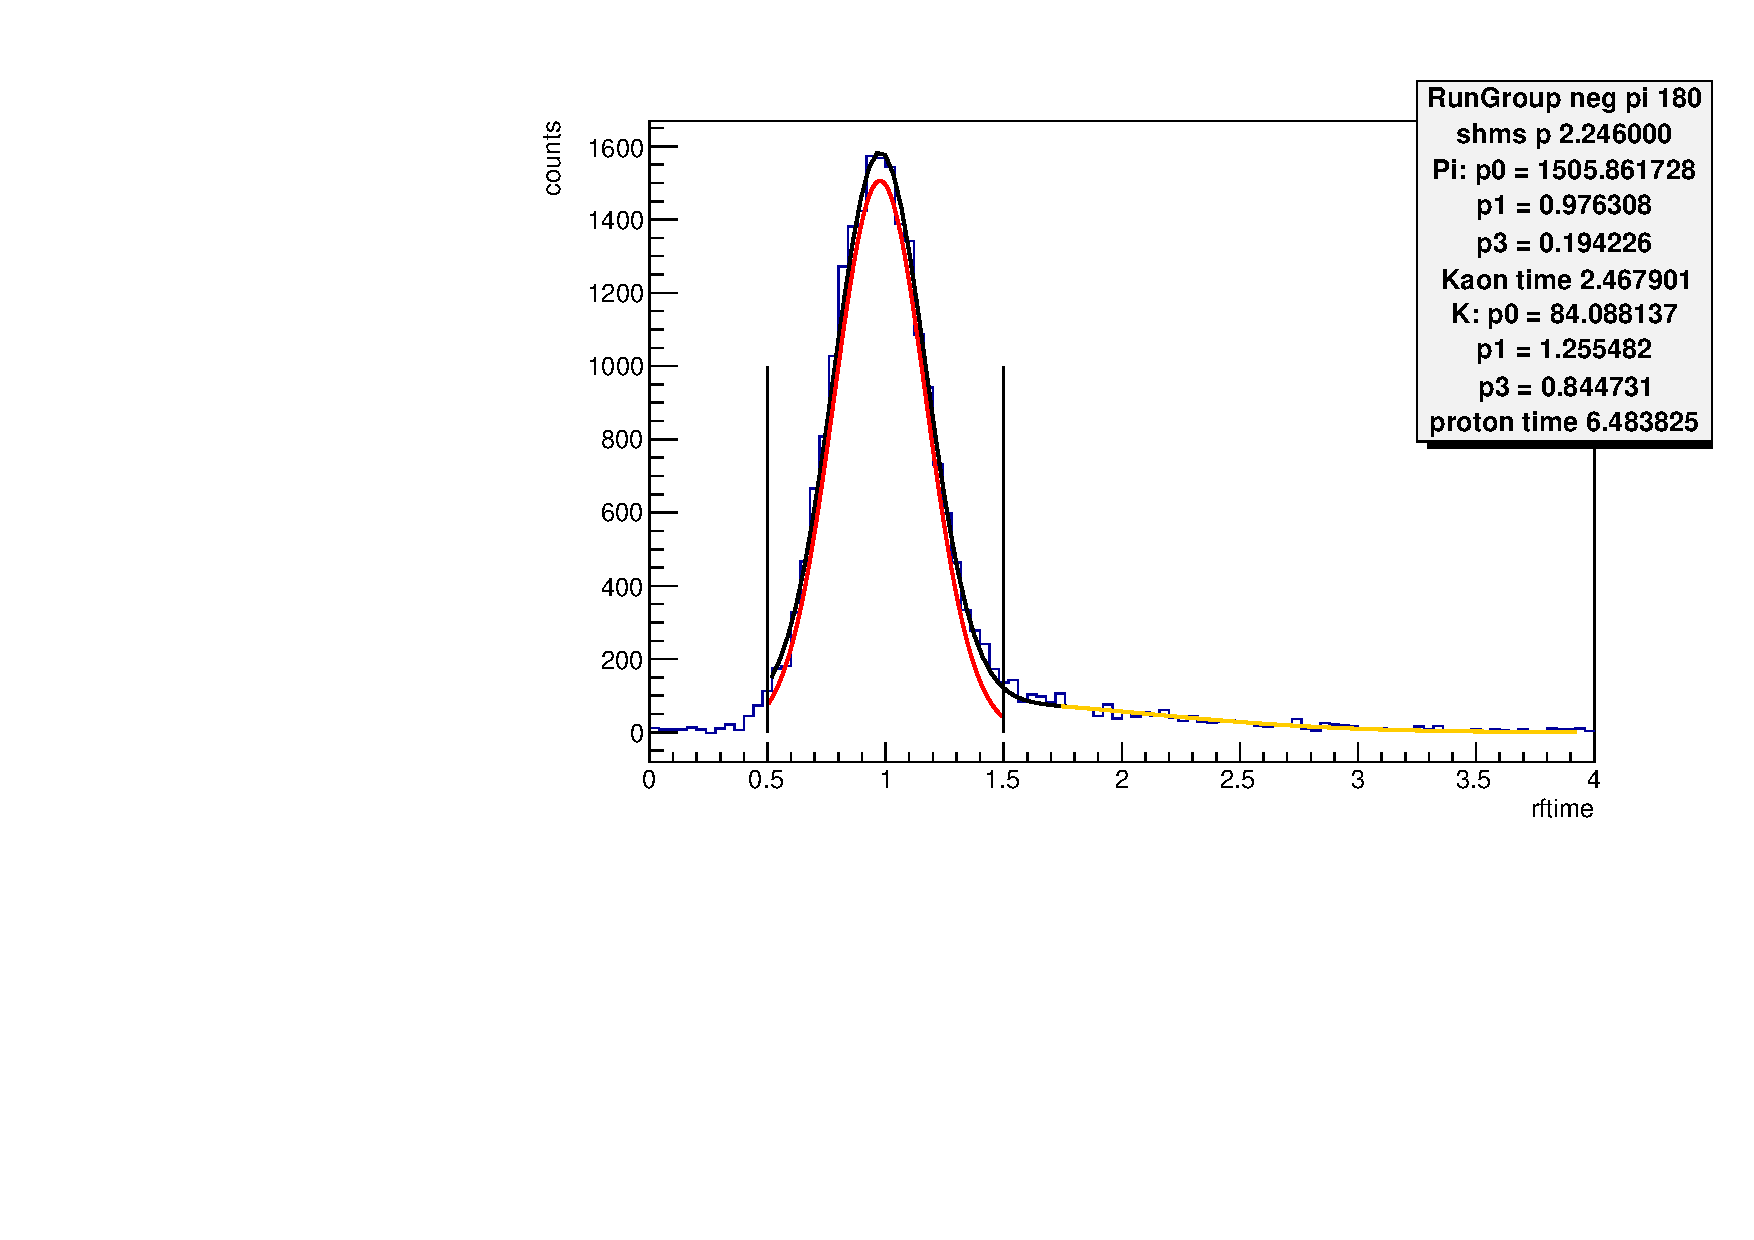
\includegraphics[width = 0.8\textwidth]{results/pid/rftime/rftime_neg_180_pi.pdf}
\end{column}
\begin{column}[T]{0.5\textwidth}
  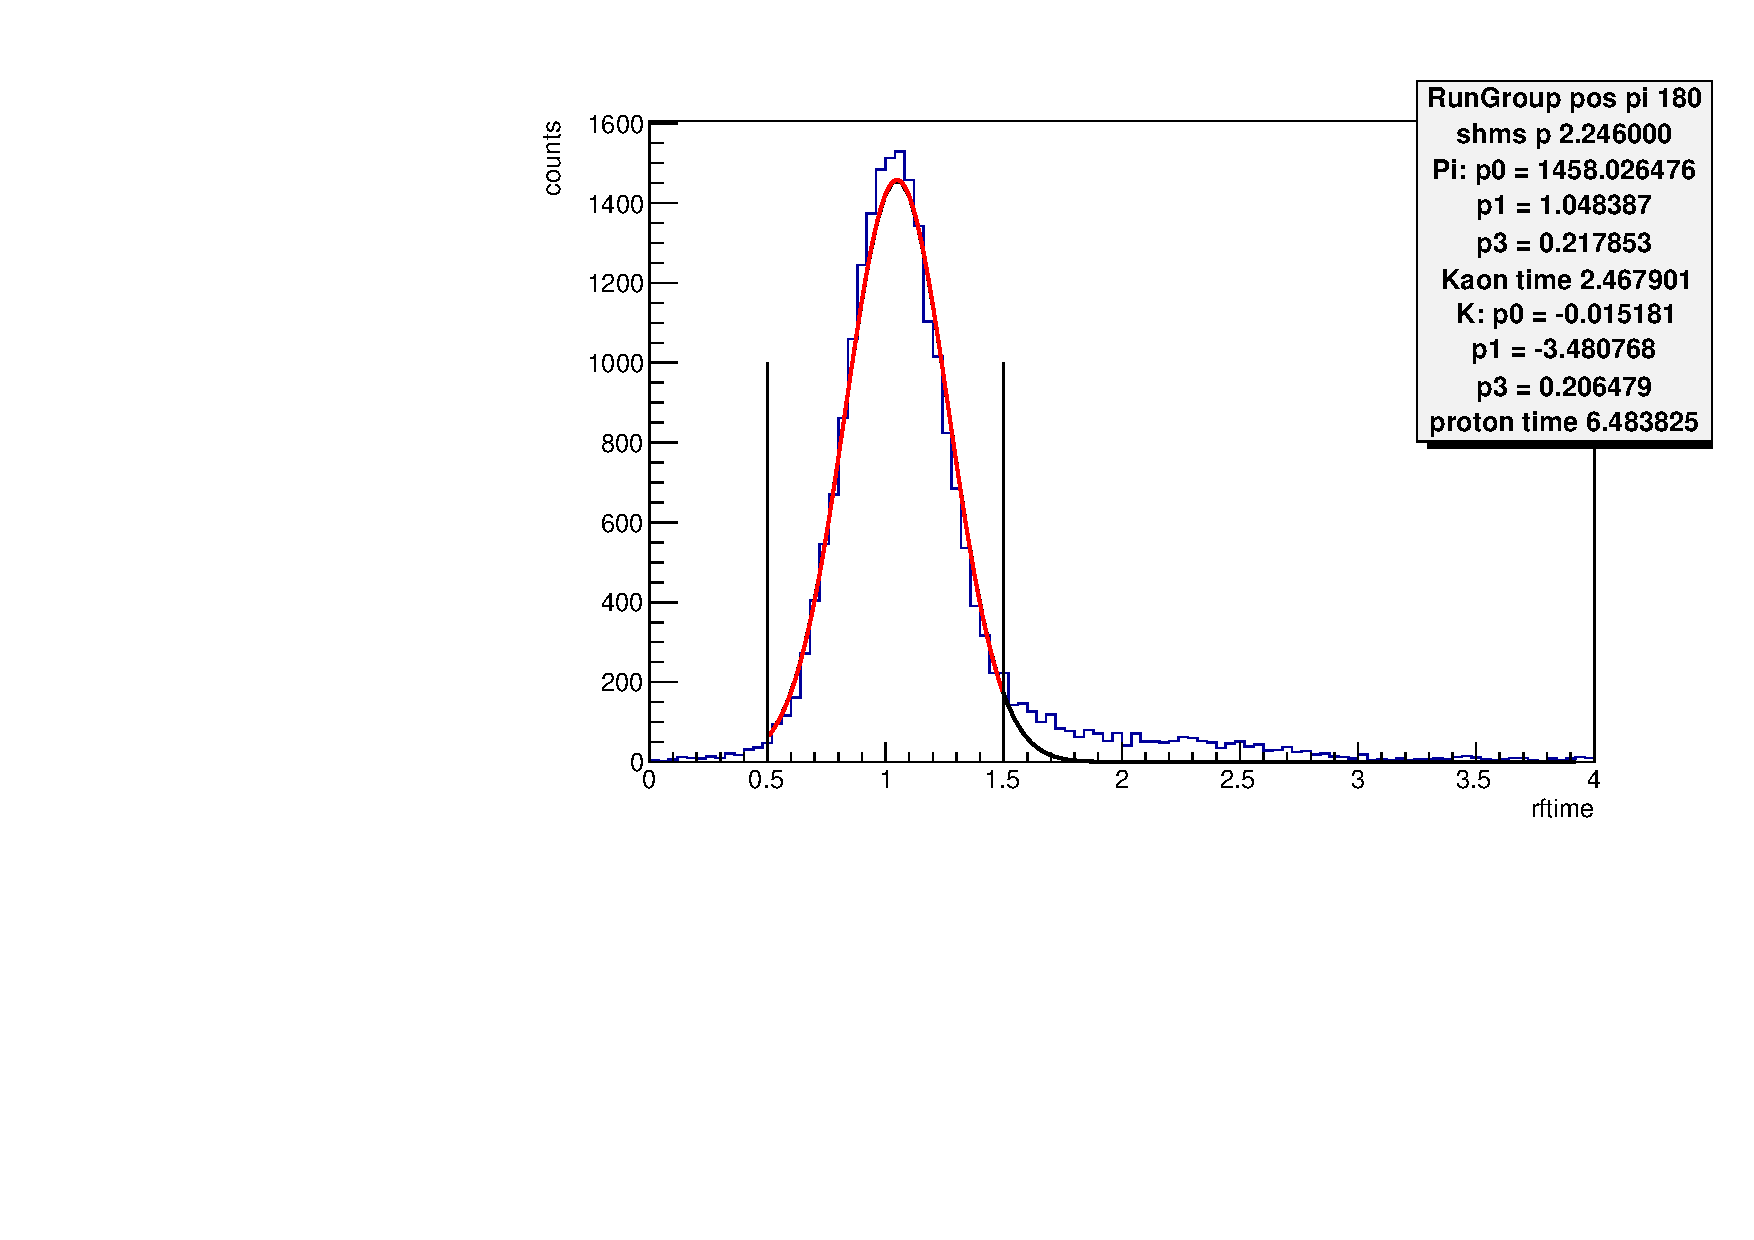
\includegraphics[width = 0.8\textwidth]{results/pid/rftime/rftime_pos_180_pi.pdf}
\end{column}
\end{columns}
\end{frame}
\begin{frame}{rf cut, pion efficiency and kaon contamination}
  \begin{columns}
    \begin{column}[T]{0.5\textwidth}
  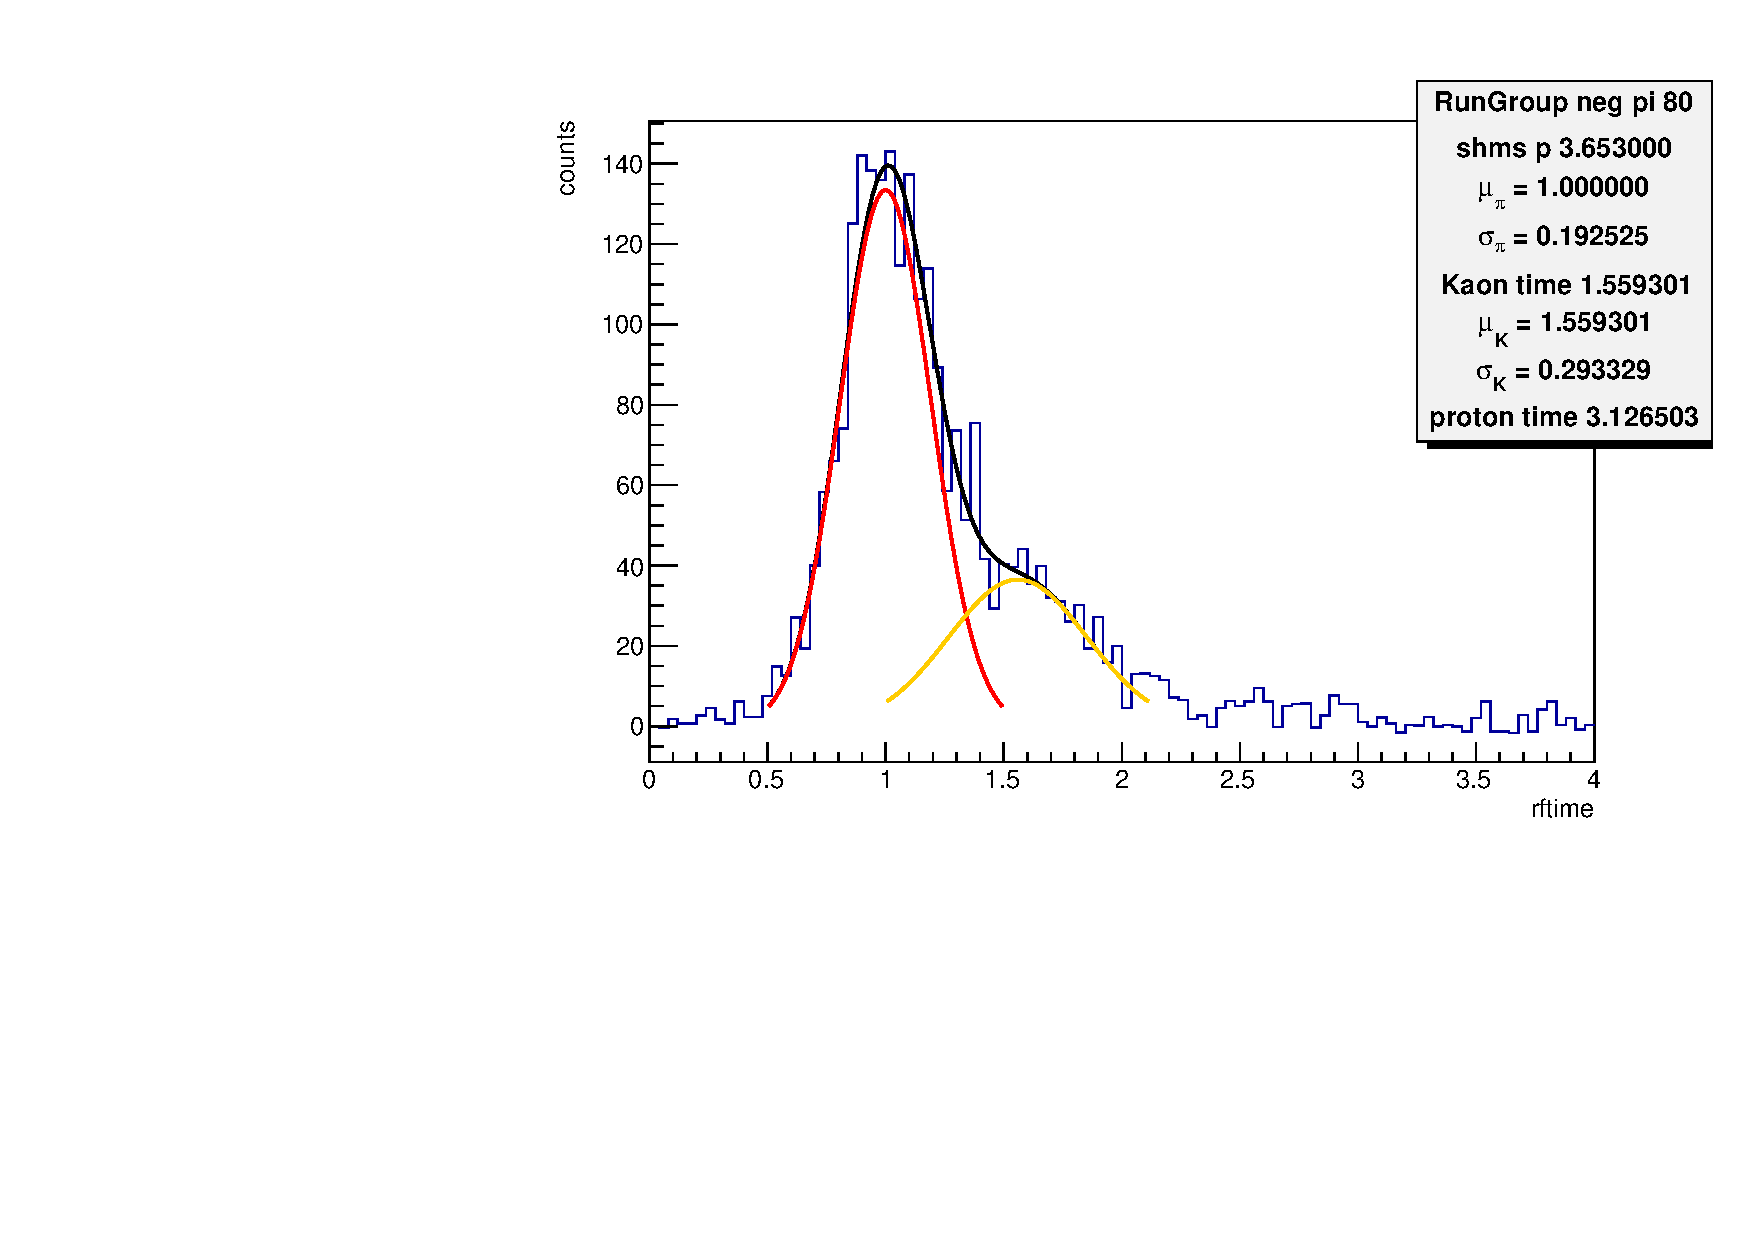
\includegraphics[width = 0.8\textwidth]{results/pid/rftime/rftime_neg_80.pdf}
\end{column}
\begin{column}[T]{0.5\textwidth}
  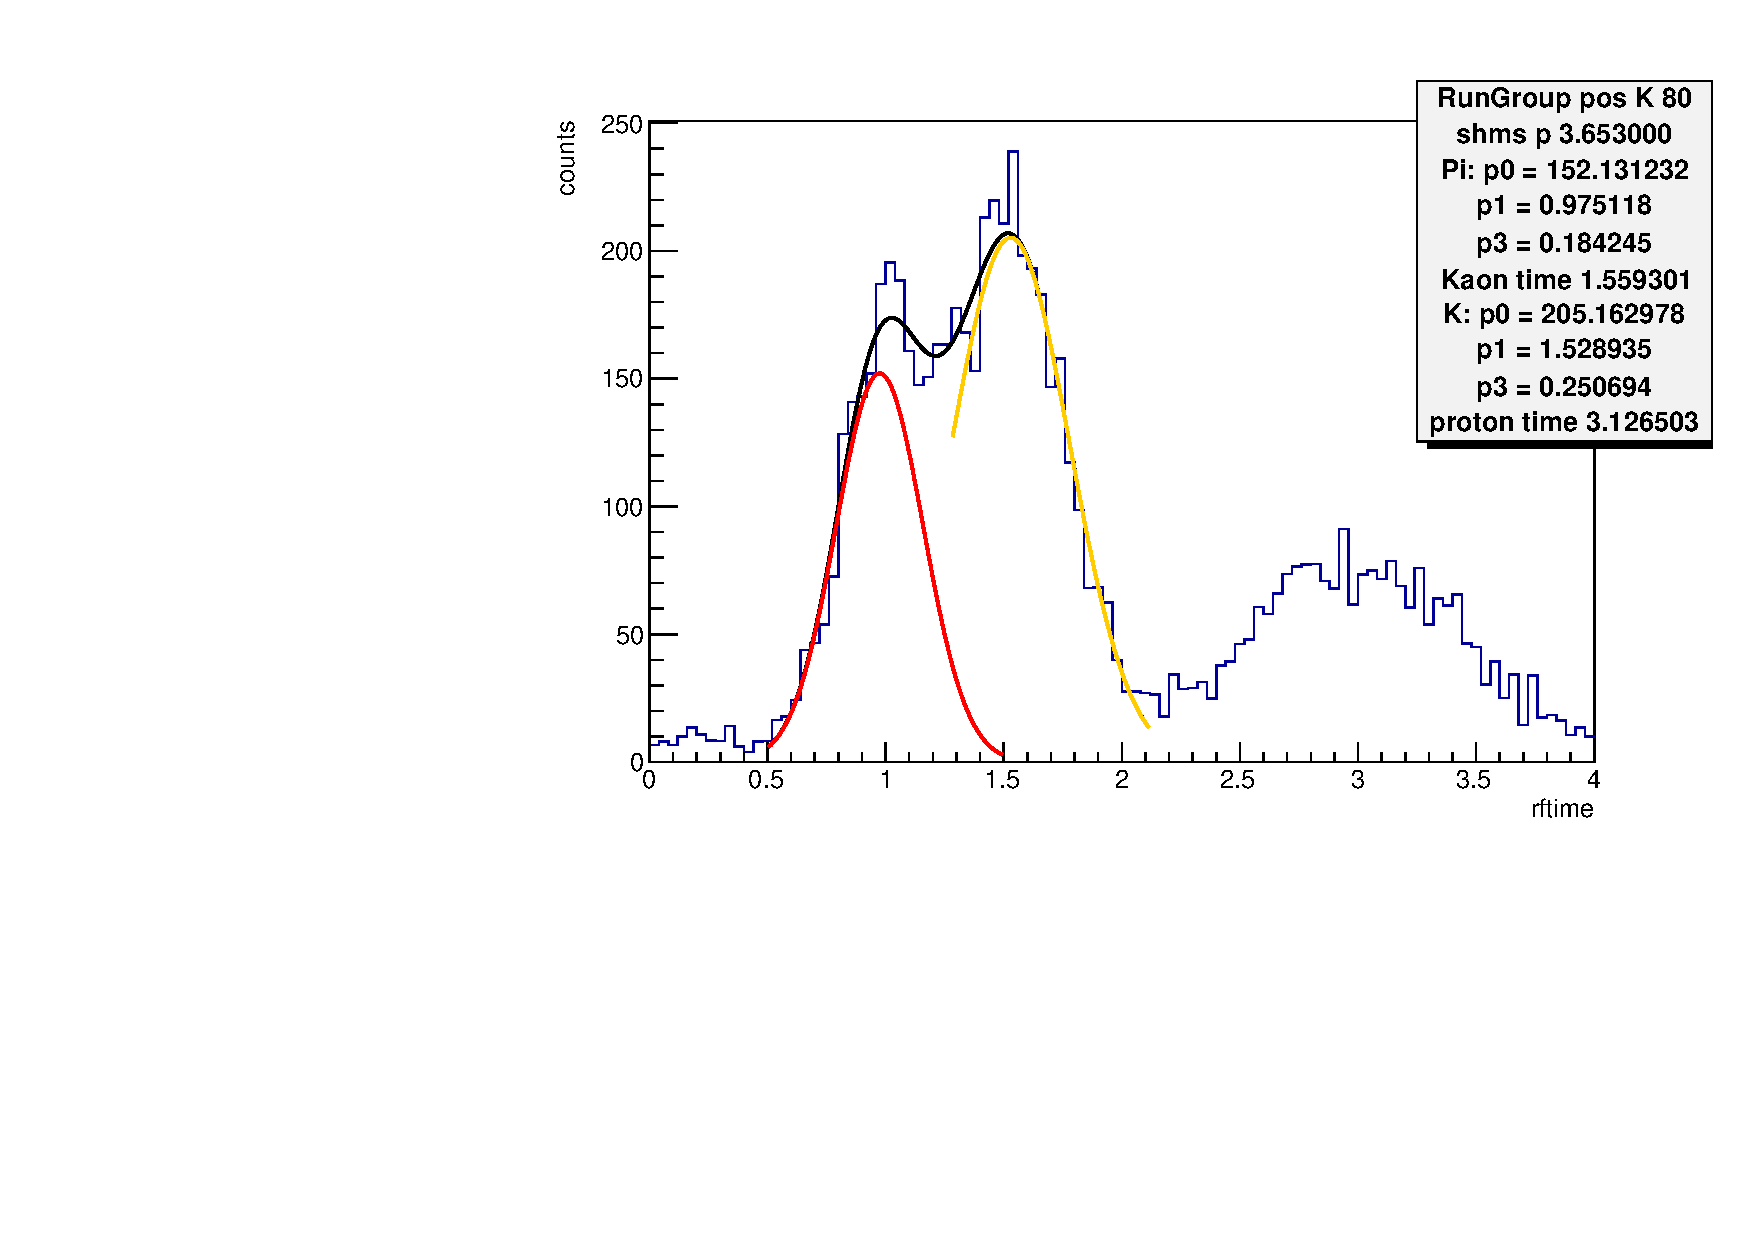
\includegraphics[width = 0.8\textwidth]{results/pid/rftime/rftime_pos_80.pdf}
\end{column}
\end{columns}
\\
HGcer greater than 2. Cut pions to show kaons here.
\end{frame}
\begin{frame}{rf cut, pion efficiency and kaon contamination}
  \begin{columns}
    \begin{column}[T]{0.5\textwidth}
  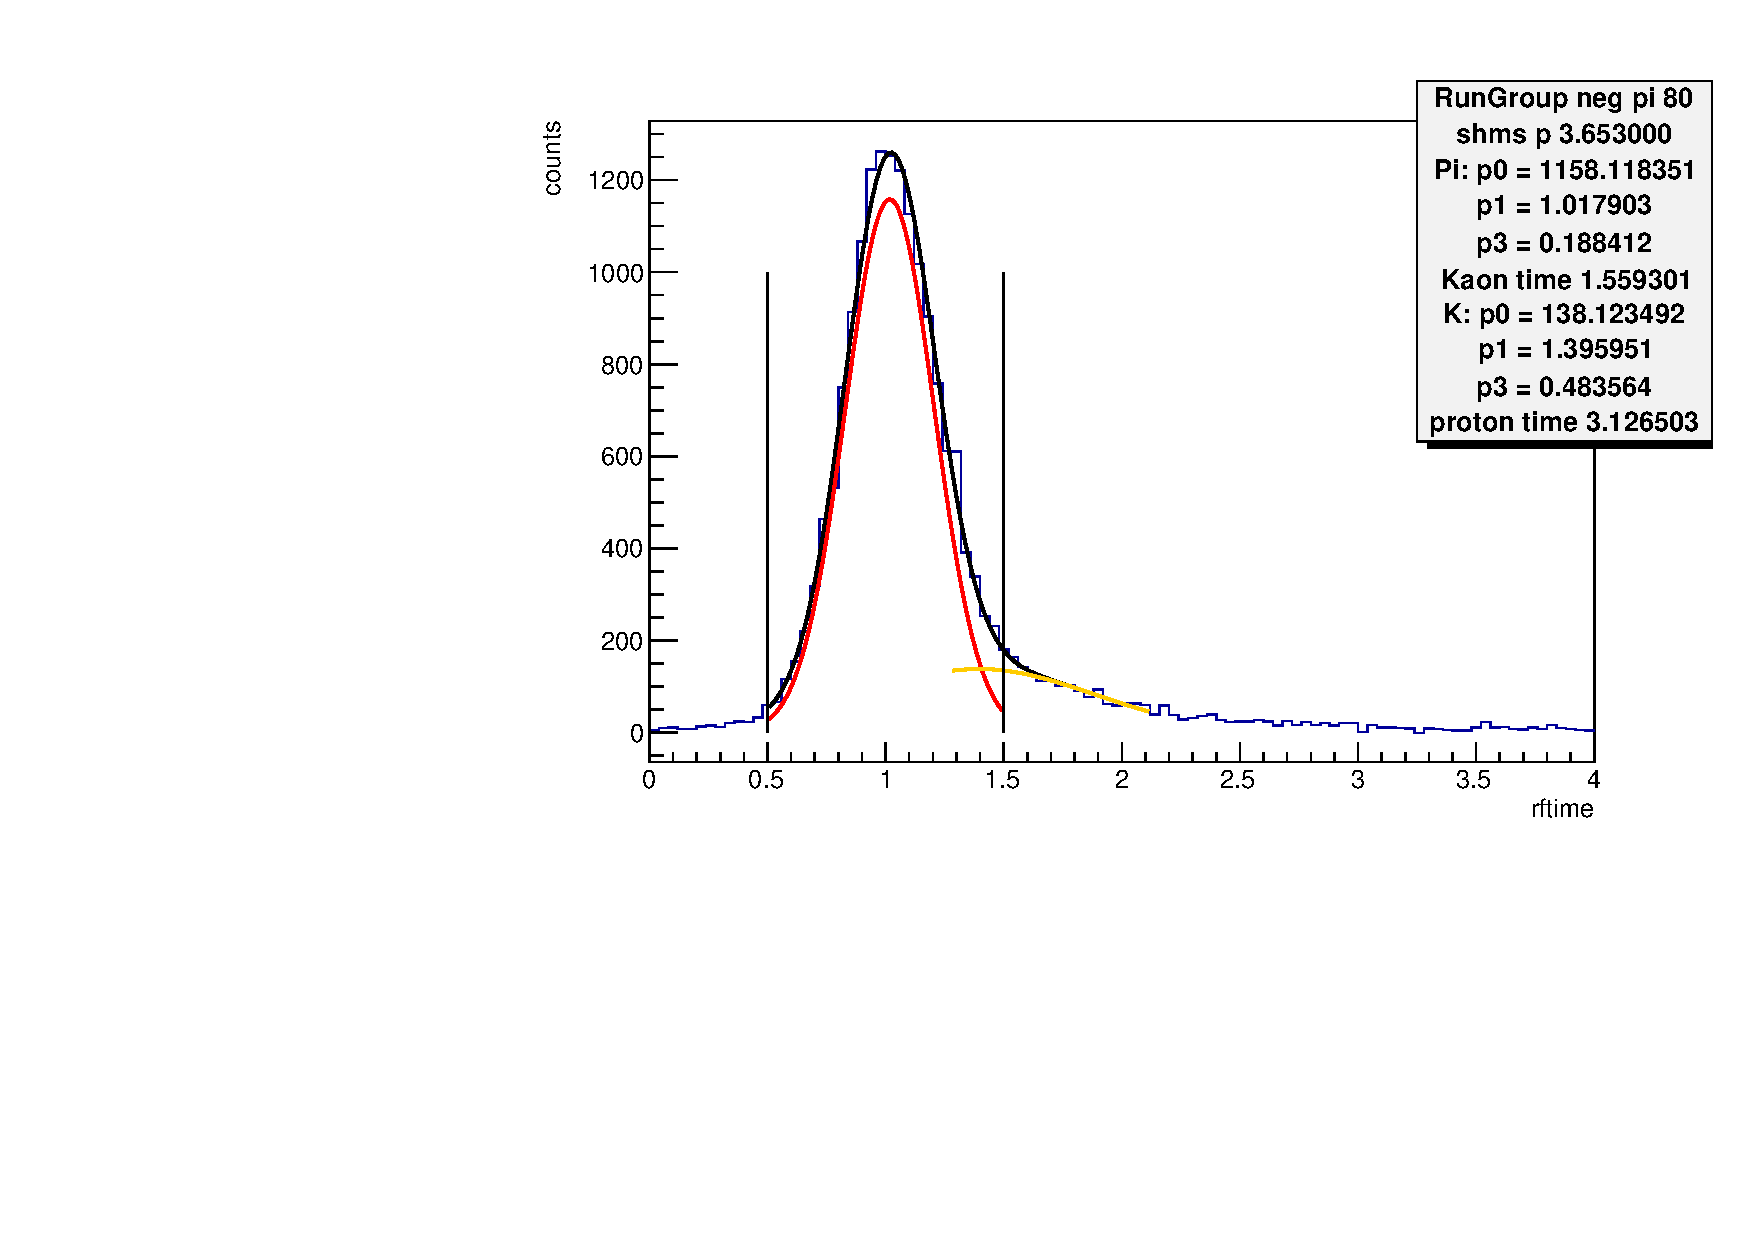
\includegraphics[width = 0.8\textwidth]{results/pid/rftime/rftime_neg_80_pi.pdf}
\end{column}
\begin{column}[T]{0.5\textwidth}
  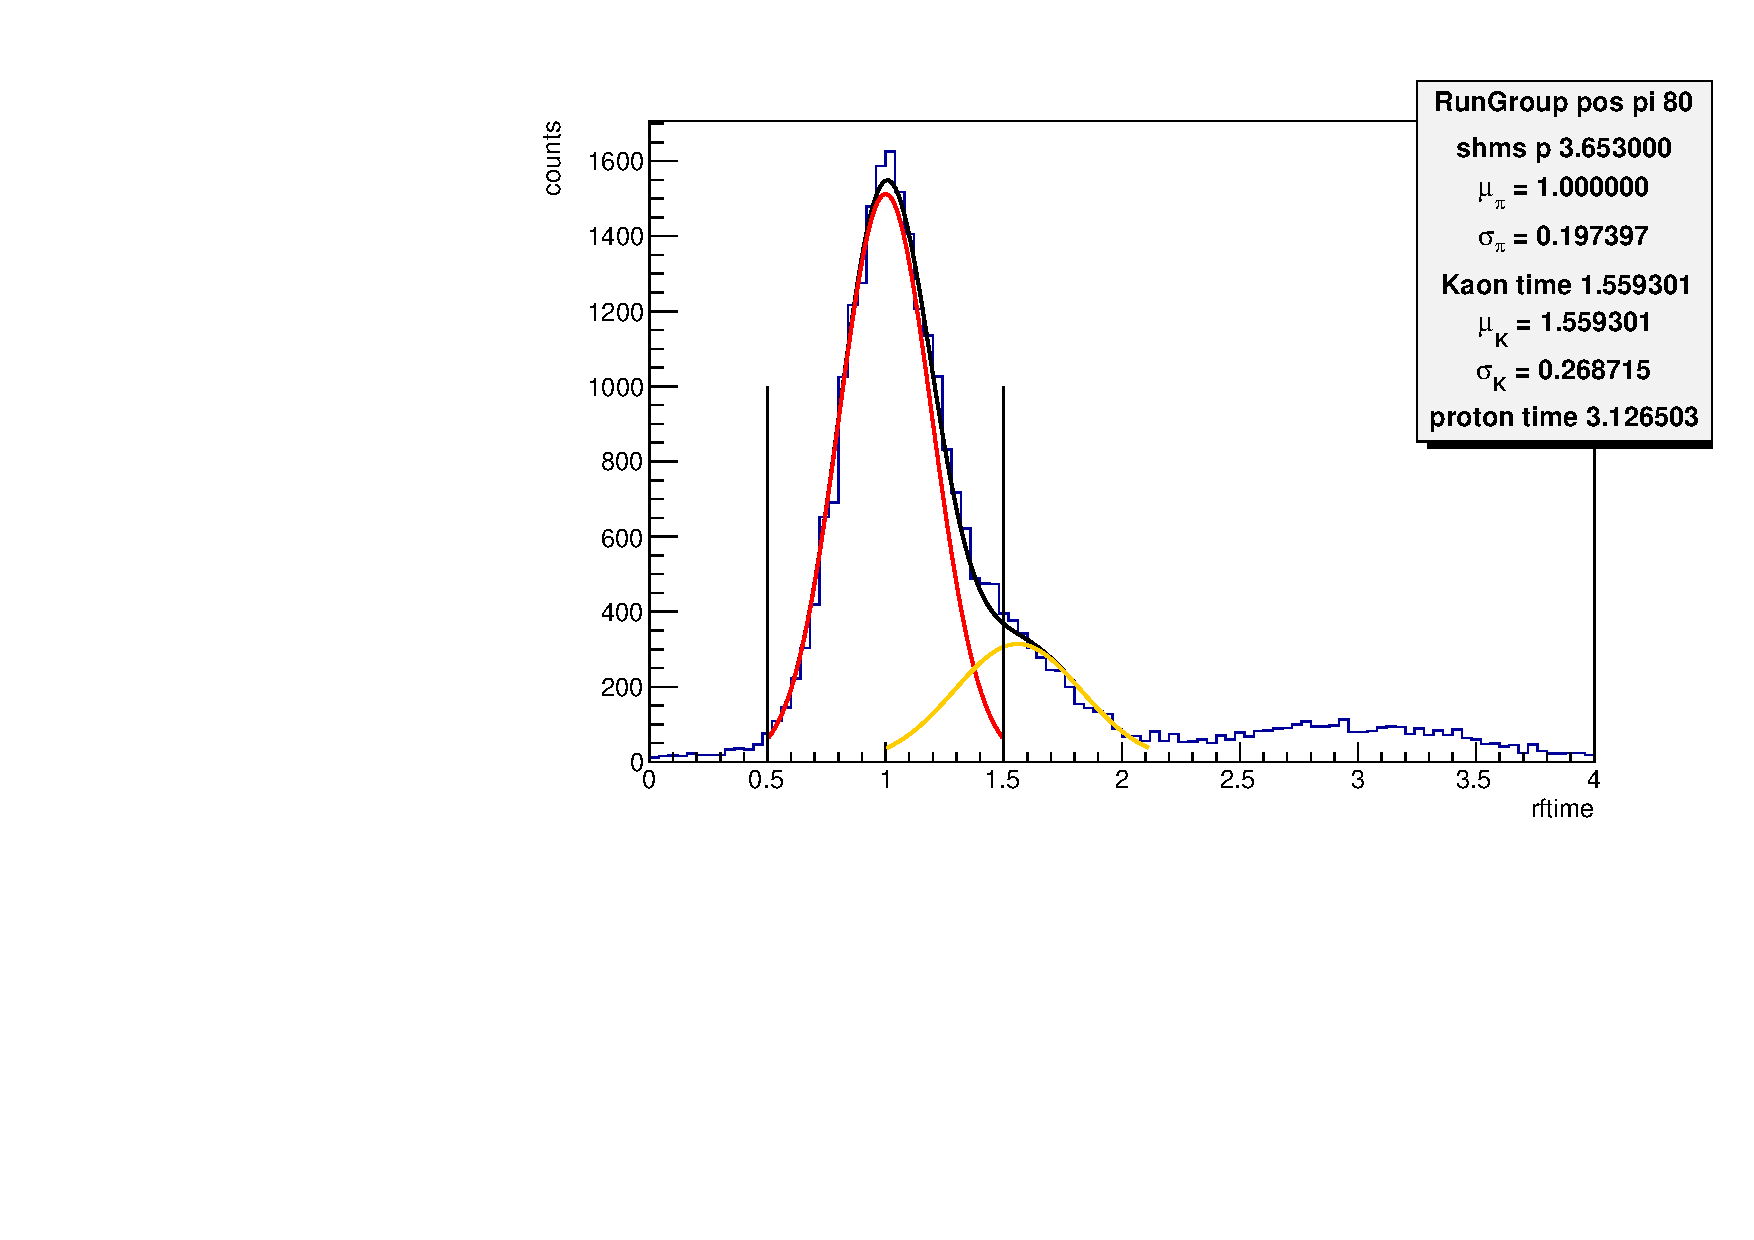
\includegraphics[width = 0.8\textwidth]{results/pid/rftime/rftime_pos_80_pi.pdf}
\end{column}
\end{columns}
\end{frame}

\begin{frame}  
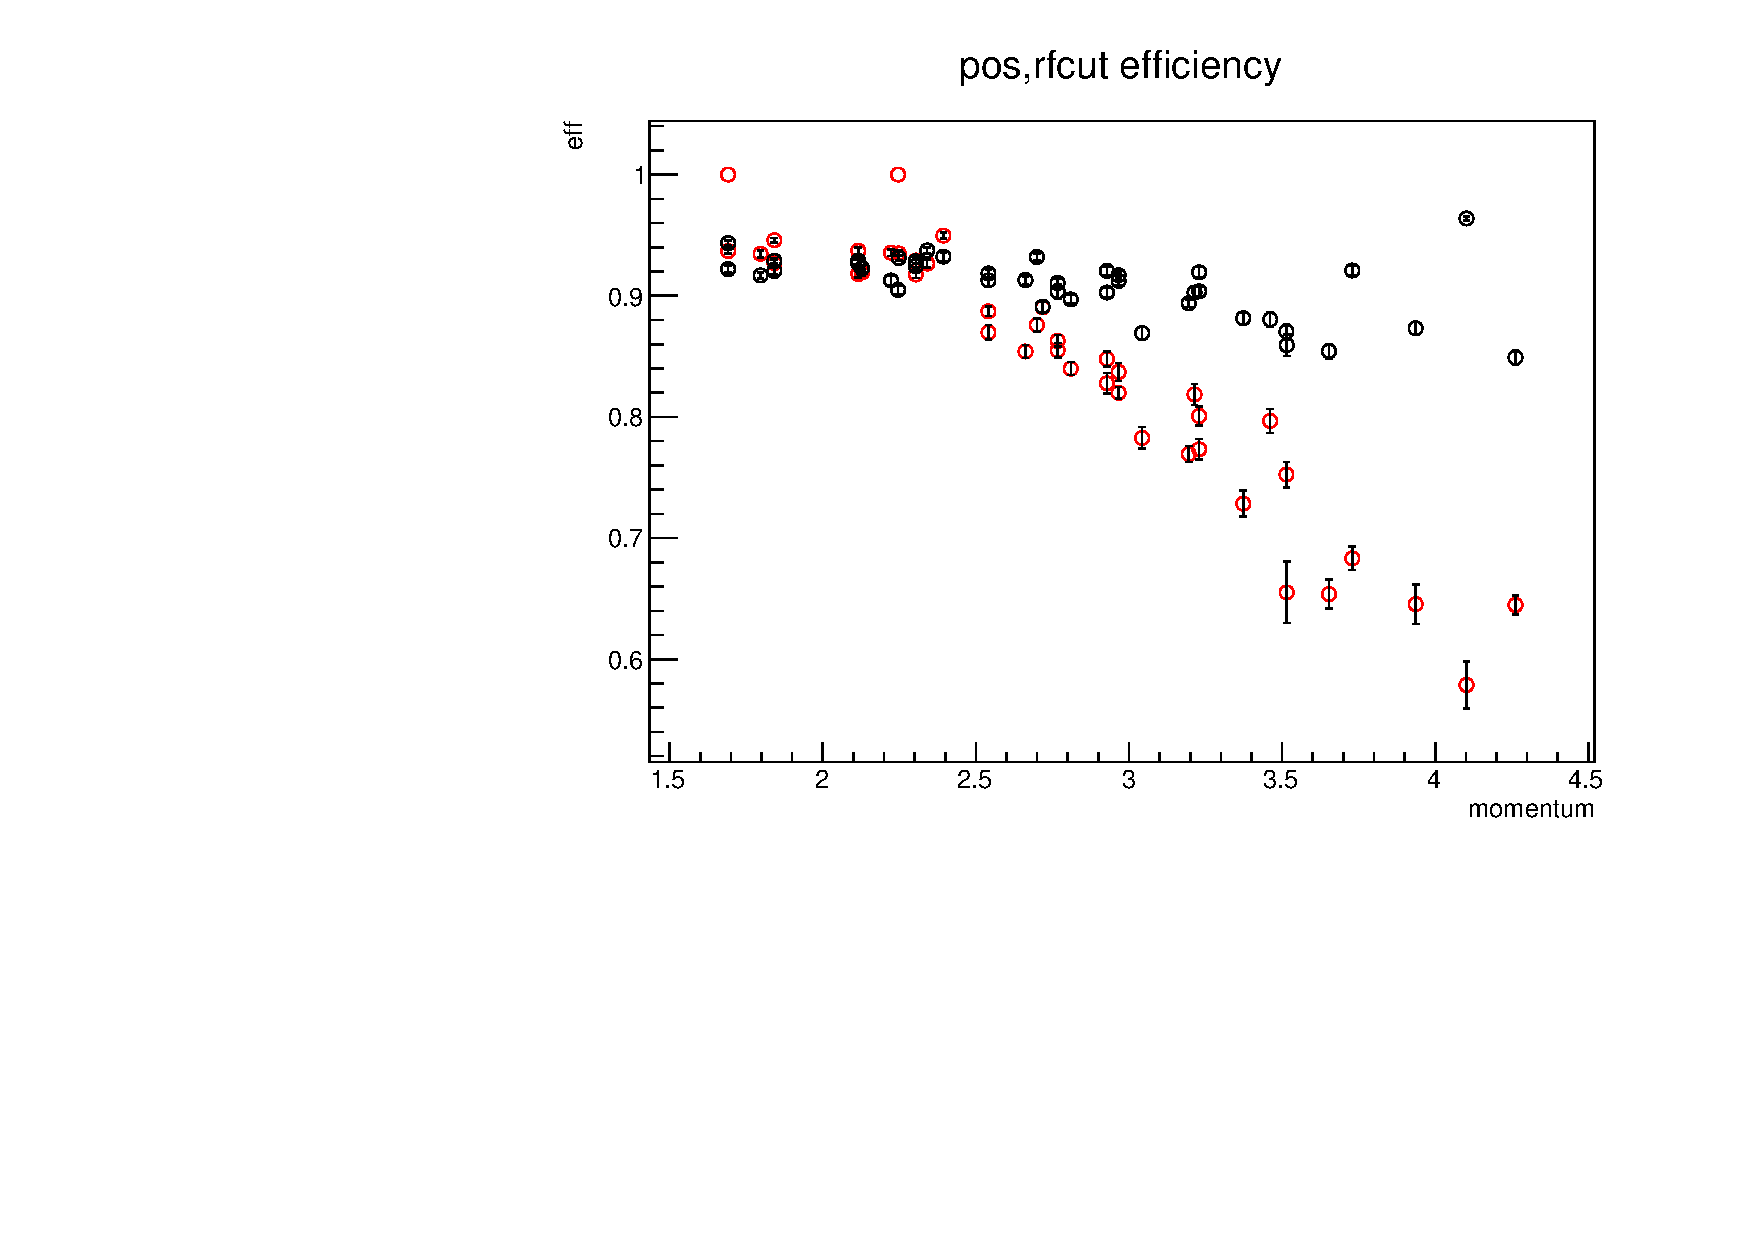
\includegraphics[width = 0.7\textwidth]{results/pid/SHMS_rf_momentum.pdf}
\\
pion eff from gaussian fit sigma estimate \\
kaon con = $\frac{kaonfit[new rfcut]}{allfit[new rfcut]}$
\\

\end{frame}
\begin{frame}{What if I use 3 sigma cut on pi fit}  
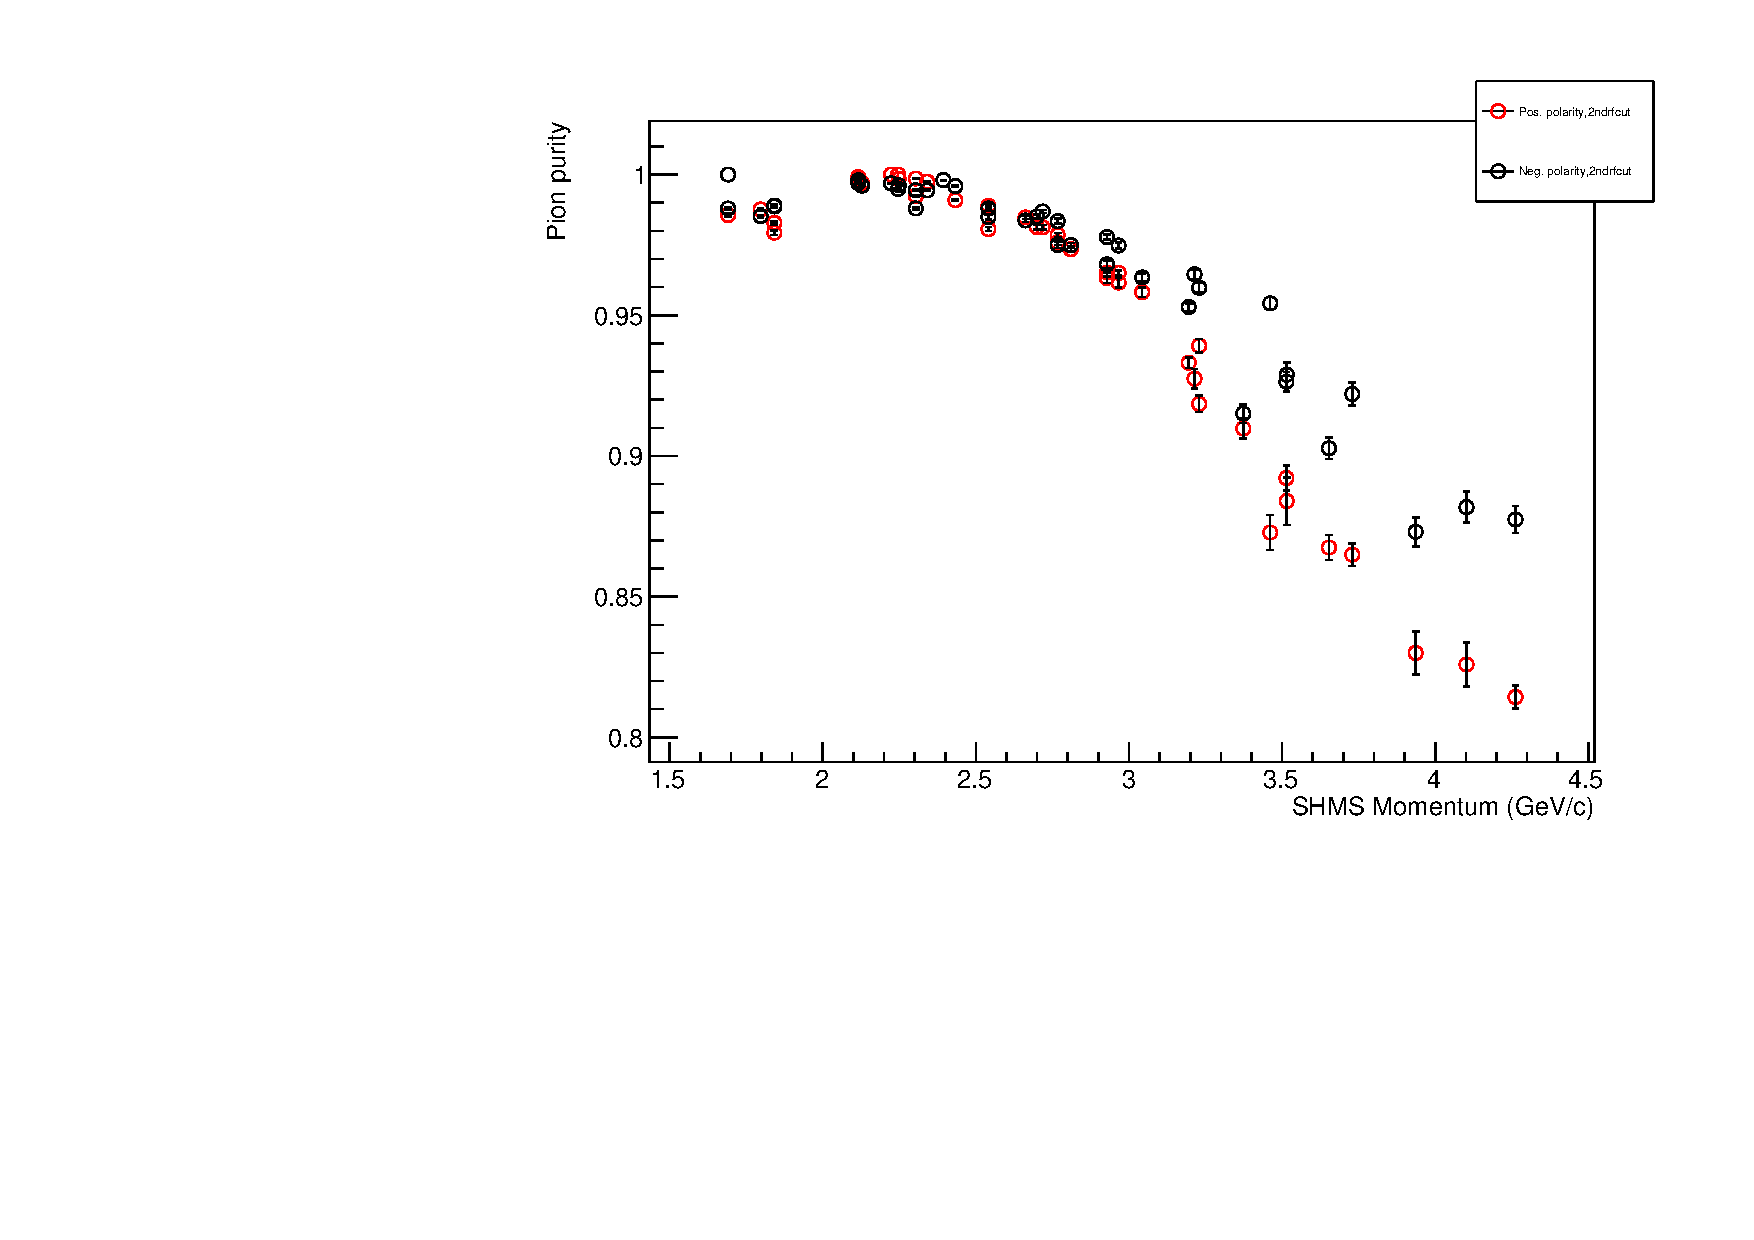
\includegraphics[width = 0.7\textwidth]{results/pid/SHMS_rf_momentum_2nd.pdf}
\\
pion eff = 99.7\\
kaon con = $\frac{kaonfit[new rfcut]}{allfit[new rfcut]}$
\end{frame}
\begin{frame}{150, SHMS momentum 3.936}
\begin{columns}
\begin{column}[T]{0.5\textwidth}
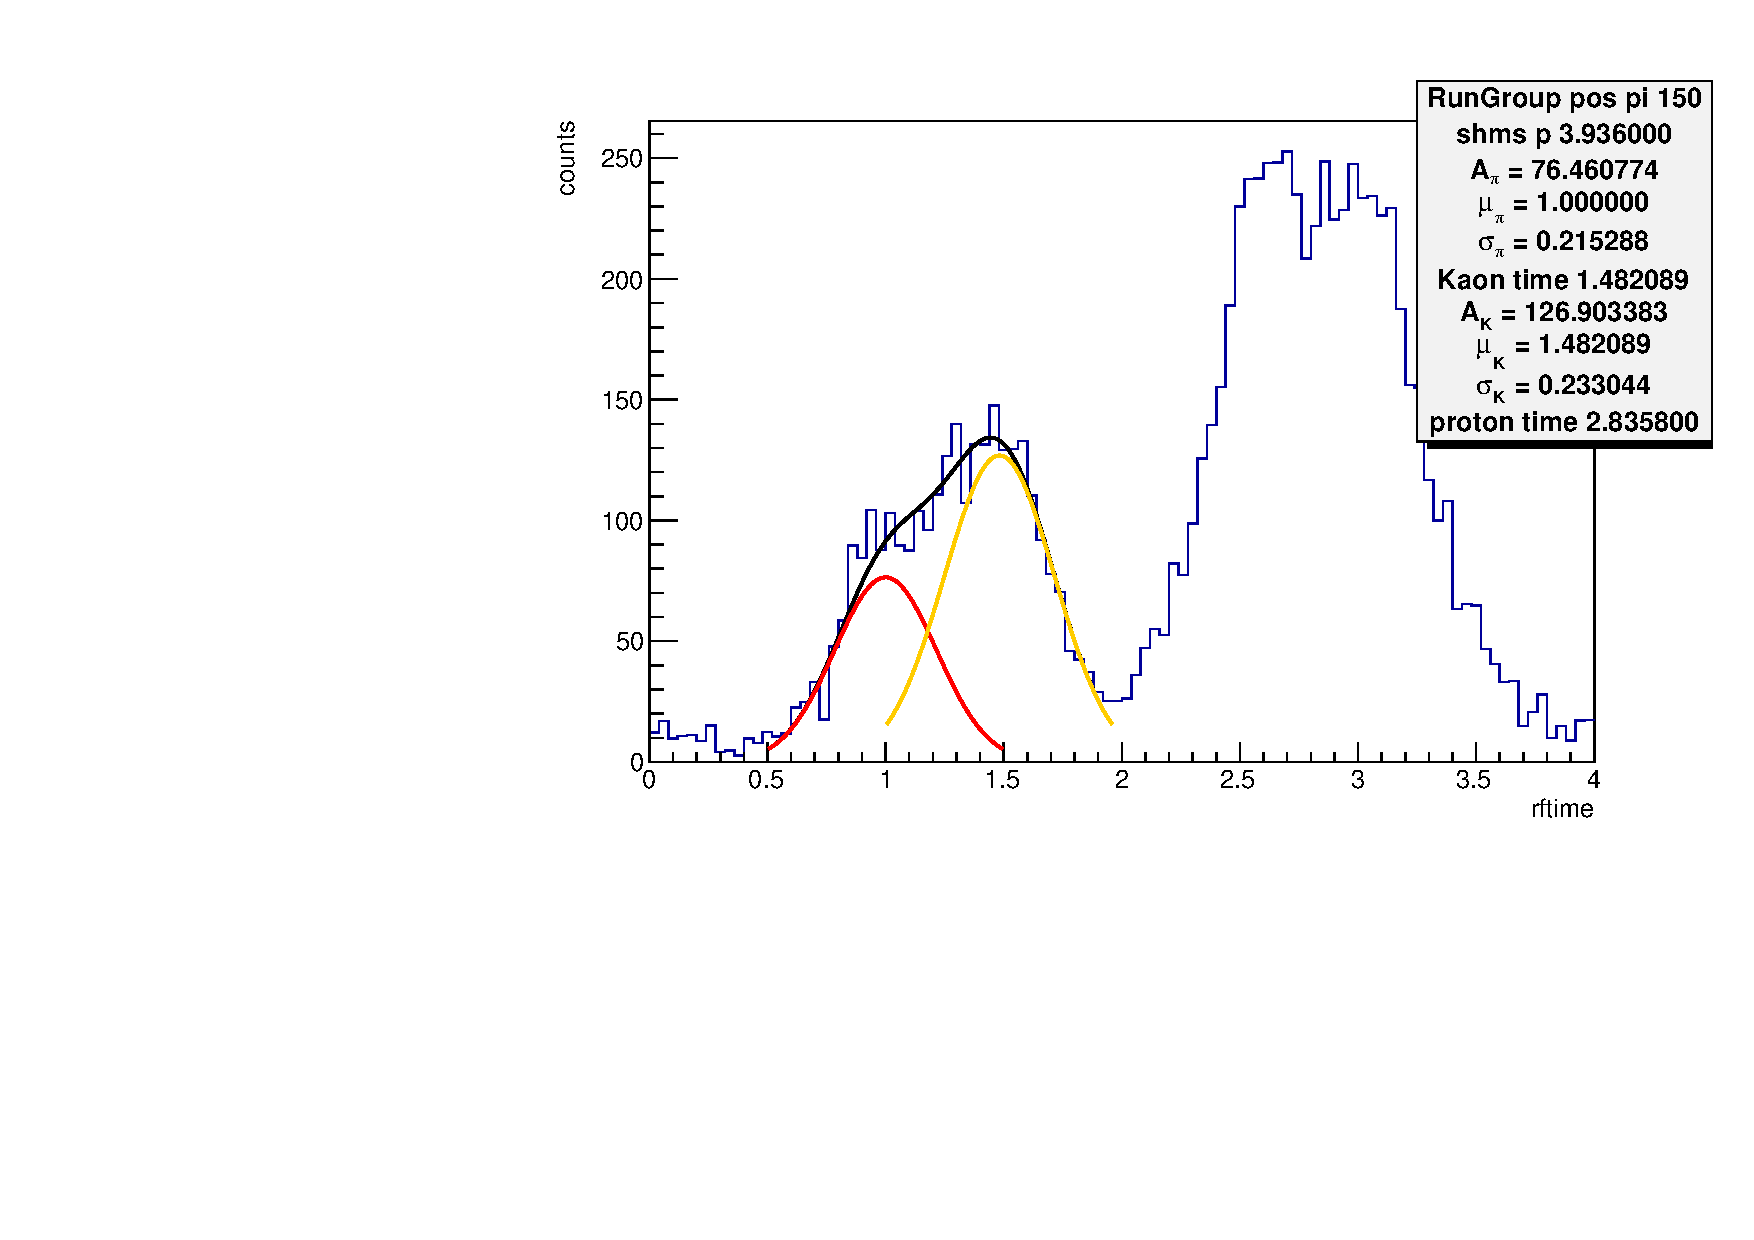
\includegraphics[width = 0.9\textwidth]{results/pid/rftime/rftime_pos_150.pdf}
\end{column}
\begin{column}[T]{0.5\textwidth}
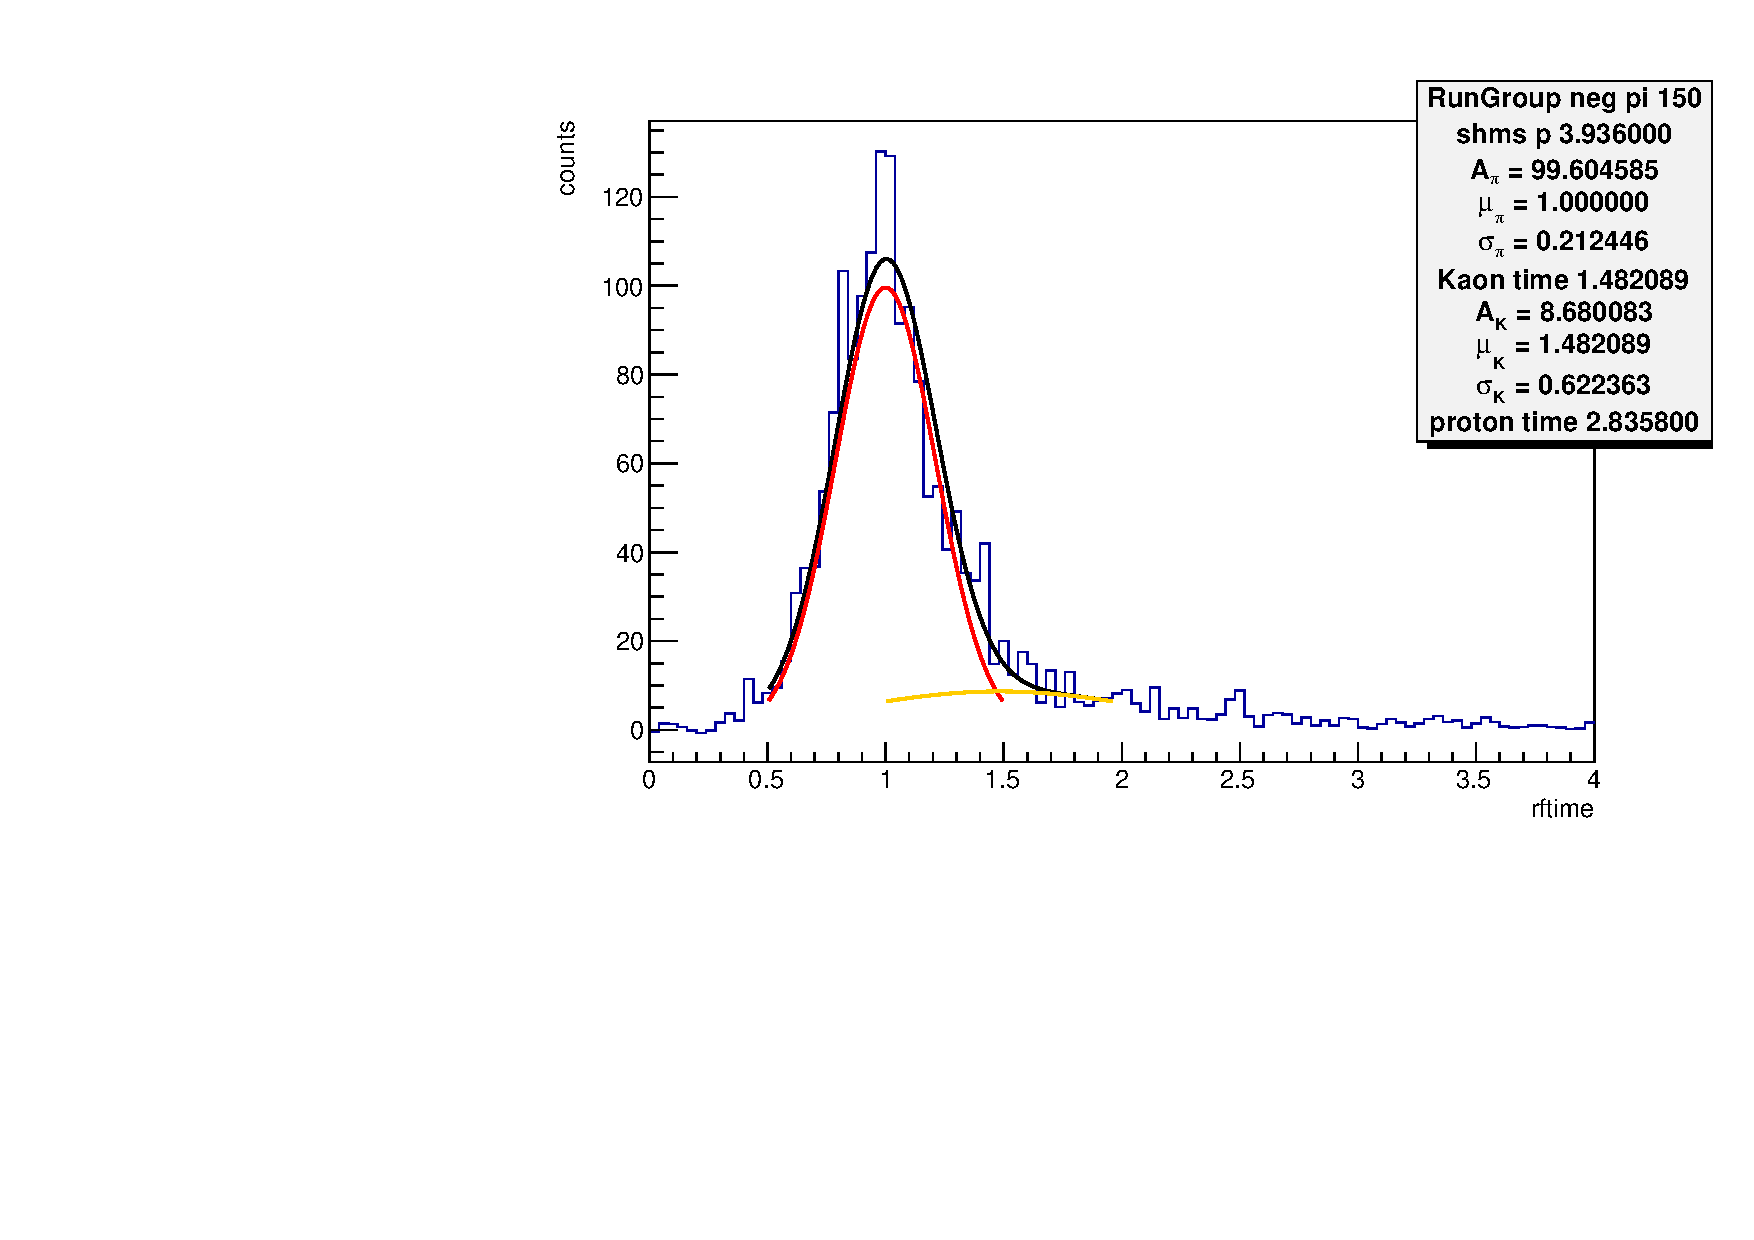
\includegraphics[width = 0.9\textwidth]{results/pid/rftime/rftime_neg_150.pdf}
\end{column}
\end{columns}
\end{frame}
\begin{frame}{150, SHMS momentum 3.936}
\begin{columns}
\begin{column}[T]{0.5\textwidth}
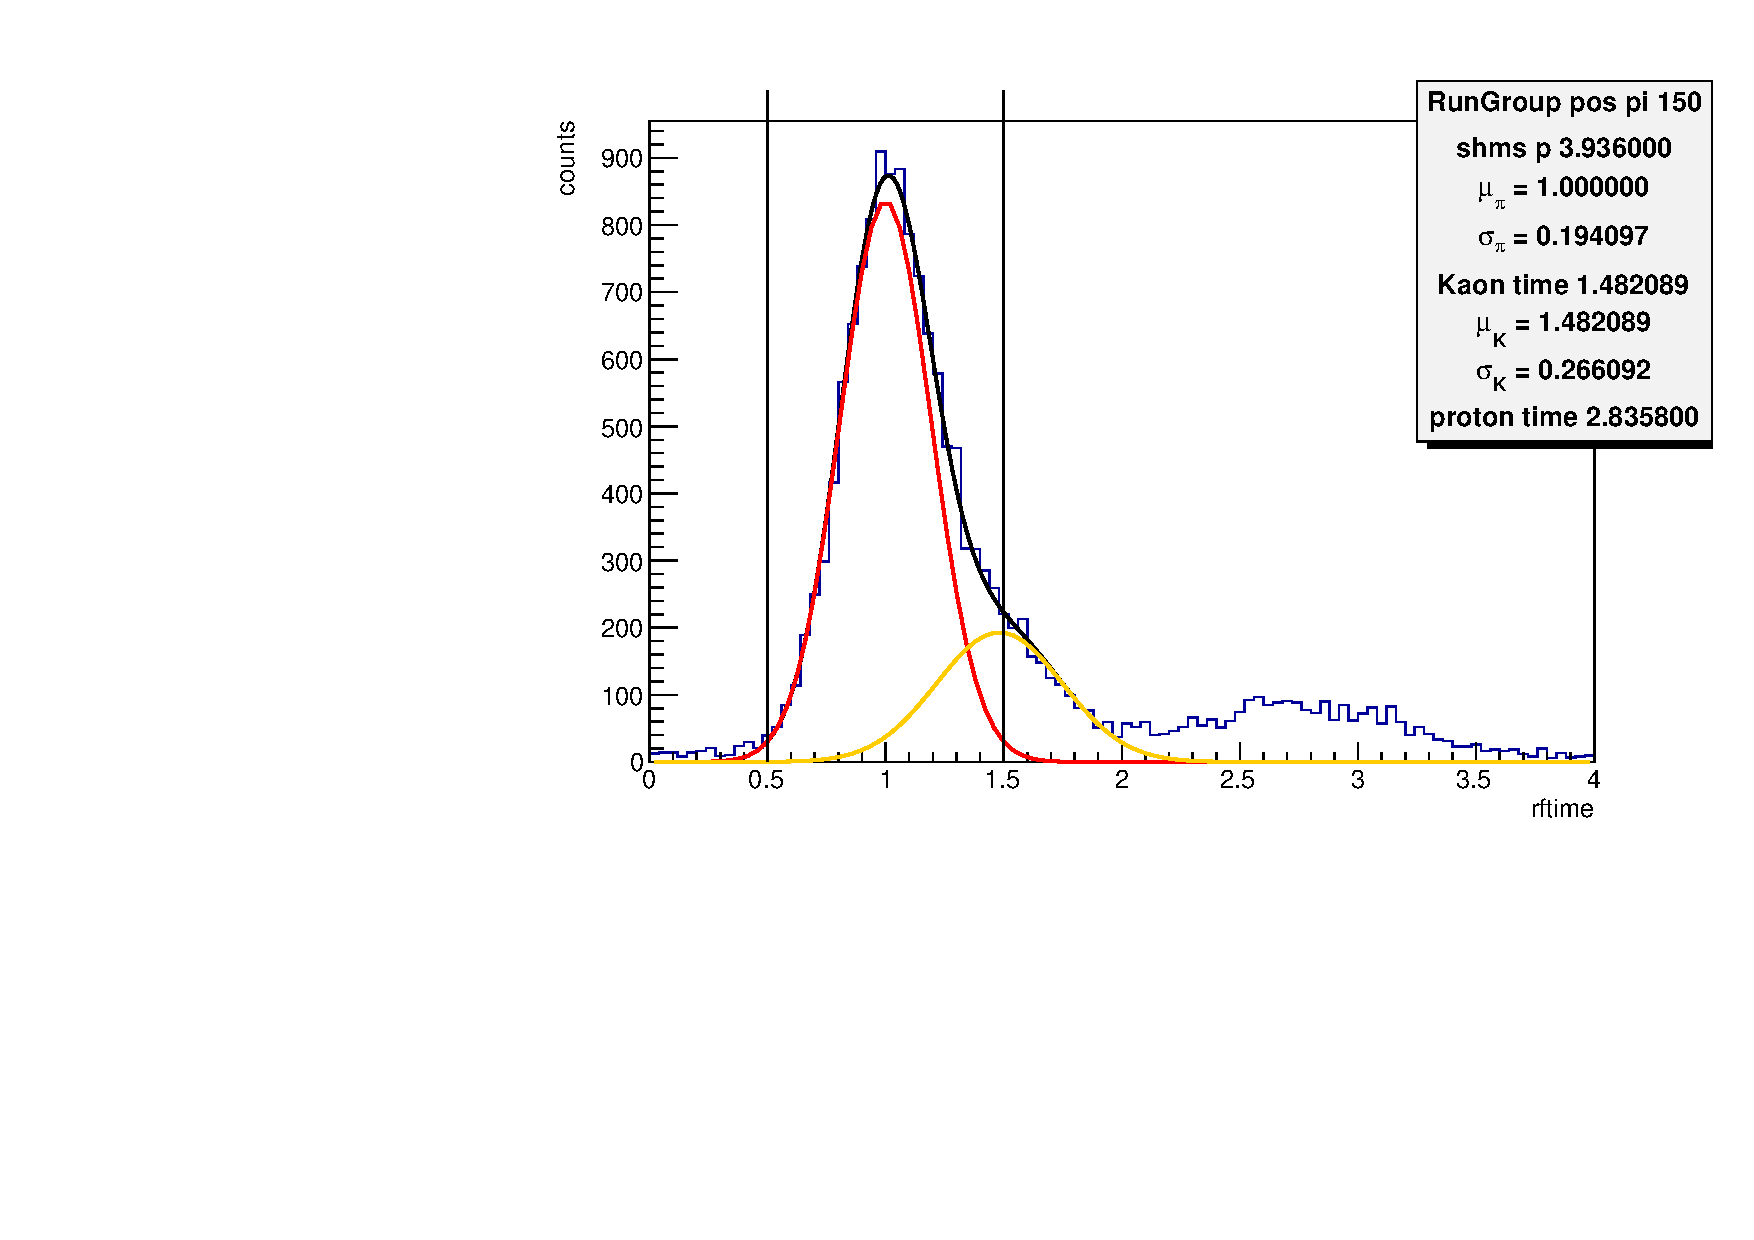
\includegraphics[width = 0.9\textwidth]{results/pid/rftime/rftime_pos_150_pi.pdf}
\end{column}
\begin{column}[T]{0.5\textwidth}
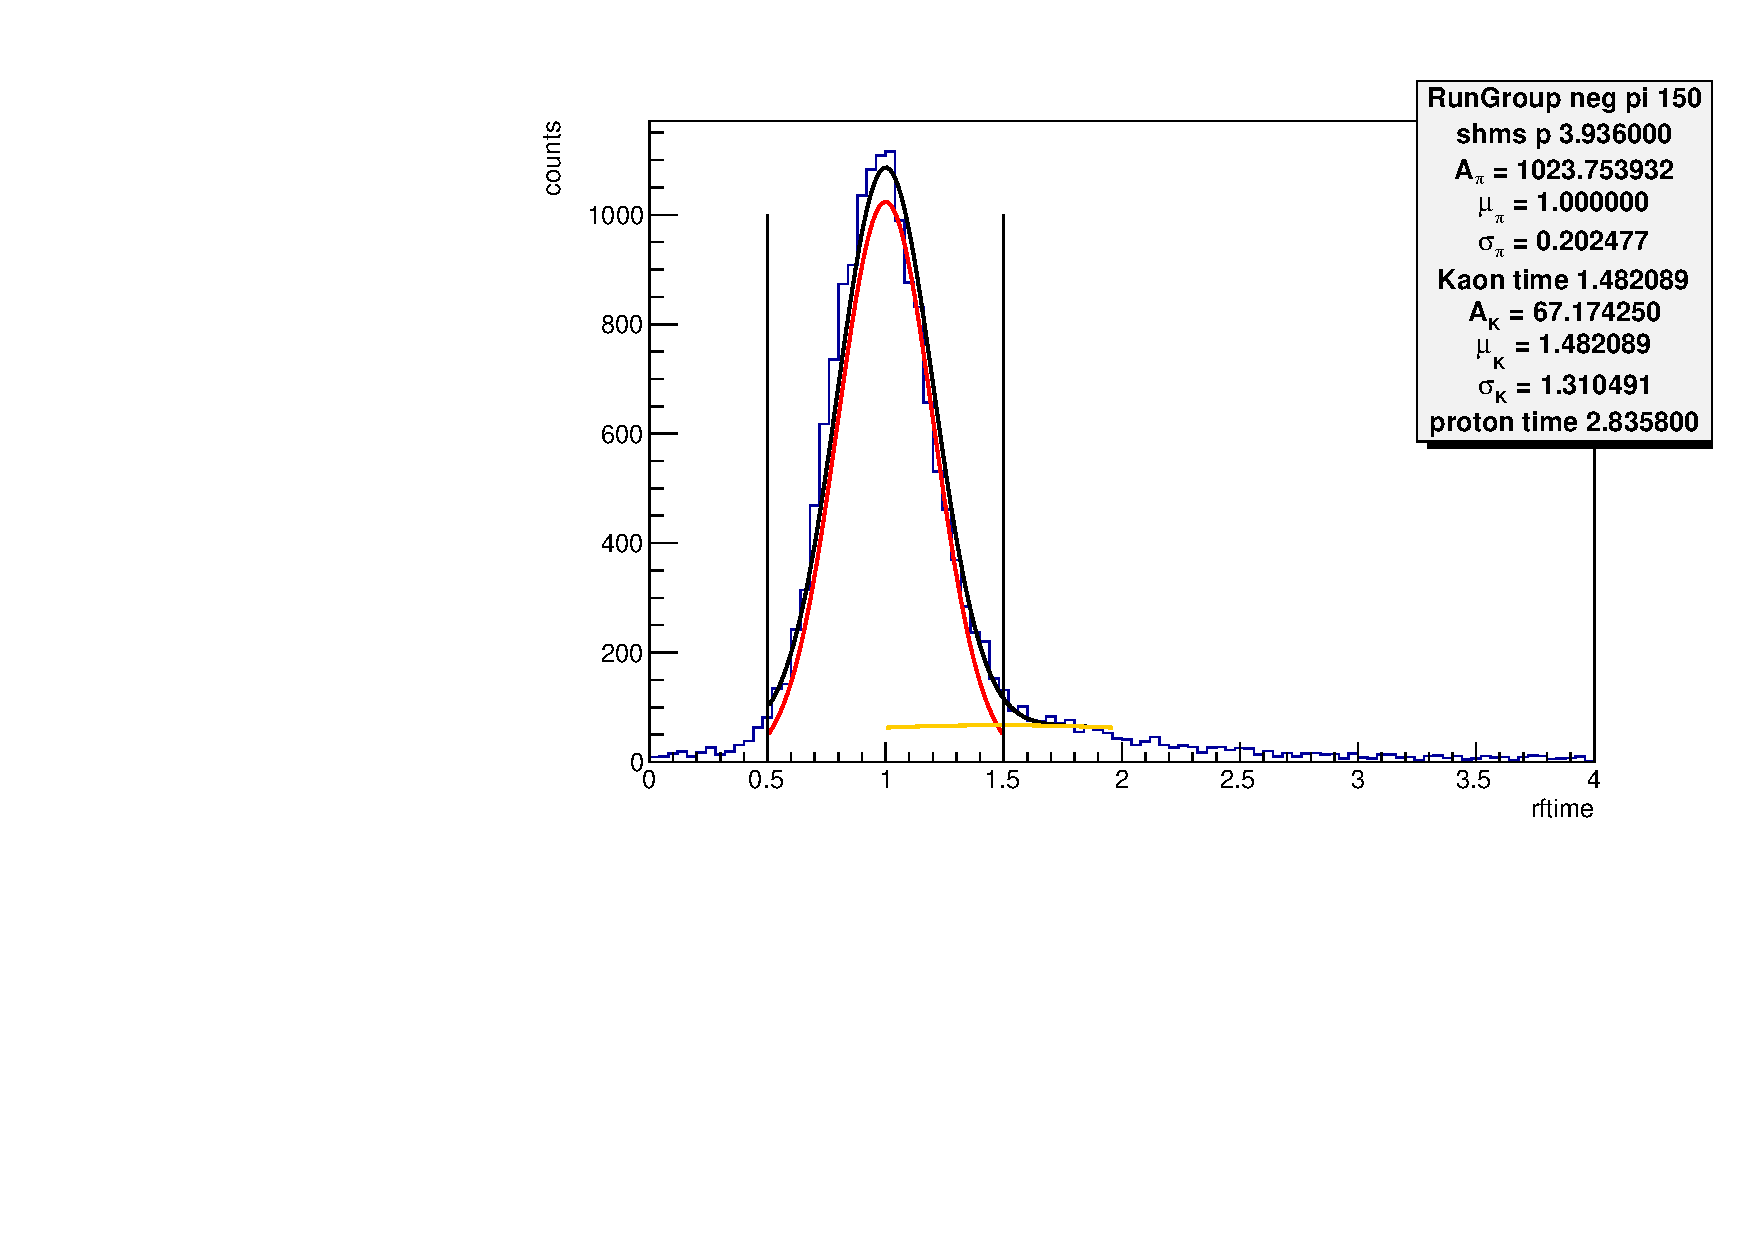
\includegraphics[width = 0.9\textwidth]{results/pid/rftime/rftime_neg_150_pi.pdf}
\end{column}
\end{columns}
\end{frame}
\begin{frame}{Some definition}
\begin{columns}
\begin{column}[T]{0.5\textwidth}
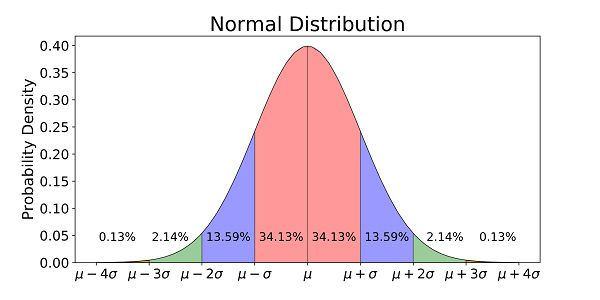
\includegraphics[width = \textwidth]{graphs/normal-distribution-curve.jpg}
\\pion efficiency = $\frac{pionfit[rfcut]}{pionfit[all range]}$
\end{column}
\begin{column}[T]{0.5\textwidth}
\includegraphics[width = 0.7\textwidth]{results/pid/rftime/rftime_pos_150_pi.pdf}
\\Kaon con. = $\frac{kaonfit[rfcut]}{pionfit[rfcut]}$
\end{column}
\end{columns}
\\
    \\For different rf timing cut,
    \\percentage: (Kpeak - Pipeak)*percentage + 1
  \\eg. pion peak at 1, kaon peak at 1.6, then percentage 80 means (1.6-1)*80\%+1 = 1.48, rf right hand side cut is at 1.48
\end{frame}

\begin{frame}{150, SHMS momentum 3.936}
\includegraphics[width = 0.7\textwidth]{results/pid/SHMS_rf_150_pos.pdf}
\\pion purity = 1-kaon con.
\end{frame}
\begin{frame}{150, SHMS momentum3.936}
\begin{columns}
\begin{column}[T]{0.5\textwidth}
HGC cut 0 \\
\includegraphics[width = 0.7\textwidth]{results/pid/SHMS_hgcer_eff_6194_0.pdf}
\end{column}
\begin{column}[T]{0.5\textwidth}
HGC cut 1 \\
\includegraphics[width = 0.7\textwidth]{results/pid/SHMS_hgcer_eff_6194_1.pdf}
\end{column}
\end{columns}
\begin{columns}
\begin{column}[T]{0.5\textwidth}
HGC cut 2 \\
\includegraphics[width = 0.7\textwidth]{results/pid/SHMS_hgcer_eff_6194_2.pdf}
\end{column}
\begin{column}[T]{0.5\textwidth}
HGC cut 3 \\
\includegraphics[width = 0.7\textwidth]{results/pid/SHMS_hgcer_eff_6194_3.pdf}
\end{column}
\end{columns}
\end{frame}
\begin{frame}{150, SHMS momentum 3.936}
\includegraphics[width = 0.7\textwidth]{results/pid/SHMS_hgcer_eff_6194_2_2d.pdf}
\end{frame}
%\begin{frame}{HGC eff uncertainty}
%    \begin{columns}
%    \begin{column}[T]{0.5\textwidth}
%    HGC cut 0 \\
%    \includegraphics[width = 0.7\textwidth]{results/pid/hgcer/x_Q2_0.35_4.00_0_xcer.pdf}
%    \end{column}
%     \begin{column}[T]{0.5\textwidth}
%     HGC cut 1 \\
%     \includegraphics[width = 0.7\textwidth]{results/pid/hgcer/x_Q2_0.35_4.00_1_xcer.pdf}
%    \end{column}
%    \end{columns}
%     \begin{columns}
%    \begin{column}[T]{0.5\textwidth}
%    HGC cut 2 \\
%    \includegraphics[width = 0.7\textwidth]{results/pid/hgcer/x_Q2_0.35_4.00_2_xcer.pdf}
%    \end{column}
%     \begin{column}[T]{0.5\textwidth}
%     HGC cut 3 \\
%     \includegraphics[width = 0.7\textwidth]{results/pid/hgcer/x_Q2_0.35_4.00_3_xcer.pdf}
%    \end{column}
%    \end{columns}
%\end{frame}
%\begin{frame}{HGC eff uncertainty}
%    \begin{columns}
%    \begin{column}[T]{0.5\textwidth}
%    HGC cut 0 \\
%    \includegraphics[width = 0.7\textwidth]{results/pid/hgcer/x_Q2_0.35_4.00_0_shmsp.pdf}
%    \end{column}
%     \begin{column}[T]{0.5\textwidth}
%     HGC cut 1 \\
%     \includegraphics[width = 0.7\textwidth]{results/pid/hgcer/x_Q2_0.35_4.00_1_shmsp.pdf}
%    \end{column}
%    \end{columns}
%     \begin{columns}
%    \begin{column}[T]{0.5\textwidth}
%    HGC cut 2 \\
%    \includegraphics[width = 0.7\textwidth]{results/pid/hgcer/x_Q2_0.35_4.00_2_shmsp.pdf}
%    \end{column}
%     \begin{column}[T]{0.5\textwidth}
%     HGC cut 3 \\
%     \includegraphics[width = 0.7\textwidth]{results/pid/hgcer/x_Q2_0.35_4.00_3_shmsp.pdf}
%    \end{column}
%    \end{columns}
%\end{frame}
%\begin{frame}{HGC cut 1, SHMS P }
%    \includegraphics[width = 0.8\textwidth]{results/pid/hgcer/x_Q2_0.35_4.00_1_shmsp.pdf}
%\end{frame}
%\begin{frame}{HGC cut 1, SHMS P }
%    \includegraphics[width = 0.8\textwidth]{results/pid/hgcer/x_Q2_0.35_4.00_1_xcer.pdf}
%\end{frame}
\begin{frame}{150, SHMS momentum 3.936}
HGC less than 2, no aero cut\\
\begin{columns}
\begin{column}[T]{0.33\textwidth}
first delta cut \\
\includegraphics[width = 0.9\textwidth]{results/pid/rftime/rftime_pos_150_0.pdf}
\end{column}
\begin{column}[T]{0.33\textwidth}
second delta cut \\
\includegraphics[width = 0.9\textwidth]{results/pid/rftime/rftime_pos_150_1.pdf}
\end{column}
\begin{column}[T]{0.33\textwidth}
delta cut \\
\includegraphics[width = 0.9\textwidth]{results/pid/rftime/rftime_pos_150_2.pdf}
\end{column}
\end{columns}
\begin{columns}
\begin{column}[T]{0.33\textwidth}
forth delta cut \\
\includegraphics[width = 0.9\textwidth]{results/pid/rftime/rftime_pos_150_3.pdf}
\end{column}
\begin{column}[T]{0.33\textwidth}
fifth delta cut \\
\includegraphics[width = 0.9\textwidth]{results/pid/rftime/rftime_pos_150_4.pdf}
\end{column}
\begin{column}[T]{0.33\textwidth}
sixth delta cut \\
\includegraphics[width = 0.9\textwidth]{results/pid/rftime/rftime_pos_150_5.pdf}
\end{column}
\end{columns}
\end{frame}
\begin{frame}{150,SHMS momentum 3.936}
\begin{columns}
\begin{column}[T]{0.3\textwidth}
first delta cut \\
\includegraphics[width = 0.9\textwidth]{results/pid/rftime/rftime_pos_150_0_pi.pdf}
\end{column}
\begin{column}[T]{0.3\textwidth}
second delta cut \\
\includegraphics[width = 0.9\textwidth]{results/pid/rftime/rftime_pos_150_1_pi.pdf}
\end{column}
\begin{column}[T]{0.3\textwidth}
third delta cut \\
\includegraphics[width = 0.9\textwidth]{results/pid/rftime/rftime_pos_150_2_pi.pdf}
\end{column}
\end{columns}
\begin{columns}
\begin{column}[T]{0.3\textwidth}
forth delta cut \\
\includegraphics[width = 0.9\textwidth]{results/pid/rftime/rftime_pos_150_3_pi.pdf}
\end{column}
\begin{column}[T]{0.3\textwidth}
fifth delta cut \\
\includegraphics[width = 0.9\textwidth]{results/pid/rftime/rftime_pos_150_4_pi.pdf}
\end{column}
\begin{column}[T]{0.3\textwidth}
sixth delta cut \\
\includegraphics[width = 0.9\textwidth]{results/pid/rftime/rftime_pos_150_5_pi.pdf}
\end{column}
\end{columns}
\end{frame}
\begin{frame}{150,SHMS momentum 3.936}
\begin{columns}
\begin{column}[T]{0.3\textwidth}
first delta cut \\
\includegraphics[width = 0.9\textwidth]{results/pid/SHMS_rf_150_0_pos.pdf}
\end{column}
\begin{column}[T]{0.3\textwidth}
second delta cut \\
\includegraphics[width = 0.9\textwidth]{results/pid/SHMS_rf_150_1_pos.pdf}
\end{column}
\begin{column}[T]{0.3\textwidth}
third delta cut \\
\includegraphics[width = 0.9\textwidth]{results/pid/SHMS_rf_150_2_pos.pdf}
\end{column}
\end{columns}
\begin{columns}
\begin{column}[T]{0.3\textwidth}
forth delta cut \\
\includegraphics[width = 0.9\textwidth]{results/pid/SHMS_rf_150_3_pos.pdf}
\end{column}
\begin{column}[T]{0.3\textwidth}
fifth delta cut \\
\includegraphics[width = 0.9\textwidth]{results/pid/SHMS_rf_150_4_pos.pdf}
\end{column}
\begin{column}[T]{0.3\textwidth}
sixth delta cut \\
\includegraphics[width = 0.9\textwidth]{results/pid/SHMS_rf_150_5_pos.pdf}
\end{column}
\end{columns}
\end{frame}

\begin{frame}
  backup
\end{frame}

\end{document}
 
